\documentclass{article}
\usepackage{amsmath}
\usepackage{color,pxfonts,fix-cm}
\usepackage{latexsym}
\usepackage[mathletters]{ucs}
\DeclareUnicodeCharacter{8220}{\textquotedblleft}
\DeclareUnicodeCharacter{46}{\textperiodcentered}
\DeclareUnicodeCharacter{8221}{\textquotedblright}
\DeclareUnicodeCharacter{58}{$\colon$}
\DeclareUnicodeCharacter{124}{\textbar}
\DeclareUnicodeCharacter{8226}{$\bullet$}
\DeclareUnicodeCharacter{8216}{\textquoteleft}
\DeclareUnicodeCharacter{62}{\textgreater}
\DeclareUnicodeCharacter{8593}{$\uparrow$}
\DeclareUnicodeCharacter{32}{$\ $}
\usepackage[T1]{fontenc}
\usepackage[utf8x]{inputenc}
\usepackage{pict2e}
\usepackage{wasysym}
\usepackage[english]{babel}
\usepackage{tikz}
\pagestyle{empty}
\usepackage[margin=0in,paperwidth=595pt,paperheight=841pt]{geometry}
\begin{document}
\definecolor{color_29791}{rgb}{0,0,0}
\definecolor{color_283006}{rgb}{1,1,1}
\definecolor{color_64546}{rgb}{0.137255,0.137255,0.137255}
\begin{tikzpicture}[overlay]\path(0pt,0pt);\end{tikzpicture}
\begin{picture}(-5,0)(2.5,0)
\put(95.06,-400.01){\fontsize{27.96}{1}\usefont{T1}{cmr}{b}{n}\selectfont\color{color_29791}Documentazione per Database }
\put(162.62,-442.27){\fontsize{27.96}{1}\usefont{T1}{cmr}{b}{n}\selectfont\color{color_29791}“Esame\_Traccia\_3” }
\put(282.65,-484.51){\fontsize{27.96}{1}\usefont{T1}{cmr}{b}{n}\selectfont\color{color_29791} }
\put(282.65,-526.63){\fontsize{27.96}{1}\usefont{T1}{cmr}{b}{n}\selectfont\color{color_29791} }
\put(218.93,-561.67){\fontsize{20.04}{1}\usefont{T1}{cmr}{m}{n}\selectfont\color{color_29791}Giuseppe Testa }
\put(232.85,-595.39){\fontsize{20.04}{1}\usefont{T1}{cmr}{m}{n}\selectfont\color{color_29791}N86004843 }
\put(282.65,-629.74){\fontsize{20.04}{1}\usefont{T1}{cmr}{m}{n}\selectfont\color{color_29791} }
\put(217.37,-662.38){\fontsize{20.04}{1}\usefont{T1}{cmr}{m}{n}\selectfont\color{color_29791}Andrea Pignieri }
\put(232.85,-696.1){\fontsize{20.04}{1}\usefont{T1}{cmr}{m}{n}\selectfont\color{color_29791}N86004636 }
\put(41.64,-735.456){\fontsize{27.96}{1}\usefont{T1}{cmr}{m}{n}\selectfont\color{color_29791} }
\put(58.425,-375.7301){
\includegraphics[width=448.45pt,height=315.8pt]{latexImage_7d51fbd63bd1a64c4a1f6cbb06aa82fd.png}}
\end{picture}
\newpage
\begin{tikzpicture}[overlay]\path(0pt,0pt);\end{tikzpicture}
\begin{picture}(-5,0)(2.5,0)
\put(41.64,-83.53998){\fontsize{27.96}{1}\usefont{T1}{cmr}{m}{n}\selectfont\color{color_29791}1 Progettazione concettuale }
\put(130.22,-117.14){\fontsize{27.96}{1}\usefont{T1}{cmr}{m}{n}\selectfont\color{color_29791} }
\put(41.64,-140.9){\fontsize{15.96}{1}\usefont{T1}{cmr}{b}{n}\selectfont\color{color_29791}1.1 Analisi e specifica dei requisiti }
\put(129.5,-160.46){\fontsize{15.96}{1}\usefont{T1}{cmr}{b}{n}\selectfont\color{color_29791} }
\put(41.64,-186.14){\fontsize{14.04}{1}\usefont{T1}{cmr}{m}{n}\selectfont\color{color_29791}Nella prima fase di analisi dei requisiti verranno identificate le informazioni }
\put(41.64,-202.94){\fontsize{14.04}{1}\usefont{T1}{cmr}{m}{n}\selectfont\color{color_29791}fondamentali che porteranno allo sviluppo della struttura e delle funzionalità del }
\put(41.64,-219.74){\fontsize{14.04}{1}\usefont{T1}{cmr}{m}{n}\selectfont\color{color_29791}database del cinema multisala. Durante il processo di analisi verranno individuate le }
\put(41.64,-236.54){\fontsize{14.04}{1}\usefont{T1}{cmr}{m}{n}\selectfont\color{color_29791}diverse entità, le relazioni che abbiamo tra di esse ed eventuali vincoli e }
\put(41.64,-253.34){\fontsize{14.04}{1}\usefont{T1}{cmr}{m}{n}\selectfont\color{color_29791}comportamenti del database. }
\put(41.64,-278.09){\fontsize{14.04}{1}\usefont{T1}{cmr}{m}{n}\selectfont\color{color_29791}Si sviluppi un sistema informativo per la gestione dei calciatori di tutti il mondo. Ogni }
\put(41.64,-294.89){\fontsize{14.04}{1}\usefont{T1}{cmr}{m}{n}\selectfont\color{color_29791}calciatore è caratterizzato da nome, cognome, data di nascita, piede (sinistro, destro o }
\put(41.64,-311.69){\fontsize{14.04}{1}\usefont{T1}{cmr}{m}{n}\selectfont\color{color_29791}ambidestro), uno o più ruoli di gioco (portiere, difensore, centrocampista, attaccante) }
\put(41.64,-328.49){\fontsize{14.04}{1}\usefont{T1}{cmr}{m}{n}\selectfont\color{color_29791}e una serie di feature caratteristiche (ad esempio colpo di testa, tackle, rovesciata, etc.). }
\put(41.64,-345.29){\fontsize{14.04}{1}\usefont{T1}{cmr}{m}{n}\selectfont\color{color_29791}Il giocatore ha una carriera durante la quale può militare in diverse squadre di calcio. }
\put(41.64,-362.09){\fontsize{14.04}{1}\usefont{T1}{cmr}{m}{n}\selectfont\color{color_29791}La militanza in una squadra è caratterizzata da uno o più periodi di tempo nei quali il }
\put(41.64,-378.89){\fontsize{14.04}{1}\usefont{T1}{cmr}{m}{n}\selectfont\color{color_29791}giocatore era in quella squadra. Ogni periodo di tempo ha una data inizio e data di }
\put(41.64,-395.69){\fontsize{14.04}{1}\usefont{T1}{cmr}{m}{n}\selectfont\color{color_29791}fine. Durante la militanza del giocatore nella squadra si tiene conto del numero di }
\put(41.64,-412.49){\fontsize{14.04}{1}\usefont{T1}{cmr}{m}{n}\selectfont\color{color_29791}partite giocate, del numero di goal segnati e del numero di goal subiti (applicabile solo }
\put(41.64,-429.29){\fontsize{14.04}{1}\usefont{T1}{cmr}{m}{n}\selectfont\color{color_29791}ai giocatori di ruolo portiere). Il giocatore può inoltre vincere trofei, individuali o di }
\put(41.64,-446.11){\fontsize{14.04}{1}\usefont{T1}{cmr}{m}{n}\selectfont\color{color_29791}squadra. Il giocatore può avere anche una data di ritiro a seguito della quale decide di }
\put(41.64,-462.91){\fontsize{14.04}{1}\usefont{T1}{cmr}{m}{n}\selectfont\color{color_29791}non giocare più. Le squadre di calcio sono specificate dal loro nome e nazionalità. }
\put(41.64,-479.71){\fontsize{14.04}{1}\usefont{T1}{cmr}{m}{n}\selectfont\color{color_29791}L’amministratore del sistema si identifica con una login ed una password e ha il diritto }
\put(41.64,-496.51){\fontsize{14.04}{1}\usefont{T1}{cmr}{m}{n}\selectfont\color{color_29791}di inserire nuovi giocatori nella base di dati, modificarne i dati, aggiungere ulteriori }
\put(41.64,-513.31){\fontsize{14.04}{1}\usefont{T1}{cmr}{m}{n}\selectfont\color{color_29791}informazioni oppure eliminare un giocatore. L’utente generico può vedere l’elenco dei }
\put(41.64,-530.11){\fontsize{14.04}{1}\usefont{T1}{cmr}{m}{n}\selectfont\color{color_29791}giocatori e le loro caratteristiche e può richiedere diverse ricerche, ad esempio }
\put(41.64,-546.91){\fontsize{14.04}{1}\usefont{T1}{cmr}{m}{n}\selectfont\color{color_29791}filtrando i giocatori per nome, per ruolo, per piede, per numero di goal segnati, per }
\put(41.64,-563.71){\fontsize{14.04}{1}\usefont{T1}{cmr}{m}{n}\selectfont\color{color_29791}numero di goal subiti, per età, per squadre di appartenenza. }
\put(41.64,-590.23){\fontsize{15.96}{1}\usefont{T1}{cmr}{m}{n}\selectfont\color{color_29791} }
\put(41.64,-617.38){\fontsize{15.96}{1}\usefont{T1}{cmr}{m}{n}\selectfont\color{color_29791} }
\put(41.64,-644.62){\fontsize{15.96}{1}\usefont{T1}{cmr}{m}{n}\selectfont\color{color_29791} }
\put(41.64,-671.86){\fontsize{15.96}{1}\usefont{T1}{cmr}{m}{n}\selectfont\color{color_29791} }
\put(41.64,-698.98){\fontsize{15.96}{1}\usefont{T1}{cmr}{m}{n}\selectfont\color{color_29791} }
\put(41.64,-726.22){\fontsize{15.96}{1}\usefont{T1}{cmr}{m}{n}\selectfont\color{color_29791} }
\put(41.64,-753.456){\fontsize{15.96}{1}\usefont{T1}{cmr}{m}{n}\selectfont\color{color_29791} }
\end{picture}
\newpage
\begin{tikzpicture}[overlay]\path(0pt,0pt);\end{tikzpicture}
\begin{picture}(-5,0)(2.5,0)
\put(41.64,-73.67999){\fontsize{15.96}{1}\usefont{T1}{cmr}{b}{n}\selectfont\color{color_29791}1.2 Diagramma concettuale }
\put(77.064,-99.38){\fontsize{14.04}{1}\usefont{T1}{cmr}{m}{n}\selectfont\color{color_29791} }
\put(41.64,-124.22){\fontsize{14.04}{1}\usefont{T1}{cmr}{m}{n}\selectfont\color{color_29791}Schema concettuale del database ottenuto dalle informazioni ricavate durante l’analisi }
\put(41.64,-141.02){\fontsize{14.04}{1}\usefont{T1}{cmr}{m}{n}\selectfont\color{color_29791}dei requisiti. }
\put(41.64,-164.3){\fontsize{11.04}{1}\usefont{T1}{cmr}{m}{n}\selectfont\color{color_29791} }
\put(41.64,-675.1){\fontsize{11.04}{1}\usefont{T1}{cmr}{m}{n}\selectfont\color{color_29791} }
\put(41.64,-699.1){\fontsize{14.04}{1}\usefont{T1}{cmr}{m}{n}\selectfont\color{color_29791} }
\put(41.64,-723.82){\fontsize{14.04}{1}\usefont{T1}{cmr}{m}{n}\selectfont\color{color_29791} }
\put(41.64,-748.656){\fontsize{14.04}{1}\usefont{T1}{cmr}{m}{n}\selectfont\color{color_29791} }
\put(10.4,-664.3){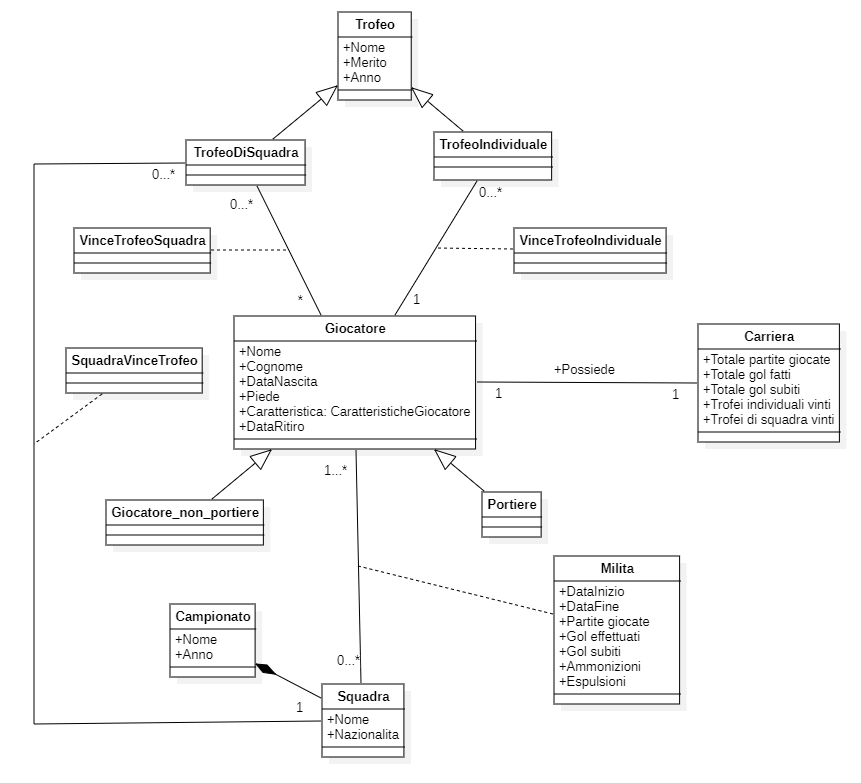
\includegraphics[width=543.79pt,height=494.7pt]{latexImage_5821dcf075b1270706fa51f8d6d51a90.png}}
\end{picture}
\newpage
\begin{tikzpicture}[overlay]\path(0pt,0pt);\end{tikzpicture}
\begin{picture}(-5,0)(2.5,0)
\put(41.64,-72.12){\fontsize{14.04}{1}\usefont{T1}{cmr}{m}{n}\selectfont\color{color_29791}Si consideri di voler partire dall’entità Giocatore, esso si specializza (totale, }
\put(41.64,-89.29999){\fontsize{14.04}{1}\usefont{T1}{cmr}{m}{n}\selectfont\color{color_29791}disgiunta) in Giocatore\_non\_portiere  e Portiere, ora iniziamo a descrivere la }
\put(41.64,-106.46){\fontsize{14.04}{1}\usefont{T1}{cmr}{m}{n}\selectfont\color{color_29791}relazione “Milita” che ha con l’entità Squadra; un giocatore può militare in nessuna }
\put(41.64,-123.14){\fontsize{14.04}{1}\usefont{T1}{cmr}{m}{n}\selectfont\color{color_29791}(qui la relazione è parziale in quanto un giocatore può anche ritirarsi) o più squadre }
\put(41.64,-139.94){\fontsize{14.04}{1}\usefont{T1}{cmr}{m}{n}\selectfont\color{color_29791}(in periodi di tempo differenti), e viceversa una squadra deve ospitare uno o più }
\put(41.64,-156.98){\fontsize{14.04}{1}\usefont{T1}{cmr}{m}{n}\selectfont\color{color_29791}giocatori. L’attributo GolSubiti verrà valorizzato solo se il giocatore è un portiere }
\put(41.64,-173.9){\fontsize{14.04}{1}\usefont{T1}{cmr}{m}{n}\selectfont\color{color_29791}(verrà risolto durante la fase successiva) }
\put(41.64,-198.62){\fontsize{14.04}{1}\usefont{T1}{cmr}{m}{n}\selectfont\color{color_29791}Successivamente un giocatore possiede una e una sola carriera, e viceversa una }
\put(41.64,-215.78){\fontsize{14.04}{1}\usefont{T1}{cmr}{m}{n}\selectfont\color{color_29791}carriera è posseduta da uno e un solo giocatore, si noti che l’entità Carriera serve per }
\put(41.64,-232.58){\fontsize{14.04}{1}\usefont{T1}{cmr}{m}{n}\selectfont\color{color_29791}avere un riassunto di tutte le statistiche del giocatore. }
\put(41.64,-257.81){\fontsize{14.04}{1}\usefont{T1}{cmr}{m}{n}\selectfont\color{color_29791}Un trofeo si specializza (totale, disgiunta) in Trofeo Individuale e Trofeo Di }
\put(41.64,-274.73){\fontsize{14.04}{1}\usefont{T1}{cmr}{b}{n}\selectfont\color{color_29791}Squadra. }
\put(41.64,-299.93){\fontsize{14.04}{1}\usefont{T1}{cmr}{m}{n}\selectfont\color{color_29791}Un giocatore può vincere nessuno o più trofei individuali, e viceversa un trofeo }
\put(41.64,-316.73){\fontsize{14.04}{1}\usefont{T1}{cmr}{m}{n}\selectfont\color{color_29791}individuale può essere vinto da uno e un solo giocatore.  }
\put(41.64,-341.93){\fontsize{14.04}{1}\usefont{T1}{cmr}{m}{n}\selectfont\color{color_29791}Un giocatore può vincere nessuno o più trofei di squadra, e viceversa un trofeo di }
\put(41.64,-358.61){\fontsize{14.04}{1}\usefont{T1}{cmr}{m}{n}\selectfont\color{color_29791}squadra può essere vinto da più giocatori.  }
\put(41.64,-383.81){\fontsize{14.04}{1}\usefont{T1}{cmr}{m}{n}\selectfont\color{color_29791}Analizzando l’entità Squadra passiamo ora a descrivere le sue relazioni, innanzitutto }
\put(41.64,-400.73){\fontsize{14.04}{1}\usefont{T1}{cmr}{m}{n}\selectfont\color{color_29791}le squadre andranno a comporre un Campionato, caratterizzato da un nome. }
\put(41.64,-425.69){\fontsize{14.04}{1}\usefont{T1}{cmr}{m}{n}\selectfont\color{color_29791}Infine una squadra può vincere uno o più trofei di squadra e viceversa un trofeo di }
\put(41.64,-442.51){\fontsize{14.04}{1}\usefont{T1}{cmr}{m}{n}\selectfont\color{color_29791}squadra può essere vinto da una e una sola squadra. }
\put(41.64,-467.23){\fontsize{14.04}{1}\usefont{T1}{cmr}{m}{n}\selectfont\color{color_29791} }
\put(41.64,-493.75){\fontsize{15.96}{1}\usefont{T1}{cmr}{m}{n}\selectfont\color{color_29791}  }
\end{picture}
\newpage
\begin{tikzpicture}[overlay]\path(0pt,0pt);\end{tikzpicture}
\begin{picture}(-5,0)(2.5,0)
\put(41.64,-84.14001){\fontsize{27.96}{1}\usefont{T1}{cmr}{b}{n}\selectfont\color{color_29791}2 Ristrutturazione }
\put(41.64,-114.02){\fontsize{14.04}{1}\usefont{T1}{cmr}{m}{n}\selectfont\color{color_29791} }
\put(41.64,-138.86){\fontsize{14.04}{1}\usefont{T1}{cmr}{m}{n}\selectfont\color{color_29791}Durante questa fase andremo a modificare alcuni aspetti del diagramma concettuale }
\put(41.64,-155.66){\fontsize{14.04}{1}\usefont{T1}{cmr}{m}{n}\selectfont\color{color_29791}al fine di renderlo più adatto per una traduzione al modello logico }
\put(41.64,-180.38){\fontsize{14.04}{1}\usefont{T1}{cmr}{m}{n}\selectfont\color{color_29791} }
\put(41.64,-207.14){\fontsize{15.96}{1}\usefont{T1}{cmr}{b}{n}\selectfont\color{color_29791}2.1 Analisi delle ridondanze }
\put(41.64,-232.82){\fontsize{14.04}{1}\usefont{T1}{cmr}{m}{n}\selectfont\color{color_29791}Abbiamo diverse ridondanze all’interno del diagramma concettuale, andiamo }
\put(41.64,-249.98){\fontsize{14.04}{1}\usefont{T1}{cmr}{m}{n}\selectfont\color{color_29791}innanzitutto ad intervenire sull’entità Carriera; essa ha attributi che sono delle }
\put(41.64,-266.69){\fontsize{14.04}{1}\usefont{T1}{cmr}{m}{n}\selectfont\color{color_29791}“estensioni” degli attributi delle relazioni “Milita”, quindi tutti i suoi dati sono già }
\put(41.64,-283.73){\fontsize{14.04}{1}\usefont{T1}{cmr}{m}{n}\selectfont\color{color_29791}reperibili, di conseguenza andremo ad eliminare l’entità Carriera. }
\put(41.64,-308.57){\fontsize{14.04}{1}\usefont{T1}{cmr}{m}{n}\selectfont\color{color_29791}Un’altra ridondanza che si può notare è la relazione “Vince\_trofeo\_squadra” in quanto }
\put(41.64,-325.37){\fontsize{14.04}{1}\usefont{T1}{cmr}{m}{n}\selectfont\color{color_29791}costituisce un’informazione reperibile già dalla relazione “SquadraVinceTrofeo” tra }
\put(41.64,-342.53){\fontsize{14.04}{1}\usefont{T1}{cmr}{m}{n}\selectfont\color{color_29791}l’entità Squadra e l’entità TrofeoDiSquadra; di conseguenza andremo ad eliminare }
\put(41.64,-359.33){\fontsize{14.04}{1}\usefont{T1}{cmr}{m}{n}\selectfont\color{color_29791}tale relazione. }
\put(41.64,-384.17){\fontsize{14.04}{1}\usefont{T1}{cmr}{m}{n}\selectfont\color{color_29791} }
\put(41.64,-410.81){\fontsize{15.96}{1}\usefont{T1}{cmr}{b}{n}\selectfont\color{color_29791}2.2 Analisi degli identificativi }
\put(41.64,-436.51){\fontsize{14.04}{1}\usefont{T1}{cmr}{m}{n}\selectfont\color{color_29791}In questa fase andremo a scegliere (o a creare) un attributo per identificare }
\put(41.64,-453.31){\fontsize{14.04}{1}\usefont{T1}{cmr}{m}{n}\selectfont\color{color_29791}univocamente le varie entità presenti nello schema precedente, in particolare: }
\put(76.944,-478.51){\fontsize{14.04}{1}\usefont{T1}{cmr}{m}{n}\selectfont\color{color_29791}1. L’entità Giocatore ha presente un insieme piuttosto ampio di chiavi }
\put(94.94,-495.19){\fontsize{14.04}{1}\usefont{T1}{cmr}{m}{n}\selectfont\color{color_29791}candidate, per questo motivo è stato scelto di aggiungere l’attributo }
\put(94.94,-512.23){\fontsize{14.04}{1}\usefont{T1}{cmr}{m}{it}\selectfont\color{color_29791}CodFiscale. }
\put(76.944,-529.39){\fontsize{14.04}{1}\usefont{T1}{cmr}{m}{n}\selectfont\color{color_29791}2. L’entità Squadra ha già presente l’attributo Nome che può fungere da }
\put(94.94,-546.31){\fontsize{14.04}{1}\usefont{T1}{cmr}{m}{n}\selectfont\color{color_29791}chiave primaria. }
\put(76.944,-563.35){\fontsize{14.04}{1}\usefont{T1}{cmr}{m}{n}\selectfont\color{color_29791}3. L’entità Campionato ha diverse chiavi candidate Nome, Anno, quindi per }
\put(94.94,-580.51){\fontsize{14.04}{1}\usefont{T1}{cmr}{m}{n}\selectfont\color{color_29791}semplificare gli accessi si è deciso di creare un attributo IdCampionato come }
\put(94.94,-597.31){\fontsize{14.04}{1}\usefont{T1}{cmr}{m}{n}\selectfont\color{color_29791}chiave primaria. }
\put(76.944,-614.38){\fontsize{14.04}{1}\usefont{T1}{cmr}{m}{n}\selectfont\color{color_29791}4. L’entità Trofeo ha due chiavi candidate (Nome, Anno), si è quindi deciso di }
\put(94.94,-631.3){\fontsize{14.04}{1}\usefont{T1}{cmr}{m}{n}\selectfont\color{color_29791}trasformarle entrambe in chiave primaria. }
\put(94.94,-648.1){\fontsize{14.04}{1}\usefont{T1}{cmr}{m}{n}\selectfont\color{color_29791} }
\put(94.94,-664.9){\fontsize{14.04}{1}\usefont{T1}{cmr}{m}{n}\selectfont\color{color_29791} }
\put(94.94,-681.7){\fontsize{14.04}{1}\usefont{T1}{cmr}{m}{n}\selectfont\color{color_29791} }
\put(41.64,-705.1){\fontsize{11.04}{1}\usefont{T1}{cmr}{m}{n}\selectfont\color{color_29791} }
\put(41.64,-727.54){\fontsize{11.04}{1}\usefont{T1}{cmr}{m}{n}\selectfont\color{color_29791} }
\put(41.64,-750.096){\fontsize{11.04}{1}\usefont{T1}{cmr}{m}{n}\selectfont\color{color_29791} }
\end{picture}
\newpage
\begin{tikzpicture}[overlay]\path(0pt,0pt);\end{tikzpicture}
\begin{picture}(-5,0)(2.5,0)
\put(41.64,-73.67999){\fontsize{15.96}{1}\usefont{T1}{cmr}{b}{n}\selectfont\color{color_29791} }
\put(41.64,-101.3){\fontsize{15.96}{1}\usefont{T1}{cmr}{b}{n}\selectfont\color{color_29791}2.3 Rimozione attributi multivalore }
\put(41.64,-126.98){\fontsize{14.04}{1}\usefont{T1}{cmr}{m}{n}\selectfont\color{color_29791}In questa fase andremo ad eliminare gli attributi che contengono delle liste di valori. }
\put(41.64,-151.7){\fontsize{14.04}{1}\usefont{T1}{cmr}{m}{n}\selectfont\color{color_29791}L’unico attributo multivalore presente nel diagramma concettuale è l’attributo }
\put(41.64,-168.74){\fontsize{14.04}{1}\usefont{T1}{cmr}{m}{it}\selectfont\color{color_29791}Caratteristica che indica una caratteristica particolare per quel giocatore, che per }
\put(41.64,-185.66){\fontsize{14.04}{1}\usefont{T1}{cmr}{m}{n}\selectfont\color{color_29791}l’appunto può essere anche più di una. }
\put(41.64,-210.74){\fontsize{14.04}{1}\usefont{T1}{cmr}{m}{n}\selectfont\color{color_29791}Andiamo ad aggiungere un’entità Caratteristica, con attributo Tipo\_caratteristica }
\put(41.64,-227.66){\fontsize{14.04}{1}\usefont{T1}{cmr}{m}{n}\selectfont\color{color_29791}che è anche chiave primaria. }
\put(41.64,-252.38){\fontsize{14.04}{1}\usefont{T1}{cmr}{m}{n}\selectfont\color{color_29791}Un giocatore può avere nessuna o più caratteristiche, viceversa una caratteristica }
\put(41.64,-269.21){\fontsize{14.04}{1}\usefont{T1}{cmr}{m}{n}\selectfont\color{color_29791}può essere posseduta da uno o più giocatori. }
\put(41.64,-294.05){\fontsize{14.04}{1}\usefont{T1}{cmr}{m}{n}\selectfont\color{color_29791} }
\put(41.64,-320.57){\fontsize{15.96}{1}\usefont{T1}{cmr}{m}{n}\selectfont\color{color_29791}                        }
\put(41.64,-347.93){\fontsize{15.96}{1}\usefont{T1}{cmr}{b}{n}\selectfont\color{color_29791}2.4 Rimozione attributi composti }
\put(41.64,-373.61){\fontsize{14.04}{1}\usefont{T1}{cmr}{m}{n}\selectfont\color{color_29791}Non sono presenti attributi composti. }
\put(41.64,-398.33){\fontsize{14.04}{1}\usefont{T1}{cmr}{m}{n}\selectfont\color{color_29791} }
\put(41.64,-425.09){\fontsize{14.04}{1}\usefont{T1}{cmr}{b}{n}\selectfont\color{color_29791}2.5 Partizione/Accorpamento delle associazioni }
\put(41.64,-450.79){\fontsize{14.04}{1}\usefont{T1}{cmr}{m}{n}\selectfont\color{color_29791}Non sono presenti associazioni 1:1. }
\put(41.64,-475.51){\fontsize{14.04}{1}\usefont{T1}{cmr}{m}{n}\selectfont\color{color_29791} }
\put(41.64,-502.27){\fontsize{15.96}{1}\usefont{T1}{cmr}{b}{n}\selectfont\color{color_29791}2.6 Rimozione delle gerarchie }
\put(41.64,-527.95){\fontsize{14.04}{1}\usefont{T1}{cmr}{m}{n}\selectfont\color{color_29791}In questo diagramma sono presenti 1 generalizzazione ed 1 composizione. In }
\put(41.64,-544.75){\fontsize{14.04}{1}\usefont{T1}{cmr}{m}{n}\selectfont\color{color_29791}particolare: }
\put(77.064,-569.83){\fontsize{14.04}{1}\usefont{T1}{cmr}{m}{n}\selectfont\color{color_29791}1. Per quanto riguarda la generalizzazione Trofeo, siccome è una totale }
\put(95.06,-586.63){\fontsize{14.04}{1}\usefont{T1}{cmr}{m}{n}\selectfont\color{color_29791}disgiunta, si è deciso di accorpare il padre nelle figlie, ottenendo come }
\put(95.06,-603.43){\fontsize{14.04}{1}\usefont{T1}{cmr}{m}{n}\selectfont\color{color_29791}risultato: }
\put(113.06,-622.54){\fontsize{14.04}{1}\usefont{T1}{cmr}{m}{n}\selectfont\color{color_29791}• Un’entità TrofeoIndividuale; e sarà in relazione con l’entità }
\put(131.06,-639.7){\fontsize{14.04}{1}\usefont{T1}{cmr}{b}{n}\selectfont\color{color_29791}Giocatore tramite la relazione “VinceTrofeoIndividuale” con }
\put(131.06,-656.38){\fontsize{14.04}{1}\usefont{T1}{cmr}{m}{n}\selectfont\color{color_29791}molteplicità 1:N }
\put(113.06,-675.46){\fontsize{14.04}{1}\usefont{T1}{cmr}{m}{n}\selectfont\color{color_29791}• Un’entità TrofeoDiSquadra; E sarà in relazione con l’entità }
\put(131.06,-692.62){\fontsize{14.04}{1}\usefont{T1}{cmr}{b}{n}\selectfont\color{color_29791}Squadra tramite la relazione “SquadraVinceTrofeo” con molteplicità }
\put(131.06,-709.42){\fontsize{14.04}{1}\usefont{T1}{cmr}{m}{n}\selectfont\color{color_29791}1:N. }
\put(77.064,-726.58){\fontsize{14.04}{1}\usefont{T1}{cmr}{m}{n}\selectfont\color{color_29791}2. Per quanto riguarda la generalizzazione Giocatore, siccome portiere non }
\put(95.06,-743.256){\fontsize{14.04}{1}\usefont{T1}{cmr}{m}{n}\selectfont\color{color_29791}ha attributi aggiuntivi e la generalizzazione è una totale disgiunta, si è }
\put(95.06,-760.056){\fontsize{14.04}{1}\usefont{T1}{cmr}{m}{n}\selectfont\color{color_29791}deciso di accorpare l’entità figlie nelle entità padre, ma se andassimo ad }
\end{picture}
\newpage
\begin{tikzpicture}[overlay]\path(0pt,0pt);\end{tikzpicture}
\begin{picture}(-5,0)(2.5,0)
\put(95.06,-72){\fontsize{14.04}{1}\usefont{T1}{cmr}{m}{n}\selectfont\color{color_29791}inserire all’interno dell’entità giocatore l’attributo Ruolo (per }
\put(95.06,-88.94){\fontsize{14.04}{1}\usefont{T1}{cmr}{m}{n}\selectfont\color{color_29791}l’identificazione del ruolo del giocatore), questo risulterà ridondante, in }
\put(95.06,-105.74){\fontsize{14.04}{1}\usefont{T1}{cmr}{m}{n}\selectfont\color{color_29791}quanto per rendere più dinamico il cambio di ruolo, da squadra in squadra, }
\put(95.06,-122.78){\fontsize{14.04}{1}\usefont{T1}{cmr}{m}{n}\selectfont\color{color_29791}si è deciso di inserire l’attributo Ruolo solo nell’associazione milita. }
\put(77.064,-140.06){\fontsize{14.04}{1}\usefont{T1}{cmr}{m}{n}\selectfont\color{color_29791}3. Infine per quanto riguarda la composizione di Campionato si è deciso di }
\put(95.06,-157.1){\fontsize{14.04}{1}\usefont{T1}{cmr}{m}{n}\selectfont\color{color_29791}creare una relazione tra essa e l’entità Squadra di molteplicità N:N, cioè: }
\put(119.66,-176.18){\fontsize{14.04}{1}\usefont{T1}{cmr}{m}{n}\selectfont\color{color_29791}• Una squadra compone uno o più campionati, viceversa un }
\put(137.66,-192.98){\fontsize{14.04}{1}\usefont{T1}{cmr}{m}{n}\selectfont\color{color_29791}campionato è composto da una o più squadre. }
\put(41.64,-217.7){\fontsize{14.04}{1}\usefont{T1}{cmr}{m}{n}\selectfont\color{color_29791} }
\put(41.64,-242.54){\fontsize{14.04}{1}\usefont{T1}{cmr}{m}{n}\selectfont\color{color_29791} }
\put(41.64,-269.33){\fontsize{15.96}{1}\usefont{T1}{cmr}{b}{n}\selectfont\color{color_29791}2.7 Diagramma UML ristrutturato }
\put(94.22,-288.89){\fontsize{15.96}{1}\usefont{T1}{cmr}{b}{n}\selectfont\color{color_29791} }
\put(94.22,-308.33){\fontsize{15.96}{1}\usefont{T1}{cmr}{b}{n}\selectfont\color{color_29791} }
\put(67.4,-773.58){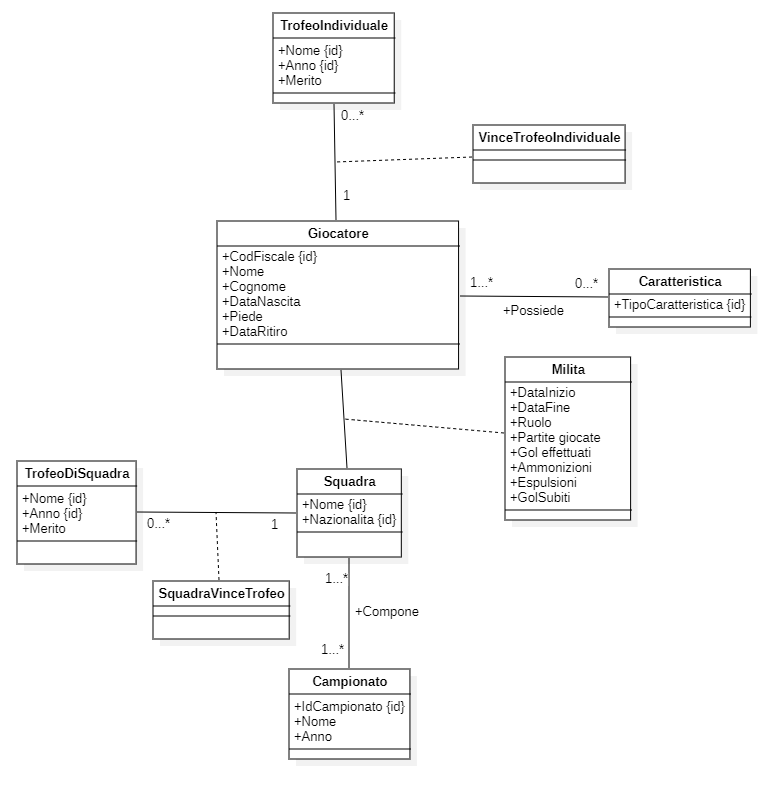
\includegraphics[width=429.82pt,height=443.3pt]{latexImage_16e133b8837f38b1b4a3bad46929b6ae.png}}
\end{picture}
\newpage
\begin{tikzpicture}[overlay]\path(0pt,0pt);\end{tikzpicture}
\begin{picture}(-5,0)(2.5,0)
\put(41.64,-71.76001){\fontsize{14.04}{1}\usefont{T1}{cmr}{m}{n}\selectfont\color{color_29791} }
\put(41.64,-103.82){\fontsize{21.96}{1}\usefont{T1}{cmr}{b}{n}\selectfont\color{color_29791}3 Dizionario delle classi, delle associazioni e }
\put(112.22,-130.7){\fontsize{21.96}{1}\usefont{T1}{cmr}{b}{n}\selectfont\color{color_29791}dei vincoli }
\put(112.22,-157.58){\fontsize{21.96}{1}\usefont{T1}{cmr}{b}{n}\selectfont\color{color_29791} }
\put(41.64,-179.18){\fontsize{15.96}{1}\usefont{T1}{cmr}{b}{n}\selectfont\color{color_29791}3.1 Dizionario delle classi }
\put(41.64,-206.78){\fontsize{15.96}{1}\usefont{T1}{cmr}{b}{n}\selectfont\color{color_29791} }
\put(47.88,-235.82){\fontsize{15.96}{1}\usefont{T1}{cmr}{b}{n}\selectfont\color{color_29791}Entità\;\;\;\;\;\;\;\;\;\;\;\;\;\;\;\;\;\;\;\;\;\;\;\; Descrizione\;\;\;\;\;\;\;\;\;\;\;\;\;\;\;\;\;\;\;\;\;\;\;\; Attributi }
\end{picture}
\begin{tikzpicture}[overlay]
\path(0pt,0pt);
\filldraw[color_29791][even odd rule]
(41.64pt, -222.02pt) -- (42.12pt, -222.02pt)
 -- (42.12pt, -222.02pt)
 -- (42.12pt, -220.46pt)
 -- (42.12pt, -220.46pt)
 -- (41.64pt, -220.46pt) -- cycle
;
\filldraw[color_29791][even odd rule]
(41.64pt, -220.94pt) -- (43.08pt, -220.94pt)
 -- (43.08pt, -220.94pt)
 -- (43.08pt, -220.46pt)
 -- (43.08pt, -220.46pt)
 -- (41.64pt, -220.46pt) -- cycle
;
\filldraw[color_29791][even odd rule]
(42.6pt, -222.02pt) -- (43.08pt, -222.02pt)
 -- (43.08pt, -222.02pt)
 -- (43.08pt, -221.42pt)
 -- (43.08pt, -221.42pt)
 -- (42.6pt, -221.42pt) -- cycle
;
\filldraw[color_29791][even odd rule]
(42.6pt, -221.9pt) -- (43.08pt, -221.9pt)
 -- (43.08pt, -221.9pt)
 -- (43.08pt, -221.42pt)
 -- (43.08pt, -221.42pt)
 -- (42.6pt, -221.42pt) -- cycle
;
\filldraw[color_29791][even odd rule]
(43.08pt, -220.94pt) -- (201.65pt, -220.94pt)
 -- (201.65pt, -220.94pt)
 -- (201.65pt, -220.46pt)
 -- (201.65pt, -220.46pt)
 -- (43.08pt, -220.46pt) -- cycle
;
\filldraw[color_29791][even odd rule]
(43.08pt, -221.9pt) -- (201.65pt, -221.9pt)
 -- (201.65pt, -221.9pt)
 -- (201.65pt, -221.42pt)
 -- (201.65pt, -221.42pt)
 -- (43.08pt, -221.42pt) -- cycle
;
\filldraw[color_29791][even odd rule]
(202.61pt, -222.02pt) -- (203.09pt, -222.02pt)
 -- (203.09pt, -222.02pt)
 -- (203.09pt, -221.9pt)
 -- (203.09pt, -221.9pt)
 -- (202.61pt, -221.9pt) -- cycle
;
\filldraw[color_29791][even odd rule]
(201.65pt, -222.02pt) -- (202.13pt, -222.02pt)
 -- (202.13pt, -222.02pt)
 -- (202.13pt, -221.9pt)
 -- (202.13pt, -221.9pt)
 -- (201.65pt, -221.9pt) -- cycle
;
\filldraw[color_29791][even odd rule]
(201.65pt, -220.94pt) -- (203.09pt, -220.94pt)
 -- (203.09pt, -220.94pt)
 -- (203.09pt, -220.46pt)
 -- (203.09pt, -220.46pt)
 -- (201.65pt, -220.46pt) -- cycle
;
\filldraw[color_29791][even odd rule]
(201.65pt, -221.9pt) -- (202.13pt, -221.9pt)
 -- (202.13pt, -221.9pt)
 -- (202.13pt, -221.42pt)
 -- (202.13pt, -221.42pt)
 -- (201.65pt, -221.42pt) -- cycle
;
\filldraw[color_29791][even odd rule]
(202.61pt, -221.9pt) -- (203.09pt, -221.9pt)
 -- (203.09pt, -221.9pt)
 -- (203.09pt, -221.42pt)
 -- (203.09pt, -221.42pt)
 -- (202.61pt, -221.42pt) -- cycle
;
\filldraw[color_29791][even odd rule]
(203.09pt, -220.94pt) -- (361.75pt, -220.94pt)
 -- (361.75pt, -220.94pt)
 -- (361.75pt, -220.46pt)
 -- (361.75pt, -220.46pt)
 -- (203.09pt, -220.46pt) -- cycle
;
\filldraw[color_29791][even odd rule]
(203.09pt, -221.9pt) -- (361.75pt, -221.9pt)
 -- (361.75pt, -221.9pt)
 -- (361.75pt, -221.42pt)
 -- (361.75pt, -221.42pt)
 -- (203.09pt, -221.42pt) -- cycle
;
\filldraw[color_29791][even odd rule]
(362.71pt, -222.02pt) -- (363.19pt, -222.02pt)
 -- (363.19pt, -222.02pt)
 -- (363.19pt, -221.9pt)
 -- (363.19pt, -221.9pt)
 -- (362.71pt, -221.9pt) -- cycle
;
\filldraw[color_29791][even odd rule]
(361.75pt, -222.02pt) -- (362.23pt, -222.02pt)
 -- (362.23pt, -222.02pt)
 -- (362.23pt, -221.9pt)
 -- (362.23pt, -221.9pt)
 -- (361.75pt, -221.9pt) -- cycle
;
\filldraw[color_29791][even odd rule]
(361.75pt, -220.94pt) -- (363.19pt, -220.94pt)
 -- (363.19pt, -220.94pt)
 -- (363.19pt, -220.46pt)
 -- (363.19pt, -220.46pt)
 -- (361.75pt, -220.46pt) -- cycle
;
\filldraw[color_29791][even odd rule]
(361.75pt, -221.9pt) -- (362.23pt, -221.9pt)
 -- (362.23pt, -221.9pt)
 -- (362.23pt, -221.42pt)
 -- (362.23pt, -221.42pt)
 -- (361.75pt, -221.42pt) -- cycle
;
\filldraw[color_29791][even odd rule]
(362.71pt, -221.9pt) -- (363.19pt, -221.9pt)
 -- (363.19pt, -221.9pt)
 -- (363.19pt, -221.42pt)
 -- (363.19pt, -221.42pt)
 -- (362.71pt, -221.42pt) -- cycle
;
\filldraw[color_29791][even odd rule]
(363.19pt, -220.94pt) -- (544.29pt, -220.94pt)
 -- (544.29pt, -220.94pt)
 -- (544.29pt, -220.46pt)
 -- (544.29pt, -220.46pt)
 -- (363.19pt, -220.46pt) -- cycle
;
\filldraw[color_29791][even odd rule]
(363.19pt, -221.9pt) -- (544.29pt, -221.9pt)
 -- (544.29pt, -221.9pt)
 -- (544.29pt, -221.42pt)
 -- (544.29pt, -221.42pt)
 -- (363.19pt, -221.42pt) -- cycle
;
\filldraw[color_29791][even odd rule]
(545.26pt, -222.02pt) -- (545.7401pt, -222.02pt)
 -- (545.7401pt, -222.02pt)
 -- (545.7401pt, -220.46pt)
 -- (545.7401pt, -220.46pt)
 -- (545.26pt, -220.46pt) -- cycle
;
\filldraw[color_29791][even odd rule]
(544.3pt, -220.94pt) -- (545.74pt, -220.94pt)
 -- (545.74pt, -220.94pt)
 -- (545.74pt, -220.46pt)
 -- (545.74pt, -220.46pt)
 -- (544.3pt, -220.46pt) -- cycle
;
\filldraw[color_29791][even odd rule]
(544.3pt, -222.02pt) -- (544.78pt, -222.02pt)
 -- (544.78pt, -222.02pt)
 -- (544.78pt, -221.42pt)
 -- (544.78pt, -221.42pt)
 -- (544.3pt, -221.42pt) -- cycle
;
\filldraw[color_29791][even odd rule]
(544.3pt, -221.9pt) -- (544.78pt, -221.9pt)
 -- (544.78pt, -221.9pt)
 -- (544.78pt, -221.42pt)
 -- (544.78pt, -221.42pt)
 -- (544.3pt, -221.42pt) -- cycle
;
\filldraw[color_29791][even odd rule]
(42.6pt, -240.14pt) -- (43.08pt, -240.14pt)
 -- (43.08pt, -240.14pt)
 -- (43.08pt, -222.02pt)
 -- (43.08pt, -222.02pt)
 -- (42.6pt, -222.02pt) -- cycle
;
\filldraw[color_29791][even odd rule]
(41.64pt, -240.14pt) -- (42.12pt, -240.14pt)
 -- (42.12pt, -240.14pt)
 -- (42.12pt, -222.02pt)
 -- (42.12pt, -222.02pt)
 -- (41.64pt, -222.02pt) -- cycle
;
\filldraw[color_29791][even odd rule]
(202.61pt, -240.14pt) -- (203.09pt, -240.14pt)
 -- (203.09pt, -240.14pt)
 -- (203.09pt, -222.02pt)
 -- (203.09pt, -222.02pt)
 -- (202.61pt, -222.02pt) -- cycle
;
\filldraw[color_29791][even odd rule]
(201.65pt, -240.14pt) -- (202.13pt, -240.14pt)
 -- (202.13pt, -240.14pt)
 -- (202.13pt, -222.02pt)
 -- (202.13pt, -222.02pt)
 -- (201.65pt, -222.02pt) -- cycle
;
\filldraw[color_29791][even odd rule]
(362.71pt, -240.14pt) -- (363.19pt, -240.14pt)
 -- (363.19pt, -240.14pt)
 -- (363.19pt, -222.02pt)
 -- (363.19pt, -222.02pt)
 -- (362.71pt, -222.02pt) -- cycle
;
\filldraw[color_29791][even odd rule]
(361.75pt, -240.14pt) -- (362.23pt, -240.14pt)
 -- (362.23pt, -240.14pt)
 -- (362.23pt, -222.02pt)
 -- (362.23pt, -222.02pt)
 -- (361.75pt, -222.02pt) -- cycle
;
\filldraw[color_29791][even odd rule]
(545.26pt, -240.14pt) -- (545.7401pt, -240.14pt)
 -- (545.7401pt, -240.14pt)
 -- (545.7401pt, -222.02pt)
 -- (545.7401pt, -222.02pt)
 -- (545.26pt, -222.02pt) -- cycle
;
\filldraw[color_29791][even odd rule]
(544.3pt, -240.14pt) -- (544.78pt, -240.14pt)
 -- (544.78pt, -240.14pt)
 -- (544.78pt, -222.02pt)
 -- (544.78pt, -222.02pt)
 -- (544.3pt, -222.02pt) -- cycle
;
\begin{scope}
\clip
(42.72pt, -403.25pt) -- (202.25pt, -403.25pt)
 -- (202.25pt, -403.25pt)
 -- (202.25pt, -241.59pt)
 -- (202.25pt, -241.59pt)
 -- (42.72pt, -241.59pt) -- cycle
;
\begin{scope}
\clip
(42.72pt, -403.25pt) -- (202.25pt, -403.25pt)
 -- (202.25pt, -403.25pt)
 -- (202.25pt, -241.59pt)
 -- (202.25pt, -241.59pt)
 -- (42.72pt, -241.59pt) -- cycle
;
\end{scope}
\end{scope}
\end{tikzpicture}
\begin{picture}(-5,0)(2.5,0)
\put(122.42,-251.66){\fontsize{12}{1}\usefont{T1}{cmr}{m}{n}\selectfont\color{color_29791} }
\put(122.42,-265.01){\fontsize{12}{1}\usefont{T1}{cmr}{m}{n}\selectfont\color{color_29791} }
\put(122.42,-278.45){\fontsize{12}{1}\usefont{T1}{cmr}{m}{n}\selectfont\color{color_29791} }
\put(122.42,-291.77){\fontsize{12}{1}\usefont{T1}{cmr}{m}{n}\selectfont\color{color_29791} }
\put(122.42,-305.09){\fontsize{12}{1}\usefont{T1}{cmr}{m}{n}\selectfont\color{color_29791} }
\put(98.3,-318.41){\fontsize{12}{1}\usefont{T1}{cmr}{m}{n}\selectfont\color{color_29791}Giocatore }
\put(282.53,-251.66){\fontsize{12}{1}\usefont{T1}{cmr}{m}{n}\selectfont\color{color_29791} }
\put(282.53,-265.01){\fontsize{12}{1}\usefont{T1}{cmr}{m}{n}\selectfont\color{color_29791} }
\put(282.53,-278.45){\fontsize{12}{1}\usefont{T1}{cmr}{m}{n}\selectfont\color{color_29791} }
\put(282.53,-291.77){\fontsize{12}{1}\usefont{T1}{cmr}{m}{n}\selectfont\color{color_29791} }
\put(282.53,-305.09){\fontsize{12}{1}\usefont{T1}{cmr}{m}{n}\selectfont\color{color_29791} }
\put(210.17,-318.41){\fontsize{12}{1}\usefont{T1}{cmr}{m}{n}\selectfont\color{color_29791}Entità principale della base di }
\put(246.89,-331.73){\fontsize{12}{1}\usefont{T1}{cmr}{m}{n}\selectfont\color{color_29791}dati, calciatore }
\put(367.99,-251.9){\fontsize{12}{1}\usefont{T1}{cmr}{b}{n}\selectfont\color{color_29791}CodFiscale (String): identificativo }
\put(367.99,-265.37){\fontsize{12}{1}\usefont{T1}{cmr}{m}{n}\selectfont\color{color_29791}del giocatore. }
\put(367.99,-278.93){\fontsize{12}{1}\usefont{T1}{cmr}{b}{n}\selectfont\color{color_29791}Nome (String): nome anagrafico }
\put(367.99,-292.25){\fontsize{12}{1}\usefont{T1}{cmr}{m}{n}\selectfont\color{color_29791}del giocatore. }
\put(367.99,-305.81){\fontsize{12}{1}\usefont{T1}{cmr}{b}{n}\selectfont\color{color_29791}Cognome (String): cognome }
\put(367.99,-319.13){\fontsize{12}{1}\usefont{T1}{cmr}{m}{n}\selectfont\color{color_29791}anagrafico del giocatore. }
\put(367.99,-332.81){\fontsize{12}{1}\usefont{T1}{cmr}{b}{n}\selectfont\color{color_29791}DataNascita (Date): data di }
\put(367.99,-346.13){\fontsize{12}{1}\usefont{T1}{cmr}{m}{n}\selectfont\color{color_29791}nascita del giocatore. }
\put(367.99,-359.69){\fontsize{12}{1}\usefont{T1}{cmr}{b}{n}\selectfont\color{color_29791}Piede (String): stringa per }
\put(367.99,-373.01){\fontsize{12}{1}\usefont{T1}{cmr}{m}{n}\selectfont\color{color_29791}indicare il piede forte del giocatore }
\put(367.99,-386.57){\fontsize{12}{1}\usefont{T1}{cmr}{b}{n}\selectfont\color{color_29791}DataRitiro (Date): data di ritiro }
\put(367.99,-400.01){\fontsize{12}{1}\usefont{T1}{cmr}{m}{n}\selectfont\color{color_29791}del giocatore }
\end{picture}
\begin{tikzpicture}[overlay]
\path(0pt,0pt);
\filldraw[color_29791][even odd rule]
(42.12pt, -241.7pt) -- (42.6pt, -241.7pt)
 -- (42.6pt, -241.7pt)
 -- (42.6pt, -241.58pt)
 -- (42.6pt, -241.58pt)
 -- (42.12pt, -241.58pt) -- cycle
;
\filldraw[color_29791][even odd rule]
(41.64pt, -241.58pt) -- (42.12pt, -241.58pt)
 -- (42.12pt, -241.58pt)
 -- (42.12pt, -240.14pt)
 -- (42.12pt, -240.14pt)
 -- (41.64pt, -240.14pt) -- cycle
;
\filldraw[color_29791][even odd rule]
(41.64pt, -241.58pt) -- (43.08pt, -241.58pt)
 -- (43.08pt, -241.58pt)
 -- (43.08pt, -241.1pt)
 -- (43.08pt, -241.1pt)
 -- (41.64pt, -241.1pt) -- cycle
;
\filldraw[color_29791][even odd rule]
(42.6pt, -240.62pt) -- (43.08pt, -240.62pt)
 -- (43.08pt, -240.62pt)
 -- (43.08pt, -240.14pt)
 -- (43.08pt, -240.14pt)
 -- (42.6pt, -240.14pt) -- cycle
;
\filldraw[color_29791][even odd rule]
(42.6pt, -240.62pt) -- (43.08pt, -240.62pt)
 -- (43.08pt, -240.62pt)
 -- (43.08pt, -240.14pt)
 -- (43.08pt, -240.14pt)
 -- (42.6pt, -240.14pt) -- cycle
;
\filldraw[color_29791][even odd rule]
(43.08pt, -240.62pt) -- (44.52pt, -240.62pt)
 -- (44.52pt, -240.62pt)
 -- (44.52pt, -240.14pt)
 -- (44.52pt, -240.14pt)
 -- (43.08pt, -240.14pt) -- cycle
;
\filldraw[color_29791][even odd rule]
(43.08pt, -241.58pt) -- (44.52pt, -241.58pt)
 -- (44.52pt, -241.58pt)
 -- (44.52pt, -241.1pt)
 -- (44.52pt, -241.1pt)
 -- (43.08pt, -241.1pt) -- cycle
;
\filldraw[color_29791][even odd rule]
(44.52pt, -240.62pt) -- (201.65pt, -240.62pt)
 -- (201.65pt, -240.62pt)
 -- (201.65pt, -240.14pt)
 -- (201.65pt, -240.14pt)
 -- (44.52pt, -240.14pt) -- cycle
;
\filldraw[color_29791][even odd rule]
(44.52pt, -241.58pt) -- (201.65pt, -241.58pt)
 -- (201.65pt, -241.58pt)
 -- (201.65pt, -241.1pt)
 -- (201.65pt, -241.1pt)
 -- (44.52pt, -241.1pt) -- cycle
;
\filldraw[color_29791][even odd rule]
(202.13pt, -241.7pt) -- (202.61pt, -241.7pt)
 -- (202.61pt, -241.7pt)
 -- (202.61pt, -241.58pt)
 -- (202.61pt, -241.58pt)
 -- (202.13pt, -241.58pt) -- cycle
;
\filldraw[color_29791][even odd rule]
(201.65pt, -240.62pt) -- (202.13pt, -240.62pt)
 -- (202.13pt, -240.62pt)
 -- (202.13pt, -240.14pt)
 -- (202.13pt, -240.14pt)
 -- (201.65pt, -240.14pt) -- cycle
;
\filldraw[color_29791][even odd rule]
(202.61pt, -240.62pt) -- (203.09pt, -240.62pt)
 -- (203.09pt, -240.62pt)
 -- (203.09pt, -240.14pt)
 -- (203.09pt, -240.14pt)
 -- (202.61pt, -240.14pt) -- cycle
;
\filldraw[color_29791][even odd rule]
(201.65pt, -241.58pt) -- (203.09pt, -241.58pt)
 -- (203.09pt, -241.58pt)
 -- (203.09pt, -241.1pt)
 -- (203.09pt, -241.1pt)
 -- (201.65pt, -241.1pt) -- cycle
;
\filldraw[color_29791][even odd rule]
(203.09pt, -240.62pt) -- (204.53pt, -240.62pt)
 -- (204.53pt, -240.62pt)
 -- (204.53pt, -240.14pt)
 -- (204.53pt, -240.14pt)
 -- (203.09pt, -240.14pt) -- cycle
;
\filldraw[color_29791][even odd rule]
(203.09pt, -241.58pt) -- (204.53pt, -241.58pt)
 -- (204.53pt, -241.58pt)
 -- (204.53pt, -241.1pt)
 -- (204.53pt, -241.1pt)
 -- (203.09pt, -241.1pt) -- cycle
;
\filldraw[color_29791][even odd rule]
(204.53pt, -240.62pt) -- (361.75pt, -240.62pt)
 -- (361.75pt, -240.62pt)
 -- (361.75pt, -240.14pt)
 -- (361.75pt, -240.14pt)
 -- (204.53pt, -240.14pt) -- cycle
;
\filldraw[color_29791][even odd rule]
(204.53pt, -241.58pt) -- (361.75pt, -241.58pt)
 -- (361.75pt, -241.58pt)
 -- (361.75pt, -241.1pt)
 -- (361.75pt, -241.1pt)
 -- (204.53pt, -241.1pt) -- cycle
;
\filldraw[color_29791][even odd rule]
(362.23pt, -241.7pt) -- (362.71pt, -241.7pt)
 -- (362.71pt, -241.7pt)
 -- (362.71pt, -241.58pt)
 -- (362.71pt, -241.58pt)
 -- (362.23pt, -241.58pt) -- cycle
;
\filldraw[color_29791][even odd rule]
(361.75pt, -240.62pt) -- (362.23pt, -240.62pt)
 -- (362.23pt, -240.62pt)
 -- (362.23pt, -240.14pt)
 -- (362.23pt, -240.14pt)
 -- (361.75pt, -240.14pt) -- cycle
;
\filldraw[color_29791][even odd rule]
(362.71pt, -240.62pt) -- (363.19pt, -240.62pt)
 -- (363.19pt, -240.62pt)
 -- (363.19pt, -240.14pt)
 -- (363.19pt, -240.14pt)
 -- (362.71pt, -240.14pt) -- cycle
;
\filldraw[color_29791][even odd rule]
(361.75pt, -241.58pt) -- (363.19pt, -241.58pt)
 -- (363.19pt, -241.58pt)
 -- (363.19pt, -241.1pt)
 -- (363.19pt, -241.1pt)
 -- (361.75pt, -241.1pt) -- cycle
;
\filldraw[color_29791][even odd rule]
(363.19pt, -240.62pt) -- (364.63pt, -240.62pt)
 -- (364.63pt, -240.62pt)
 -- (364.63pt, -240.14pt)
 -- (364.63pt, -240.14pt)
 -- (363.19pt, -240.14pt) -- cycle
;
\filldraw[color_29791][even odd rule]
(363.19pt, -241.58pt) -- (364.63pt, -241.58pt)
 -- (364.63pt, -241.58pt)
 -- (364.63pt, -241.1pt)
 -- (364.63pt, -241.1pt)
 -- (363.19pt, -241.1pt) -- cycle
;
\filldraw[color_29791][even odd rule]
(364.63pt, -240.62pt) -- (544.29pt, -240.62pt)
 -- (544.29pt, -240.62pt)
 -- (544.29pt, -240.14pt)
 -- (544.29pt, -240.14pt)
 -- (364.63pt, -240.14pt) -- cycle
;
\filldraw[color_29791][even odd rule]
(364.63pt, -241.58pt) -- (544.29pt, -241.58pt)
 -- (544.29pt, -241.58pt)
 -- (544.29pt, -241.1pt)
 -- (544.29pt, -241.1pt)
 -- (364.63pt, -241.1pt) -- cycle
;
\filldraw[color_29791][even odd rule]
(544.78pt, -241.7pt) -- (545.26pt, -241.7pt)
 -- (545.26pt, -241.7pt)
 -- (545.26pt, -241.58pt)
 -- (545.26pt, -241.58pt)
 -- (544.78pt, -241.58pt) -- cycle
;
\filldraw[color_29791][even odd rule]
(544.3pt, -240.62pt) -- (544.78pt, -240.62pt)
 -- (544.78pt, -240.62pt)
 -- (544.78pt, -240.14pt)
 -- (544.78pt, -240.14pt)
 -- (544.3pt, -240.14pt) -- cycle
;
\filldraw[color_29791][even odd rule]
(545.26pt, -240.62pt) -- (545.7401pt, -240.62pt)
 -- (545.7401pt, -240.62pt)
 -- (545.7401pt, -240.14pt)
 -- (545.7401pt, -240.14pt)
 -- (545.26pt, -240.14pt) -- cycle
;
\filldraw[color_29791][even odd rule]
(544.3pt, -241.58pt) -- (545.74pt, -241.58pt)
 -- (545.74pt, -241.58pt)
 -- (545.74pt, -241.1pt)
 -- (545.74pt, -241.1pt)
 -- (544.3pt, -241.1pt) -- cycle
;
\filldraw[color_29791][even odd rule]
(42.12pt, -403.25pt) -- (42.6pt, -403.25pt)
 -- (42.6pt, -403.25pt)
 -- (42.6pt, -241.71pt)
 -- (42.6pt, -241.71pt)
 -- (42.12pt, -241.71pt) -- cycle
;
\filldraw[color_29791][even odd rule]
(202.13pt, -403.25pt) -- (202.61pt, -403.25pt)
 -- (202.61pt, -403.25pt)
 -- (202.61pt, -241.71pt)
 -- (202.61pt, -241.71pt)
 -- (202.13pt, -241.71pt) -- cycle
;
\filldraw[color_29791][even odd rule]
(362.23pt, -403.25pt) -- (362.71pt, -403.25pt)
 -- (362.71pt, -403.25pt)
 -- (362.71pt, -241.71pt)
 -- (362.71pt, -241.71pt)
 -- (362.23pt, -241.71pt) -- cycle
;
\filldraw[color_29791][even odd rule]
(544.78pt, -403.25pt) -- (545.26pt, -403.25pt)
 -- (545.26pt, -403.25pt)
 -- (545.26pt, -241.71pt)
 -- (545.26pt, -241.71pt)
 -- (544.78pt, -241.71pt) -- cycle
;
\begin{scope}
\clip
(42.72pt, -457.63pt) -- (202.25pt, -457.63pt)
 -- (202.25pt, -457.63pt)
 -- (202.25pt, -403.726pt)
 -- (202.25pt, -403.726pt)
 -- (42.72pt, -403.726pt) -- cycle
;
\begin{scope}
\clip
(42.72pt, -457.63pt) -- (202.25pt, -457.63pt)
 -- (202.25pt, -457.63pt)
 -- (202.25pt, -403.726pt)
 -- (202.25pt, -403.726pt)
 -- (42.72pt, -403.726pt) -- cycle
;
\end{scope}
\end{scope}
\end{tikzpicture}
\begin{picture}(-5,0)(2.5,0)
\put(122.42,-413.81){\fontsize{12}{1}\usefont{T1}{cmr}{m}{n}\selectfont\color{color_29791} }
\put(122.42,-427.13){\fontsize{12}{1}\usefont{T1}{cmr}{m}{n}\selectfont\color{color_29791} }
\put(102.5,-440.47){\fontsize{12}{1}\usefont{T1}{cmr}{m}{n}\selectfont\color{color_29791}Squadra }
\put(207.89,-413.81){\fontsize{12}{1}\usefont{T1}{cmr}{m}{n}\selectfont\color{color_29791} }
\put(210.89,-427.13){\fontsize{12}{1}\usefont{T1}{cmr}{m}{n}\selectfont\color{color_29791}Associazione di appartenenza }
\put(245.81,-440.47){\fontsize{12}{1}\usefont{T1}{cmr}{m}{n}\selectfont\color{color_29791}di un giocatore }
\put(367.99,-414.05){\fontsize{12}{1}\usefont{T1}{cmr}{b}{n}\selectfont\color{color_29791}Nome (String): nome }
\put(367.99,-427.37){\fontsize{12}{1}\usefont{T1}{cmr}{m}{n}\selectfont\color{color_29791}identificativo della squadra }
\put(367.99,-440.95){\fontsize{12}{1}\usefont{T1}{cmr}{b}{n}\selectfont\color{color_29791}Nazionalita (String): paese di }
\put(367.99,-454.39){\fontsize{12}{1}\usefont{T1}{cmr}{m}{n}\selectfont\color{color_29791}provenienza della squadra }
\end{picture}
\begin{tikzpicture}[overlay]
\path(0pt,0pt);
\filldraw[color_29791][even odd rule]
(42.12pt, -403.73pt) -- (42.6pt, -403.73pt)
 -- (42.6pt, -403.73pt)
 -- (42.6pt, -403.25pt)
 -- (42.6pt, -403.25pt)
 -- (42.12pt, -403.25pt) -- cycle
;
\filldraw[color_29791][even odd rule]
(42.6pt, -403.73pt) -- (202.13pt, -403.73pt)
 -- (202.13pt, -403.73pt)
 -- (202.13pt, -403.25pt)
 -- (202.13pt, -403.25pt)
 -- (42.6pt, -403.25pt) -- cycle
;
\filldraw[color_29791][even odd rule]
(202.13pt, -403.73pt) -- (202.61pt, -403.73pt)
 -- (202.61pt, -403.73pt)
 -- (202.61pt, -403.25pt)
 -- (202.61pt, -403.25pt)
 -- (202.13pt, -403.25pt) -- cycle
;
\filldraw[color_29791][even odd rule]
(202.61pt, -403.73pt) -- (362.23pt, -403.73pt)
 -- (362.23pt, -403.73pt)
 -- (362.23pt, -403.25pt)
 -- (362.23pt, -403.25pt)
 -- (202.61pt, -403.25pt) -- cycle
;
\filldraw[color_29791][even odd rule]
(362.23pt, -403.73pt) -- (362.71pt, -403.73pt)
 -- (362.71pt, -403.73pt)
 -- (362.71pt, -403.25pt)
 -- (362.71pt, -403.25pt)
 -- (362.23pt, -403.25pt) -- cycle
;
\filldraw[color_29791][even odd rule]
(362.71pt, -403.73pt) -- (544.77pt, -403.73pt)
 -- (544.77pt, -403.73pt)
 -- (544.77pt, -403.25pt)
 -- (544.77pt, -403.25pt)
 -- (362.71pt, -403.25pt) -- cycle
;
\filldraw[color_29791][even odd rule]
(544.78pt, -403.73pt) -- (545.26pt, -403.73pt)
 -- (545.26pt, -403.73pt)
 -- (545.26pt, -403.25pt)
 -- (545.26pt, -403.25pt)
 -- (544.78pt, -403.25pt) -- cycle
;
\filldraw[color_29791][even odd rule]
(42.12pt, -457.63pt) -- (42.6pt, -457.63pt)
 -- (42.6pt, -457.63pt)
 -- (42.6pt, -403.726pt)
 -- (42.6pt, -403.726pt)
 -- (42.12pt, -403.726pt) -- cycle
;
\filldraw[color_29791][even odd rule]
(202.13pt, -457.63pt) -- (202.61pt, -457.63pt)
 -- (202.61pt, -457.63pt)
 -- (202.61pt, -403.726pt)
 -- (202.61pt, -403.726pt)
 -- (202.13pt, -403.726pt) -- cycle
;
\filldraw[color_29791][even odd rule]
(362.23pt, -457.63pt) -- (362.71pt, -457.63pt)
 -- (362.71pt, -457.63pt)
 -- (362.71pt, -403.726pt)
 -- (362.71pt, -403.726pt)
 -- (362.23pt, -403.726pt) -- cycle
;
\filldraw[color_29791][even odd rule]
(544.78pt, -457.63pt) -- (545.26pt, -457.63pt)
 -- (545.26pt, -457.63pt)
 -- (545.26pt, -403.726pt)
 -- (545.26pt, -403.726pt)
 -- (544.78pt, -403.726pt) -- cycle
;
\begin{scope}
\clip
(42.72pt, -538.87pt) -- (202.25pt, -538.87pt)
 -- (202.25pt, -538.87pt)
 -- (202.25pt, -458.11pt)
 -- (202.25pt, -458.11pt)
 -- (42.72pt, -458.11pt) -- cycle
;
\begin{scope}
\clip
(42.72pt, -538.87pt) -- (202.25pt, -538.87pt)
 -- (202.25pt, -538.87pt)
 -- (202.25pt, -458.11pt)
 -- (202.25pt, -458.11pt)
 -- (42.72pt, -458.11pt) -- cycle
;
\end{scope}
\end{scope}
\end{tikzpicture}
\begin{picture}(-5,0)(2.5,0)
\put(122.42,-468.19){\fontsize{12}{1}\usefont{T1}{cmr}{m}{n}\selectfont\color{color_29791} }
\put(122.42,-481.51){\fontsize{12}{1}\usefont{T1}{cmr}{m}{n}\selectfont\color{color_29791} }
\put(47.88,-494.83){\fontsize{12}{1}\usefont{T1}{cmr}{m}{n}\selectfont\color{color_29791} }
\put(92.9,-508.27){\fontsize{12}{1}\usefont{T1}{cmr}{m}{n}\selectfont\color{color_29791}Campionato }
\put(207.89,-468.19){\fontsize{12}{1}\usefont{T1}{cmr}{m}{n}\selectfont\color{color_29791} }
\put(207.89,-481.51){\fontsize{12}{1}\usefont{T1}{cmr}{m}{n}\selectfont\color{color_29791}Competizione formata da }
\put(207.89,-494.83){\fontsize{12}{1}\usefont{T1}{cmr}{m}{n}\selectfont\color{color_29791}diverse squadre che giocano }
\put(207.89,-508.27){\fontsize{12}{1}\usefont{T1}{cmr}{m}{n}\selectfont\color{color_29791}tra di loro, ed una classifica }
\put(207.89,-521.59){\fontsize{12}{1}\usefont{T1}{cmr}{m}{n}\selectfont\color{color_29791} }
\put(207.89,-534.91){\fontsize{12}{1}\usefont{T1}{cmr}{m}{n}\selectfont\color{color_29791} }
\put(367.99,-468.43){\fontsize{12}{1}\usefont{T1}{cmr}{b}{n}\selectfont\color{color_29791}IdCampionato (Serial): seriale per }
\put(367.99,-481.75){\fontsize{12}{1}\usefont{T1}{cmr}{m}{n}\selectfont\color{color_29791}identificare il campionato }
\put(367.99,-495.31){\fontsize{12}{1}\usefont{T1}{cmr}{b}{n}\selectfont\color{color_29791}Nome (String): nome }
\put(367.99,-508.75){\fontsize{12}{1}\usefont{T1}{cmr}{m}{n}\selectfont\color{color_29791}identificativo del campionato }
\put(367.99,-522.31){\fontsize{12}{1}\usefont{T1}{cmr}{b}{n}\selectfont\color{color_29791}Anno (String): annata del }
\put(367.99,-535.63){\fontsize{12}{1}\usefont{T1}{cmr}{m}{n}\selectfont\color{color_29791}campionato }
\end{picture}
\begin{tikzpicture}[overlay]
\path(0pt,0pt);
\filldraw[color_29791][even odd rule]
(42.12pt, -458.11pt) -- (42.6pt, -458.11pt)
 -- (42.6pt, -458.11pt)
 -- (42.6pt, -457.63pt)
 -- (42.6pt, -457.63pt)
 -- (42.12pt, -457.63pt) -- cycle
;
\filldraw[color_29791][even odd rule]
(42.6pt, -458.11pt) -- (202.13pt, -458.11pt)
 -- (202.13pt, -458.11pt)
 -- (202.13pt, -457.63pt)
 -- (202.13pt, -457.63pt)
 -- (42.6pt, -457.63pt) -- cycle
;
\filldraw[color_29791][even odd rule]
(202.13pt, -458.11pt) -- (202.61pt, -458.11pt)
 -- (202.61pt, -458.11pt)
 -- (202.61pt, -457.63pt)
 -- (202.61pt, -457.63pt)
 -- (202.13pt, -457.63pt) -- cycle
;
\filldraw[color_29791][even odd rule]
(202.61pt, -458.11pt) -- (362.23pt, -458.11pt)
 -- (362.23pt, -458.11pt)
 -- (362.23pt, -457.63pt)
 -- (362.23pt, -457.63pt)
 -- (202.61pt, -457.63pt) -- cycle
;
\filldraw[color_29791][even odd rule]
(362.23pt, -458.11pt) -- (362.71pt, -458.11pt)
 -- (362.71pt, -458.11pt)
 -- (362.71pt, -457.63pt)
 -- (362.71pt, -457.63pt)
 -- (362.23pt, -457.63pt) -- cycle
;
\filldraw[color_29791][even odd rule]
(362.71pt, -458.11pt) -- (544.77pt, -458.11pt)
 -- (544.77pt, -458.11pt)
 -- (544.77pt, -457.63pt)
 -- (544.77pt, -457.63pt)
 -- (362.71pt, -457.63pt) -- cycle
;
\filldraw[color_29791][even odd rule]
(544.78pt, -458.11pt) -- (545.26pt, -458.11pt)
 -- (545.26pt, -458.11pt)
 -- (545.26pt, -457.63pt)
 -- (545.26pt, -457.63pt)
 -- (544.78pt, -457.63pt) -- cycle
;
\filldraw[color_29791][even odd rule]
(42.12pt, -538.87pt) -- (42.6pt, -538.87pt)
 -- (42.6pt, -538.87pt)
 -- (42.6pt, -458.11pt)
 -- (42.6pt, -458.11pt)
 -- (42.12pt, -458.11pt) -- cycle
;
\filldraw[color_29791][even odd rule]
(202.13pt, -538.87pt) -- (202.61pt, -538.87pt)
 -- (202.61pt, -538.87pt)
 -- (202.61pt, -458.11pt)
 -- (202.61pt, -458.11pt)
 -- (202.13pt, -458.11pt) -- cycle
;
\filldraw[color_29791][even odd rule]
(362.23pt, -538.87pt) -- (362.71pt, -538.87pt)
 -- (362.71pt, -538.87pt)
 -- (362.71pt, -458.11pt)
 -- (362.71pt, -458.11pt)
 -- (362.23pt, -458.11pt) -- cycle
;
\filldraw[color_29791][even odd rule]
(544.78pt, -538.87pt) -- (545.26pt, -538.87pt)
 -- (545.26pt, -538.87pt)
 -- (545.26pt, -458.11pt)
 -- (545.26pt, -458.11pt)
 -- (544.78pt, -458.11pt) -- cycle
;
\begin{scope}
\clip
(42.72pt, -620.26pt) -- (202.25pt, -620.26pt)
 -- (202.25pt, -620.26pt)
 -- (202.25pt, -539.356pt)
 -- (202.25pt, -539.356pt)
 -- (42.72pt, -539.356pt) -- cycle
;
\begin{scope}
\clip
(42.72pt, -620.26pt) -- (202.25pt, -620.26pt)
 -- (202.25pt, -620.26pt)
 -- (202.25pt, -539.356pt)
 -- (202.25pt, -539.356pt)
 -- (42.72pt, -539.356pt) -- cycle
;
\end{scope}
\end{scope}
\end{tikzpicture}
\begin{picture}(-5,0)(2.5,0)
\put(122.42,-549.43){\fontsize{12}{1}\usefont{T1}{cmr}{m}{n}\selectfont\color{color_29791} }
\put(122.42,-562.87){\fontsize{12}{1}\usefont{T1}{cmr}{m}{n}\selectfont\color{color_29791} }
\put(77.184,-576.19){\fontsize{12}{1}\usefont{T1}{cmr}{m}{n}\selectfont\color{color_29791}Trofeo individuale }
\put(207.89,-549.43){\fontsize{12}{1}\usefont{T1}{cmr}{m}{n}\selectfont\color{color_29791} }
\put(207.89,-562.87){\fontsize{12}{1}\usefont{T1}{cmr}{m}{n}\selectfont\color{color_29791} }
\put(224.21,-576.19){\fontsize{12}{1}\usefont{T1}{cmr}{m}{n}\selectfont\color{color_29791}Premio assegnato ad un }
\put(240.29,-589.51){\fontsize{12}{1}\usefont{T1}{cmr}{m}{n}\selectfont\color{color_29791}singolo giocatore }
\put(367.99,-549.67){\fontsize{12}{1}\usefont{T1}{cmr}{b}{n}\selectfont\color{color_29791}NomeTrofeo (String): nome del }
\put(367.99,-563.11){\fontsize{12}{1}\usefont{T1}{cmr}{m}{n}\selectfont\color{color_29791}trofeo }
\put(367.99,-576.67){\fontsize{12}{1}\usefont{T1}{cmr}{b}{n}\selectfont\color{color_29791}Anno (String): anno di }
\put(367.99,-589.99){\fontsize{12}{1}\usefont{T1}{cmr}{m}{n}\selectfont\color{color_29791}assegnazione del trofeo }
\put(367.99,-603.55){\fontsize{12}{1}\usefont{T1}{cmr}{b}{n}\selectfont\color{color_29791}Merito (String): il motivo per il }
\put(367.99,-616.9){\fontsize{12}{1}\usefont{T1}{cmr}{m}{n}\selectfont\color{color_29791}quale è stato assegnato il trofeo }
\end{picture}
\begin{tikzpicture}[overlay]
\path(0pt,0pt);
\filldraw[color_29791][even odd rule]
(42.12pt, -539.35pt) -- (42.6pt, -539.35pt)
 -- (42.6pt, -539.35pt)
 -- (42.6pt, -538.87pt)
 -- (42.6pt, -538.87pt)
 -- (42.12pt, -538.87pt) -- cycle
;
\filldraw[color_29791][even odd rule]
(42.6pt, -539.35pt) -- (202.13pt, -539.35pt)
 -- (202.13pt, -539.35pt)
 -- (202.13pt, -538.87pt)
 -- (202.13pt, -538.87pt)
 -- (42.6pt, -538.87pt) -- cycle
;
\filldraw[color_29791][even odd rule]
(202.13pt, -539.35pt) -- (202.61pt, -539.35pt)
 -- (202.61pt, -539.35pt)
 -- (202.61pt, -538.87pt)
 -- (202.61pt, -538.87pt)
 -- (202.13pt, -538.87pt) -- cycle
;
\filldraw[color_29791][even odd rule]
(202.61pt, -539.35pt) -- (362.23pt, -539.35pt)
 -- (362.23pt, -539.35pt)
 -- (362.23pt, -538.87pt)
 -- (362.23pt, -538.87pt)
 -- (202.61pt, -538.87pt) -- cycle
;
\filldraw[color_29791][even odd rule]
(362.23pt, -539.35pt) -- (362.71pt, -539.35pt)
 -- (362.71pt, -539.35pt)
 -- (362.71pt, -538.87pt)
 -- (362.71pt, -538.87pt)
 -- (362.23pt, -538.87pt) -- cycle
;
\filldraw[color_29791][even odd rule]
(362.71pt, -539.35pt) -- (544.77pt, -539.35pt)
 -- (544.77pt, -539.35pt)
 -- (544.77pt, -538.87pt)
 -- (544.77pt, -538.87pt)
 -- (362.71pt, -538.87pt) -- cycle
;
\filldraw[color_29791][even odd rule]
(544.78pt, -539.35pt) -- (545.26pt, -539.35pt)
 -- (545.26pt, -539.35pt)
 -- (545.26pt, -538.87pt)
 -- (545.26pt, -538.87pt)
 -- (544.78pt, -538.87pt) -- cycle
;
\filldraw[color_29791][even odd rule]
(42.12pt, -620.26pt) -- (42.6pt, -620.26pt)
 -- (42.6pt, -620.26pt)
 -- (42.6pt, -539.356pt)
 -- (42.6pt, -539.356pt)
 -- (42.12pt, -539.356pt) -- cycle
;
\filldraw[color_29791][even odd rule]
(42.12pt, -620.74pt) -- (42.6pt, -620.74pt)
 -- (42.6pt, -620.74pt)
 -- (42.6pt, -620.26pt)
 -- (42.6pt, -620.26pt)
 -- (42.12pt, -620.26pt) -- cycle
;
\filldraw[color_29791][even odd rule]
(42.12pt, -620.74pt) -- (42.6pt, -620.74pt)
 -- (42.6pt, -620.74pt)
 -- (42.6pt, -620.26pt)
 -- (42.6pt, -620.26pt)
 -- (42.12pt, -620.26pt) -- cycle
;
\filldraw[color_29791][even odd rule]
(42.6pt, -620.74pt) -- (202.13pt, -620.74pt)
 -- (202.13pt, -620.74pt)
 -- (202.13pt, -620.26pt)
 -- (202.13pt, -620.26pt)
 -- (42.6pt, -620.26pt) -- cycle
;
\filldraw[color_29791][even odd rule]
(202.13pt, -620.26pt) -- (202.61pt, -620.26pt)
 -- (202.61pt, -620.26pt)
 -- (202.61pt, -539.356pt)
 -- (202.61pt, -539.356pt)
 -- (202.13pt, -539.356pt) -- cycle
;
\filldraw[color_29791][even odd rule]
(202.13pt, -620.74pt) -- (202.61pt, -620.74pt)
 -- (202.61pt, -620.74pt)
 -- (202.61pt, -620.26pt)
 -- (202.61pt, -620.26pt)
 -- (202.13pt, -620.26pt) -- cycle
;
\filldraw[color_29791][even odd rule]
(202.61pt, -620.74pt) -- (362.23pt, -620.74pt)
 -- (362.23pt, -620.74pt)
 -- (362.23pt, -620.26pt)
 -- (362.23pt, -620.26pt)
 -- (202.61pt, -620.26pt) -- cycle
;
\filldraw[color_29791][even odd rule]
(362.23pt, -620.26pt) -- (362.71pt, -620.26pt)
 -- (362.71pt, -620.26pt)
 -- (362.71pt, -539.356pt)
 -- (362.71pt, -539.356pt)
 -- (362.23pt, -539.356pt) -- cycle
;
\filldraw[color_29791][even odd rule]
(362.23pt, -620.74pt) -- (362.71pt, -620.74pt)
 -- (362.71pt, -620.74pt)
 -- (362.71pt, -620.26pt)
 -- (362.71pt, -620.26pt)
 -- (362.23pt, -620.26pt) -- cycle
;
\filldraw[color_29791][even odd rule]
(362.71pt, -620.74pt) -- (544.77pt, -620.74pt)
 -- (544.77pt, -620.74pt)
 -- (544.77pt, -620.26pt)
 -- (544.77pt, -620.26pt)
 -- (362.71pt, -620.26pt) -- cycle
;
\filldraw[color_29791][even odd rule]
(544.78pt, -620.26pt) -- (545.26pt, -620.26pt)
 -- (545.26pt, -620.26pt)
 -- (545.26pt, -539.356pt)
 -- (545.26pt, -539.356pt)
 -- (544.78pt, -539.356pt) -- cycle
;
\filldraw[color_29791][even odd rule]
(544.78pt, -620.74pt) -- (545.26pt, -620.74pt)
 -- (545.26pt, -620.74pt)
 -- (545.26pt, -620.26pt)
 -- (545.26pt, -620.26pt)
 -- (544.78pt, -620.26pt) -- cycle
;
\filldraw[color_29791][even odd rule]
(544.78pt, -620.74pt) -- (545.26pt, -620.74pt)
 -- (545.26pt, -620.74pt)
 -- (545.26pt, -620.26pt)
 -- (545.26pt, -620.26pt)
 -- (544.78pt, -620.26pt) -- cycle
;
\end{tikzpicture}
\begin{picture}(-5,0)(2.5,0)
\put(41.64,-634.3){\fontsize{15.96}{1}\usefont{T1}{cmr}{m}{n}\selectfont\color{color_29791} }
\put(41.64,-661.42){\fontsize{15.96}{1}\usefont{T1}{cmr}{m}{n}\selectfont\color{color_29791} }
\put(41.64,-688.66){\fontsize{15.96}{1}\usefont{T1}{cmr}{m}{n}\selectfont\color{color_29791} }
\put(41.64,-715.9){\fontsize{15.96}{1}\usefont{T1}{cmr}{m}{n}\selectfont\color{color_29791} }
\put(41.64,-743.016){\fontsize{15.96}{1}\usefont{T1}{cmr}{m}{n}\selectfont\color{color_29791} }
\end{picture}
\newpage
\begin{tikzpicture}[overlay]\path(0pt,0pt);\end{tikzpicture}
\begin{picture}(-5,0)(2.5,0)
\put(47.4,-74.28003){\fontsize{15.96}{1}\usefont{T1}{cmr}{b}{n}\selectfont\color{color_29791}Entità \;\;\;\;\;\;\;\;\;\;\;\;\;\;\;\;\;\;\;\;\;\;\;\;Descrizione\;\;\;\;\;\;\;\;\;\;\;\;\;\;\;\;\;\;\;\;\;\;\;\; Attributi }
\end{picture}
\begin{tikzpicture}[overlay]
\path(0pt,0pt);
\filldraw[color_29791][even odd rule]
(41.64pt, -60.35999pt) -- (42.12pt, -60.35999pt)
 -- (42.12pt, -60.35999pt)
 -- (42.12pt, -59.88pt)
 -- (42.12pt, -59.88pt)
 -- (41.64pt, -59.88pt) -- cycle
;
\filldraw[color_29791][even odd rule]
(41.64pt, -60.35999pt) -- (42.12pt, -60.35999pt)
 -- (42.12pt, -60.35999pt)
 -- (42.12pt, -59.88pt)
 -- (42.12pt, -59.88pt)
 -- (41.64pt, -59.88pt) -- cycle
;
\filldraw[color_29791][even odd rule]
(42.12pt, -60.35999pt) -- (201.65pt, -60.35999pt)
 -- (201.65pt, -60.35999pt)
 -- (201.65pt, -59.88pt)
 -- (201.65pt, -59.88pt)
 -- (42.12pt, -59.88pt) -- cycle
;
\filldraw[color_29791][even odd rule]
(201.65pt, -60.35999pt) -- (202.13pt, -60.35999pt)
 -- (202.13pt, -60.35999pt)
 -- (202.13pt, -59.88pt)
 -- (202.13pt, -59.88pt)
 -- (201.65pt, -59.88pt) -- cycle
;
\filldraw[color_29791][even odd rule]
(202.13pt, -60.35999pt) -- (361.75pt, -60.35999pt)
 -- (361.75pt, -60.35999pt)
 -- (361.75pt, -59.88pt)
 -- (361.75pt, -59.88pt)
 -- (202.13pt, -59.88pt) -- cycle
;
\filldraw[color_29791][even odd rule]
(361.75pt, -60.35999pt) -- (362.23pt, -60.35999pt)
 -- (362.23pt, -60.35999pt)
 -- (362.23pt, -59.88pt)
 -- (362.23pt, -59.88pt)
 -- (361.75pt, -59.88pt) -- cycle
;
\filldraw[color_29791][even odd rule]
(362.23pt, -60.35999pt) -- (544.29pt, -60.35999pt)
 -- (544.29pt, -60.35999pt)
 -- (544.29pt, -59.88pt)
 -- (544.29pt, -59.88pt)
 -- (362.23pt, -59.88pt) -- cycle
;
\filldraw[color_29791][even odd rule]
(544.3pt, -60.35999pt) -- (544.78pt, -60.35999pt)
 -- (544.78pt, -60.35999pt)
 -- (544.78pt, -59.88pt)
 -- (544.78pt, -59.88pt)
 -- (544.3pt, -59.88pt) -- cycle
;
\filldraw[color_29791][even odd rule]
(544.3pt, -60.35999pt) -- (544.78pt, -60.35999pt)
 -- (544.78pt, -60.35999pt)
 -- (544.78pt, -59.88pt)
 -- (544.78pt, -59.88pt)
 -- (544.3pt, -59.88pt) -- cycle
;
\filldraw[color_29791][even odd rule]
(41.64pt, -78.62pt) -- (42.12pt, -78.62pt)
 -- (42.12pt, -78.62pt)
 -- (42.12pt, -60.35602pt)
 -- (42.12pt, -60.35602pt)
 -- (41.64pt, -60.35602pt) -- cycle
;
\filldraw[color_29791][even odd rule]
(201.65pt, -78.62pt) -- (202.13pt, -78.62pt)
 -- (202.13pt, -78.62pt)
 -- (202.13pt, -60.35602pt)
 -- (202.13pt, -60.35602pt)
 -- (201.65pt, -60.35602pt) -- cycle
;
\filldraw[color_29791][even odd rule]
(361.75pt, -78.62pt) -- (362.23pt, -78.62pt)
 -- (362.23pt, -78.62pt)
 -- (362.23pt, -60.35602pt)
 -- (362.23pt, -60.35602pt)
 -- (361.75pt, -60.35602pt) -- cycle
;
\filldraw[color_29791][even odd rule]
(544.3pt, -78.62pt) -- (544.78pt, -78.62pt)
 -- (544.78pt, -78.62pt)
 -- (544.78pt, -60.35602pt)
 -- (544.78pt, -60.35602pt)
 -- (544.3pt, -60.35602pt) -- cycle
;
\begin{scope}
\clip
(42.24pt, -129.74pt) -- (201.65pt, -129.74pt)
 -- (201.65pt, -129.74pt)
 -- (201.65pt, -79.09998pt)
 -- (201.65pt, -79.09998pt)
 -- (42.24pt, -79.09998pt) -- cycle
;
\begin{scope}
\clip
(42.24pt, -129.74pt) -- (201.65pt, -129.74pt)
 -- (201.65pt, -129.74pt)
 -- (201.65pt, -79.09998pt)
 -- (201.65pt, -79.09998pt)
 -- (42.24pt, -79.09998pt) -- cycle
;
\end{scope}
\end{scope}
\end{tikzpicture}
\begin{picture}(-5,0)(2.5,0)
\put(121.94,-89.17999){\fontsize{12}{1}\usefont{T1}{cmr}{m}{n}\selectfont\color{color_29791} }
\put(85.7,-102.5){\fontsize{12}{1}\usefont{T1}{cmr}{m}{n}\selectfont\color{color_29791}Caratteristiche }
\put(281.93,-89.17999){\fontsize{12}{1}\usefont{T1}{cmr}{m}{n}\selectfont\color{color_29791} }
\put(212.81,-102.5){\fontsize{12}{1}\usefont{T1}{cmr}{m}{n}\selectfont\color{color_29791}Tratti distintivi o iconici del }
\put(259.13,-115.82){\fontsize{12}{1}\usefont{T1}{cmr}{m}{n}\selectfont\color{color_29791}giocatore }
\put(367.51,-89.41998){\fontsize{12}{1}\usefont{T1}{cmr}{b}{n}\selectfont\color{color_29791}TipoCaratteristica (String): gesto }
\end{picture}
\begin{tikzpicture}[overlay]
\path(0pt,0pt);
\begin{scope}
\clip
(362.35pt, -129.74pt) -- (544.29pt, -129.74pt)
 -- (544.29pt, -129.74pt)
 -- (544.29pt, -79.09998pt)
 -- (544.29pt, -79.09998pt)
 -- (362.35pt, -79.09998pt) -- cycle
;
\filldraw[color_29791][even odd rule]
(367.51pt, -91.21997pt) -- (465.814pt, -91.21997pt)
 -- (465.814pt, -91.21997pt)
 -- (465.814pt, -90.62pt)
 -- (465.814pt, -90.62pt)
 -- (367.51pt, -90.62pt) -- cycle
;
\begin{scope}
\clip
(362.35pt, -129.74pt) -- (544.29pt, -129.74pt)
 -- (544.29pt, -129.74pt)
 -- (544.29pt, -79.09998pt)
 -- (544.29pt, -79.09998pt)
 -- (362.35pt, -79.09998pt) -- cycle
;
\end{scope}
\end{scope}
\end{tikzpicture}
\begin{picture}(-5,0)(2.5,0)
\put(367.51,-102.74){\fontsize{12}{1}\usefont{T1}{cmr}{m}{n}\selectfont\color{color_29791}tecnico caratteristico del giocatore }
\end{picture}
\begin{tikzpicture}[overlay]
\path(0pt,0pt);
\filldraw[color_29791][even odd rule]
(41.64pt, -79.09998pt) -- (42.12pt, -79.09998pt)
 -- (42.12pt, -79.09998pt)
 -- (42.12pt, -78.62pt)
 -- (42.12pt, -78.62pt)
 -- (41.64pt, -78.62pt) -- cycle
;
\filldraw[color_29791][even odd rule]
(42.12pt, -79.09998pt) -- (201.65pt, -79.09998pt)
 -- (201.65pt, -79.09998pt)
 -- (201.65pt, -78.62pt)
 -- (201.65pt, -78.62pt)
 -- (42.12pt, -78.62pt) -- cycle
;
\filldraw[color_29791][even odd rule]
(201.65pt, -79.09998pt) -- (202.13pt, -79.09998pt)
 -- (202.13pt, -79.09998pt)
 -- (202.13pt, -78.62pt)
 -- (202.13pt, -78.62pt)
 -- (201.65pt, -78.62pt) -- cycle
;
\filldraw[color_29791][even odd rule]
(202.13pt, -79.09998pt) -- (361.75pt, -79.09998pt)
 -- (361.75pt, -79.09998pt)
 -- (361.75pt, -78.62pt)
 -- (361.75pt, -78.62pt)
 -- (202.13pt, -78.62pt) -- cycle
;
\filldraw[color_29791][even odd rule]
(361.75pt, -79.09998pt) -- (362.23pt, -79.09998pt)
 -- (362.23pt, -79.09998pt)
 -- (362.23pt, -78.62pt)
 -- (362.23pt, -78.62pt)
 -- (361.75pt, -78.62pt) -- cycle
;
\filldraw[color_29791][even odd rule]
(362.23pt, -79.09998pt) -- (544.29pt, -79.09998pt)
 -- (544.29pt, -79.09998pt)
 -- (544.29pt, -78.62pt)
 -- (544.29pt, -78.62pt)
 -- (362.23pt, -78.62pt) -- cycle
;
\filldraw[color_29791][even odd rule]
(544.3pt, -79.09998pt) -- (544.78pt, -79.09998pt)
 -- (544.78pt, -79.09998pt)
 -- (544.78pt, -78.62pt)
 -- (544.78pt, -78.62pt)
 -- (544.3pt, -78.62pt) -- cycle
;
\filldraw[color_29791][even odd rule]
(41.64pt, -129.74pt) -- (42.12pt, -129.74pt)
 -- (42.12pt, -129.74pt)
 -- (42.12pt, -79.09998pt)
 -- (42.12pt, -79.09998pt)
 -- (41.64pt, -79.09998pt) -- cycle
;
\filldraw[color_29791][even odd rule]
(201.65pt, -129.74pt) -- (202.13pt, -129.74pt)
 -- (202.13pt, -129.74pt)
 -- (202.13pt, -79.09998pt)
 -- (202.13pt, -79.09998pt)
 -- (201.65pt, -79.09998pt) -- cycle
;
\filldraw[color_29791][even odd rule]
(361.75pt, -129.74pt) -- (362.23pt, -129.74pt)
 -- (362.23pt, -129.74pt)
 -- (362.23pt, -79.09998pt)
 -- (362.23pt, -79.09998pt)
 -- (361.75pt, -79.09998pt) -- cycle
;
\filldraw[color_29791][even odd rule]
(544.3pt, -129.74pt) -- (544.78pt, -129.74pt)
 -- (544.78pt, -129.74pt)
 -- (544.78pt, -79.09998pt)
 -- (544.78pt, -79.09998pt)
 -- (544.3pt, -79.09998pt) -- cycle
;
\begin{scope}
\clip
(42.24pt, -210.98pt) -- (201.65pt, -210.98pt)
 -- (201.65pt, -210.98pt)
 -- (201.65pt, -130.22pt)
 -- (201.65pt, -130.22pt)
 -- (42.24pt, -130.22pt) -- cycle
;
\begin{scope}
\clip
(42.24pt, -210.98pt) -- (201.65pt, -210.98pt)
 -- (201.65pt, -210.98pt)
 -- (201.65pt, -130.22pt)
 -- (201.65pt, -130.22pt)
 -- (42.24pt, -130.22pt) -- cycle
;
\end{scope}
\end{scope}
\end{tikzpicture}
\begin{picture}(-5,0)(2.5,0)
\put(121.94,-140.3){\fontsize{12}{1}\usefont{T1}{cmr}{m}{n}\selectfont\color{color_29791} }
\put(121.94,-153.62){\fontsize{12}{1}\usefont{T1}{cmr}{m}{n}\selectfont\color{color_29791} }
\put(121.94,-166.94){\fontsize{12}{1}\usefont{T1}{cmr}{m}{n}\selectfont\color{color_29791} }
\put(78.384,-180.38){\fontsize{12}{1}\usefont{T1}{cmr}{m}{n}\selectfont\color{color_29791}Trofeo di squadra }
\put(207.29,-140.3){\fontsize{12}{1}\usefont{T1}{cmr}{m}{n}\selectfont\color{color_29791} }
\put(281.93,-153.62){\fontsize{12}{1}\usefont{T1}{cmr}{m}{n}\selectfont\color{color_29791} }
\put(220.97,-166.94){\fontsize{12}{1}\usefont{T1}{cmr}{m}{n}\selectfont\color{color_29791}Premio assegnato ad una }
\put(262.73,-180.38){\fontsize{12}{1}\usefont{T1}{cmr}{m}{n}\selectfont\color{color_29791}squadra }
\put(367.51,-140.54){\fontsize{12}{1}\usefont{T1}{cmr}{b}{n}\selectfont\color{color_29791}NomeTrofeo (String): nome del }
\put(367.51,-153.86){\fontsize{12}{1}\usefont{T1}{cmr}{m}{n}\selectfont\color{color_29791}trofeo }
\put(367.51,-167.42){\fontsize{12}{1}\usefont{T1}{cmr}{b}{n}\selectfont\color{color_29791}Anno (String): anno di }
\put(367.51,-180.86){\fontsize{12}{1}\usefont{T1}{cmr}{m}{n}\selectfont\color{color_29791}assegnazione del trofeo }
\put(367.51,-194.42){\fontsize{12}{1}\usefont{T1}{cmr}{b}{n}\selectfont\color{color_29791}Merito (String): il motivo per il }
\put(367.51,-207.74){\fontsize{12}{1}\usefont{T1}{cmr}{m}{n}\selectfont\color{color_29791}quale è stato assegnato il trofeo }
\end{picture}
\begin{tikzpicture}[overlay]
\path(0pt,0pt);
\filldraw[color_29791][even odd rule]
(41.64pt, -130.22pt) -- (42.12pt, -130.22pt)
 -- (42.12pt, -130.22pt)
 -- (42.12pt, -129.74pt)
 -- (42.12pt, -129.74pt)
 -- (41.64pt, -129.74pt) -- cycle
;
\filldraw[color_29791][even odd rule]
(42.12pt, -130.22pt) -- (201.65pt, -130.22pt)
 -- (201.65pt, -130.22pt)
 -- (201.65pt, -129.74pt)
 -- (201.65pt, -129.74pt)
 -- (42.12pt, -129.74pt) -- cycle
;
\filldraw[color_29791][even odd rule]
(201.65pt, -130.22pt) -- (202.13pt, -130.22pt)
 -- (202.13pt, -130.22pt)
 -- (202.13pt, -129.74pt)
 -- (202.13pt, -129.74pt)
 -- (201.65pt, -129.74pt) -- cycle
;
\filldraw[color_29791][even odd rule]
(202.13pt, -130.22pt) -- (361.75pt, -130.22pt)
 -- (361.75pt, -130.22pt)
 -- (361.75pt, -129.74pt)
 -- (361.75pt, -129.74pt)
 -- (202.13pt, -129.74pt) -- cycle
;
\filldraw[color_29791][even odd rule]
(361.75pt, -130.22pt) -- (362.23pt, -130.22pt)
 -- (362.23pt, -130.22pt)
 -- (362.23pt, -129.74pt)
 -- (362.23pt, -129.74pt)
 -- (361.75pt, -129.74pt) -- cycle
;
\filldraw[color_29791][even odd rule]
(362.23pt, -130.22pt) -- (544.29pt, -130.22pt)
 -- (544.29pt, -130.22pt)
 -- (544.29pt, -129.74pt)
 -- (544.29pt, -129.74pt)
 -- (362.23pt, -129.74pt) -- cycle
;
\filldraw[color_29791][even odd rule]
(544.3pt, -130.22pt) -- (544.78pt, -130.22pt)
 -- (544.78pt, -130.22pt)
 -- (544.78pt, -129.74pt)
 -- (544.78pt, -129.74pt)
 -- (544.3pt, -129.74pt) -- cycle
;
\filldraw[color_29791][even odd rule]
(41.64pt, -210.98pt) -- (42.12pt, -210.98pt)
 -- (42.12pt, -210.98pt)
 -- (42.12pt, -130.22pt)
 -- (42.12pt, -130.22pt)
 -- (41.64pt, -130.22pt) -- cycle
;
\filldraw[color_29791][even odd rule]
(41.64pt, -211.46pt) -- (42.12pt, -211.46pt)
 -- (42.12pt, -211.46pt)
 -- (42.12pt, -210.98pt)
 -- (42.12pt, -210.98pt)
 -- (41.64pt, -210.98pt) -- cycle
;
\filldraw[color_29791][even odd rule]
(41.64pt, -211.46pt) -- (42.12pt, -211.46pt)
 -- (42.12pt, -211.46pt)
 -- (42.12pt, -210.98pt)
 -- (42.12pt, -210.98pt)
 -- (41.64pt, -210.98pt) -- cycle
;
\filldraw[color_29791][even odd rule]
(42.12pt, -211.46pt) -- (201.65pt, -211.46pt)
 -- (201.65pt, -211.46pt)
 -- (201.65pt, -210.98pt)
 -- (201.65pt, -210.98pt)
 -- (42.12pt, -210.98pt) -- cycle
;
\filldraw[color_29791][even odd rule]
(201.65pt, -210.98pt) -- (202.13pt, -210.98pt)
 -- (202.13pt, -210.98pt)
 -- (202.13pt, -130.22pt)
 -- (202.13pt, -130.22pt)
 -- (201.65pt, -130.22pt) -- cycle
;
\filldraw[color_29791][even odd rule]
(201.65pt, -211.46pt) -- (202.13pt, -211.46pt)
 -- (202.13pt, -211.46pt)
 -- (202.13pt, -210.98pt)
 -- (202.13pt, -210.98pt)
 -- (201.65pt, -210.98pt) -- cycle
;
\filldraw[color_29791][even odd rule]
(202.13pt, -211.46pt) -- (361.75pt, -211.46pt)
 -- (361.75pt, -211.46pt)
 -- (361.75pt, -210.98pt)
 -- (361.75pt, -210.98pt)
 -- (202.13pt, -210.98pt) -- cycle
;
\filldraw[color_29791][even odd rule]
(361.75pt, -210.98pt) -- (362.23pt, -210.98pt)
 -- (362.23pt, -210.98pt)
 -- (362.23pt, -130.22pt)
 -- (362.23pt, -130.22pt)
 -- (361.75pt, -130.22pt) -- cycle
;
\filldraw[color_29791][even odd rule]
(361.75pt, -211.46pt) -- (362.23pt, -211.46pt)
 -- (362.23pt, -211.46pt)
 -- (362.23pt, -210.98pt)
 -- (362.23pt, -210.98pt)
 -- (361.75pt, -210.98pt) -- cycle
;
\filldraw[color_29791][even odd rule]
(362.23pt, -211.46pt) -- (544.29pt, -211.46pt)
 -- (544.29pt, -211.46pt)
 -- (544.29pt, -210.98pt)
 -- (544.29pt, -210.98pt)
 -- (362.23pt, -210.98pt) -- cycle
;
\filldraw[color_29791][even odd rule]
(544.3pt, -210.98pt) -- (544.78pt, -210.98pt)
 -- (544.78pt, -210.98pt)
 -- (544.78pt, -130.22pt)
 -- (544.78pt, -130.22pt)
 -- (544.3pt, -130.22pt) -- cycle
;
\filldraw[color_29791][even odd rule]
(544.3pt, -211.46pt) -- (544.78pt, -211.46pt)
 -- (544.78pt, -211.46pt)
 -- (544.78pt, -210.98pt)
 -- (544.78pt, -210.98pt)
 -- (544.3pt, -210.98pt) -- cycle
;
\filldraw[color_29791][even odd rule]
(544.3pt, -211.46pt) -- (544.78pt, -211.46pt)
 -- (544.78pt, -211.46pt)
 -- (544.78pt, -210.98pt)
 -- (544.78pt, -210.98pt)
 -- (544.3pt, -210.98pt) -- cycle
;
\end{tikzpicture}
\begin{picture}(-5,0)(2.5,0)
\put(41.64,-225.26){\fontsize{15.96}{1}\usefont{T1}{cmr}{b}{n}\selectfont\color{color_29791} }
\put(41.64,-252.86){\fontsize{15.96}{1}\usefont{T1}{cmr}{b}{n}\selectfont\color{color_29791} }
\put(41.64,-280.49){\fontsize{15.96}{1}\usefont{T1}{cmr}{b}{n}\selectfont\color{color_29791} }
\put(41.64,-307.97){\fontsize{15.96}{1}\usefont{T1}{cmr}{b}{n}\selectfont\color{color_29791} }
\put(41.64,-335.57){\fontsize{15.96}{1}\usefont{T1}{cmr}{b}{n}\selectfont\color{color_29791}3.2     Dizionario associazioni }
\put(41.64,-362.81){\fontsize{15.96}{1}\usefont{T1}{cmr}{m}{n}\selectfont\color{color_29791} }
\put(47.88,-391.73){\fontsize{15.96}{1}\usefont{T1}{cmr}{b}{n}\selectfont\color{color_29791}Associazione\;\;\;\;\;\;\;\;\;\;\;\;\;\;\;\;\;\;\;\;\;\;\;\; Descrizione\;\;\;\;\;\;\;\;\;\;\;\;\;\;\;\;\;\;\;\;\;\;\;\; Attributi }
\end{picture}
\begin{tikzpicture}[overlay]
\path(0pt,0pt);
\filldraw[color_29791][even odd rule]
(41.64pt, -378.05pt) -- (42.12pt, -378.05pt)
 -- (42.12pt, -378.05pt)
 -- (42.12pt, -376.49pt)
 -- (42.12pt, -376.49pt)
 -- (41.64pt, -376.49pt) -- cycle
;
\filldraw[color_29791][even odd rule]
(41.64pt, -376.97pt) -- (43.08pt, -376.97pt)
 -- (43.08pt, -376.97pt)
 -- (43.08pt, -376.49pt)
 -- (43.08pt, -376.49pt)
 -- (41.64pt, -376.49pt) -- cycle
;
\filldraw[color_29791][even odd rule]
(42.6pt, -378.05pt) -- (43.08pt, -378.05pt)
 -- (43.08pt, -378.05pt)
 -- (43.08pt, -377.45pt)
 -- (43.08pt, -377.45pt)
 -- (42.6pt, -377.45pt) -- cycle
;
\filldraw[color_29791][even odd rule]
(42.6pt, -377.93pt) -- (43.08pt, -377.93pt)
 -- (43.08pt, -377.93pt)
 -- (43.08pt, -377.45pt)
 -- (43.08pt, -377.45pt)
 -- (42.6pt, -377.45pt) -- cycle
;
\filldraw[color_29791][even odd rule]
(43.08pt, -376.97pt) -- (202.01pt, -376.97pt)
 -- (202.01pt, -376.97pt)
 -- (202.01pt, -376.49pt)
 -- (202.01pt, -376.49pt)
 -- (43.08pt, -376.49pt) -- cycle
;
\filldraw[color_29791][even odd rule]
(43.08pt, -377.93pt) -- (202.01pt, -377.93pt)
 -- (202.01pt, -377.93pt)
 -- (202.01pt, -377.45pt)
 -- (202.01pt, -377.45pt)
 -- (43.08pt, -377.45pt) -- cycle
;
\filldraw[color_29791][even odd rule]
(202.97pt, -378.05pt) -- (203.45pt, -378.05pt)
 -- (203.45pt, -378.05pt)
 -- (203.45pt, -377.93pt)
 -- (203.45pt, -377.93pt)
 -- (202.97pt, -377.93pt) -- cycle
;
\filldraw[color_29791][even odd rule]
(202.01pt, -378.05pt) -- (202.49pt, -378.05pt)
 -- (202.49pt, -378.05pt)
 -- (202.49pt, -377.93pt)
 -- (202.49pt, -377.93pt)
 -- (202.01pt, -377.93pt) -- cycle
;
\filldraw[color_29791][even odd rule]
(202.01pt, -376.97pt) -- (203.45pt, -376.97pt)
 -- (203.45pt, -376.97pt)
 -- (203.45pt, -376.49pt)
 -- (203.45pt, -376.49pt)
 -- (202.01pt, -376.49pt) -- cycle
;
\filldraw[color_29791][even odd rule]
(202.01pt, -377.93pt) -- (202.49pt, -377.93pt)
 -- (202.49pt, -377.93pt)
 -- (202.49pt, -377.45pt)
 -- (202.49pt, -377.45pt)
 -- (202.01pt, -377.45pt) -- cycle
;
\filldraw[color_29791][even odd rule]
(202.97pt, -377.93pt) -- (203.45pt, -377.93pt)
 -- (203.45pt, -377.93pt)
 -- (203.45pt, -377.45pt)
 -- (203.45pt, -377.45pt)
 -- (202.97pt, -377.45pt) -- cycle
;
\filldraw[color_29791][even odd rule]
(203.45pt, -376.97pt) -- (362.11pt, -376.97pt)
 -- (362.11pt, -376.97pt)
 -- (362.11pt, -376.49pt)
 -- (362.11pt, -376.49pt)
 -- (203.45pt, -376.49pt) -- cycle
;
\filldraw[color_29791][even odd rule]
(203.45pt, -377.93pt) -- (362.11pt, -377.93pt)
 -- (362.11pt, -377.93pt)
 -- (362.11pt, -377.45pt)
 -- (362.11pt, -377.45pt)
 -- (203.45pt, -377.45pt) -- cycle
;
\filldraw[color_29791][even odd rule]
(363.07pt, -378.05pt) -- (363.55pt, -378.05pt)
 -- (363.55pt, -378.05pt)
 -- (363.55pt, -377.93pt)
 -- (363.55pt, -377.93pt)
 -- (363.07pt, -377.93pt) -- cycle
;
\filldraw[color_29791][even odd rule]
(362.11pt, -378.05pt) -- (362.59pt, -378.05pt)
 -- (362.59pt, -378.05pt)
 -- (362.59pt, -377.93pt)
 -- (362.59pt, -377.93pt)
 -- (362.11pt, -377.93pt) -- cycle
;
\filldraw[color_29791][even odd rule]
(362.11pt, -376.97pt) -- (363.55pt, -376.97pt)
 -- (363.55pt, -376.97pt)
 -- (363.55pt, -376.49pt)
 -- (363.55pt, -376.49pt)
 -- (362.11pt, -376.49pt) -- cycle
;
\filldraw[color_29791][even odd rule]
(362.11pt, -377.93pt) -- (362.59pt, -377.93pt)
 -- (362.59pt, -377.93pt)
 -- (362.59pt, -377.45pt)
 -- (362.59pt, -377.45pt)
 -- (362.11pt, -377.45pt) -- cycle
;
\filldraw[color_29791][even odd rule]
(363.07pt, -377.93pt) -- (363.55pt, -377.93pt)
 -- (363.55pt, -377.93pt)
 -- (363.55pt, -377.45pt)
 -- (363.55pt, -377.45pt)
 -- (363.07pt, -377.45pt) -- cycle
;
\filldraw[color_29791][even odd rule]
(363.55pt, -376.97pt) -- (522.21pt, -376.97pt)
 -- (522.21pt, -376.97pt)
 -- (522.21pt, -376.49pt)
 -- (522.21pt, -376.49pt)
 -- (363.55pt, -376.49pt) -- cycle
;
\filldraw[color_29791][even odd rule]
(363.55pt, -377.93pt) -- (522.21pt, -377.93pt)
 -- (522.21pt, -377.93pt)
 -- (522.21pt, -377.45pt)
 -- (522.21pt, -377.45pt)
 -- (363.55pt, -377.45pt) -- cycle
;
\filldraw[color_29791][even odd rule]
(523.18pt, -378.05pt) -- (523.66pt, -378.05pt)
 -- (523.66pt, -378.05pt)
 -- (523.66pt, -376.49pt)
 -- (523.66pt, -376.49pt)
 -- (523.18pt, -376.49pt) -- cycle
;
\filldraw[color_29791][even odd rule]
(522.22pt, -376.97pt) -- (523.66pt, -376.97pt)
 -- (523.66pt, -376.97pt)
 -- (523.66pt, -376.49pt)
 -- (523.66pt, -376.49pt)
 -- (522.22pt, -376.49pt) -- cycle
;
\filldraw[color_29791][even odd rule]
(522.22pt, -378.05pt) -- (522.7pt, -378.05pt)
 -- (522.7pt, -378.05pt)
 -- (522.7pt, -377.45pt)
 -- (522.7pt, -377.45pt)
 -- (522.22pt, -377.45pt) -- cycle
;
\filldraw[color_29791][even odd rule]
(522.22pt, -377.93pt) -- (522.7pt, -377.93pt)
 -- (522.7pt, -377.93pt)
 -- (522.7pt, -377.45pt)
 -- (522.7pt, -377.45pt)
 -- (522.22pt, -377.45pt) -- cycle
;
\filldraw[color_29791][even odd rule]
(42.6pt, -396.05pt) -- (43.08pt, -396.05pt)
 -- (43.08pt, -396.05pt)
 -- (43.08pt, -378.05pt)
 -- (43.08pt, -378.05pt)
 -- (42.6pt, -378.05pt) -- cycle
;
\filldraw[color_29791][even odd rule]
(41.64pt, -396.05pt) -- (42.12pt, -396.05pt)
 -- (42.12pt, -396.05pt)
 -- (42.12pt, -378.05pt)
 -- (42.12pt, -378.05pt)
 -- (41.64pt, -378.05pt) -- cycle
;
\filldraw[color_29791][even odd rule]
(202.97pt, -396.05pt) -- (203.45pt, -396.05pt)
 -- (203.45pt, -396.05pt)
 -- (203.45pt, -378.05pt)
 -- (203.45pt, -378.05pt)
 -- (202.97pt, -378.05pt) -- cycle
;
\filldraw[color_29791][even odd rule]
(202.01pt, -396.05pt) -- (202.49pt, -396.05pt)
 -- (202.49pt, -396.05pt)
 -- (202.49pt, -378.05pt)
 -- (202.49pt, -378.05pt)
 -- (202.01pt, -378.05pt) -- cycle
;
\filldraw[color_29791][even odd rule]
(363.07pt, -396.05pt) -- (363.55pt, -396.05pt)
 -- (363.55pt, -396.05pt)
 -- (363.55pt, -378.05pt)
 -- (363.55pt, -378.05pt)
 -- (363.07pt, -378.05pt) -- cycle
;
\filldraw[color_29791][even odd rule]
(362.11pt, -396.05pt) -- (362.59pt, -396.05pt)
 -- (362.59pt, -396.05pt)
 -- (362.59pt, -378.05pt)
 -- (362.59pt, -378.05pt)
 -- (362.11pt, -378.05pt) -- cycle
;
\filldraw[color_29791][even odd rule]
(523.18pt, -396.05pt) -- (523.66pt, -396.05pt)
 -- (523.66pt, -396.05pt)
 -- (523.66pt, -378.05pt)
 -- (523.66pt, -378.05pt)
 -- (523.18pt, -378.05pt) -- cycle
;
\filldraw[color_29791][even odd rule]
(522.22pt, -396.05pt) -- (522.7pt, -396.05pt)
 -- (522.7pt, -396.05pt)
 -- (522.7pt, -378.05pt)
 -- (522.7pt, -378.05pt)
 -- (522.22pt, -378.05pt) -- cycle
;
\begin{scope}
\clip
(42.72pt, -491.71pt) -- (202.49pt, -491.71pt)
 -- (202.49pt, -491.71pt)
 -- (202.49pt, -397.606pt)
 -- (202.49pt, -397.606pt)
 -- (42.72pt, -397.606pt) -- cycle
;
\begin{scope}
\clip
(42.72pt, -491.71pt) -- (202.49pt, -491.71pt)
 -- (202.49pt, -491.71pt)
 -- (202.49pt, -397.606pt)
 -- (202.49pt, -397.606pt)
 -- (42.72pt, -397.606pt) -- cycle
;
\end{scope}
\end{scope}
\end{tikzpicture}
\begin{picture}(-5,0)(2.5,0)
\put(122.54,-407.69){\fontsize{12}{1}\usefont{T1}{cmr}{m}{n}\selectfont\color{color_29791} }
\put(122.54,-421.01){\fontsize{12}{1}\usefont{T1}{cmr}{m}{n}\selectfont\color{color_29791} }
\put(122.54,-434.33){\fontsize{12}{1}\usefont{T1}{cmr}{m}{n}\selectfont\color{color_29791} }
\put(101.42,-447.79){\fontsize{12}{1}\usefont{T1}{cmr}{m}{n}\selectfont\color{color_29791}Possiede }
\put(208.13,-407.93){\fontsize{12}{1}\usefont{T1}{cmr}{m}{n}\selectfont\color{color_29791}Associazione molti a molti }
\put(208.13,-421.49){\fontsize{12}{1}\usefont{T1}{cmr}{m}{n}\selectfont\color{color_29791}tra Giocatore e }
\put(208.13,-435.07){\fontsize{12}{1}\usefont{T1}{cmr}{b}{n}\selectfont\color{color_29791}Caratteristiche. Un giocatore }
\put(208.13,-448.51){\fontsize{12}{1}\usefont{T1}{cmr}{m}{n}\selectfont\color{color_29791}possiede nessuna o più }
\put(208.13,-461.83){\fontsize{12}{1}\usefont{T1}{cmr}{m}{n}\selectfont\color{color_29791}caratteristiche, viceversa una }
\put(208.13,-475.15){\fontsize{12}{1}\usefont{T1}{cmr}{m}{n}\selectfont\color{color_29791}caratteristica è contenuta da }
\put(208.13,-488.47){\fontsize{12}{1}\usefont{T1}{cmr}{m}{n}\selectfont\color{color_29791}uno o più giocatori. }
\put(368.23,-411.17){\fontsize{15.96}{1}\usefont{T1}{cmr}{m}{n}\selectfont\color{color_29791} }
\end{picture}
\begin{tikzpicture}[overlay]
\path(0pt,0pt);
\filldraw[color_29791][even odd rule]
(42.12pt, -397.61pt) -- (42.6pt, -397.61pt)
 -- (42.6pt, -397.61pt)
 -- (42.6pt, -397.49pt)
 -- (42.6pt, -397.49pt)
 -- (42.12pt, -397.49pt) -- cycle
;
\filldraw[color_29791][even odd rule]
(41.64pt, -397.49pt) -- (42.12pt, -397.49pt)
 -- (42.12pt, -397.49pt)
 -- (42.12pt, -396.05pt)
 -- (42.12pt, -396.05pt)
 -- (41.64pt, -396.05pt) -- cycle
;
\filldraw[color_29791][even odd rule]
(41.64pt, -397.49pt) -- (43.08pt, -397.49pt)
 -- (43.08pt, -397.49pt)
 -- (43.08pt, -397.01pt)
 -- (43.08pt, -397.01pt)
 -- (41.64pt, -397.01pt) -- cycle
;
\filldraw[color_29791][even odd rule]
(42.6pt, -396.53pt) -- (43.08pt, -396.53pt)
 -- (43.08pt, -396.53pt)
 -- (43.08pt, -396.05pt)
 -- (43.08pt, -396.05pt)
 -- (42.6pt, -396.05pt) -- cycle
;
\filldraw[color_29791][even odd rule]
(42.6pt, -396.53pt) -- (43.08pt, -396.53pt)
 -- (43.08pt, -396.53pt)
 -- (43.08pt, -396.05pt)
 -- (43.08pt, -396.05pt)
 -- (42.6pt, -396.05pt) -- cycle
;
\filldraw[color_29791][even odd rule]
(43.08pt, -396.53pt) -- (44.52pt, -396.53pt)
 -- (44.52pt, -396.53pt)
 -- (44.52pt, -396.05pt)
 -- (44.52pt, -396.05pt)
 -- (43.08pt, -396.05pt) -- cycle
;
\filldraw[color_29791][even odd rule]
(43.08pt, -397.49pt) -- (44.52pt, -397.49pt)
 -- (44.52pt, -397.49pt)
 -- (44.52pt, -397.01pt)
 -- (44.52pt, -397.01pt)
 -- (43.08pt, -397.01pt) -- cycle
;
\filldraw[color_29791][even odd rule]
(44.52pt, -396.53pt) -- (202.01pt, -396.53pt)
 -- (202.01pt, -396.53pt)
 -- (202.01pt, -396.05pt)
 -- (202.01pt, -396.05pt)
 -- (44.52pt, -396.05pt) -- cycle
;
\filldraw[color_29791][even odd rule]
(44.52pt, -397.49pt) -- (202.01pt, -397.49pt)
 -- (202.01pt, -397.49pt)
 -- (202.01pt, -397.01pt)
 -- (202.01pt, -397.01pt)
 -- (44.52pt, -397.01pt) -- cycle
;
\filldraw[color_29791][even odd rule]
(202.49pt, -397.61pt) -- (202.97pt, -397.61pt)
 -- (202.97pt, -397.61pt)
 -- (202.97pt, -397.49pt)
 -- (202.97pt, -397.49pt)
 -- (202.49pt, -397.49pt) -- cycle
;
\filldraw[color_29791][even odd rule]
(202.01pt, -396.53pt) -- (202.49pt, -396.53pt)
 -- (202.49pt, -396.53pt)
 -- (202.49pt, -396.05pt)
 -- (202.49pt, -396.05pt)
 -- (202.01pt, -396.05pt) -- cycle
;
\filldraw[color_29791][even odd rule]
(202.97pt, -396.53pt) -- (203.45pt, -396.53pt)
 -- (203.45pt, -396.53pt)
 -- (203.45pt, -396.05pt)
 -- (203.45pt, -396.05pt)
 -- (202.97pt, -396.05pt) -- cycle
;
\filldraw[color_29791][even odd rule]
(202.01pt, -397.49pt) -- (203.45pt, -397.49pt)
 -- (203.45pt, -397.49pt)
 -- (203.45pt, -397.01pt)
 -- (203.45pt, -397.01pt)
 -- (202.01pt, -397.01pt) -- cycle
;
\filldraw[color_29791][even odd rule]
(203.45pt, -396.53pt) -- (204.89pt, -396.53pt)
 -- (204.89pt, -396.53pt)
 -- (204.89pt, -396.05pt)
 -- (204.89pt, -396.05pt)
 -- (203.45pt, -396.05pt) -- cycle
;
\filldraw[color_29791][even odd rule]
(203.45pt, -397.49pt) -- (204.89pt, -397.49pt)
 -- (204.89pt, -397.49pt)
 -- (204.89pt, -397.01pt)
 -- (204.89pt, -397.01pt)
 -- (203.45pt, -397.01pt) -- cycle
;
\filldraw[color_29791][even odd rule]
(204.89pt, -396.53pt) -- (362.11pt, -396.53pt)
 -- (362.11pt, -396.53pt)
 -- (362.11pt, -396.05pt)
 -- (362.11pt, -396.05pt)
 -- (204.89pt, -396.05pt) -- cycle
;
\filldraw[color_29791][even odd rule]
(204.89pt, -397.49pt) -- (362.11pt, -397.49pt)
 -- (362.11pt, -397.49pt)
 -- (362.11pt, -397.01pt)
 -- (362.11pt, -397.01pt)
 -- (204.89pt, -397.01pt) -- cycle
;
\filldraw[color_29791][even odd rule]
(362.59pt, -397.61pt) -- (363.07pt, -397.61pt)
 -- (363.07pt, -397.61pt)
 -- (363.07pt, -397.49pt)
 -- (363.07pt, -397.49pt)
 -- (362.59pt, -397.49pt) -- cycle
;
\filldraw[color_29791][even odd rule]
(362.11pt, -396.53pt) -- (362.59pt, -396.53pt)
 -- (362.59pt, -396.53pt)
 -- (362.59pt, -396.05pt)
 -- (362.59pt, -396.05pt)
 -- (362.11pt, -396.05pt) -- cycle
;
\filldraw[color_29791][even odd rule]
(363.07pt, -396.53pt) -- (363.55pt, -396.53pt)
 -- (363.55pt, -396.53pt)
 -- (363.55pt, -396.05pt)
 -- (363.55pt, -396.05pt)
 -- (363.07pt, -396.05pt) -- cycle
;
\filldraw[color_29791][even odd rule]
(362.11pt, -397.49pt) -- (363.55pt, -397.49pt)
 -- (363.55pt, -397.49pt)
 -- (363.55pt, -397.01pt)
 -- (363.55pt, -397.01pt)
 -- (362.11pt, -397.01pt) -- cycle
;
\filldraw[color_29791][even odd rule]
(363.55pt, -396.53pt) -- (364.99pt, -396.53pt)
 -- (364.99pt, -396.53pt)
 -- (364.99pt, -396.05pt)
 -- (364.99pt, -396.05pt)
 -- (363.55pt, -396.05pt) -- cycle
;
\filldraw[color_29791][even odd rule]
(363.55pt, -397.49pt) -- (364.99pt, -397.49pt)
 -- (364.99pt, -397.49pt)
 -- (364.99pt, -397.01pt)
 -- (364.99pt, -397.01pt)
 -- (363.55pt, -397.01pt) -- cycle
;
\filldraw[color_29791][even odd rule]
(364.99pt, -396.53pt) -- (522.21pt, -396.53pt)
 -- (522.21pt, -396.53pt)
 -- (522.21pt, -396.05pt)
 -- (522.21pt, -396.05pt)
 -- (364.99pt, -396.05pt) -- cycle
;
\filldraw[color_29791][even odd rule]
(364.99pt, -397.49pt) -- (522.21pt, -397.49pt)
 -- (522.21pt, -397.49pt)
 -- (522.21pt, -397.01pt)
 -- (522.21pt, -397.01pt)
 -- (364.99pt, -397.01pt) -- cycle
;
\filldraw[color_29791][even odd rule]
(522.7pt, -397.61pt) -- (523.1801pt, -397.61pt)
 -- (523.1801pt, -397.61pt)
 -- (523.1801pt, -397.49pt)
 -- (523.1801pt, -397.49pt)
 -- (522.7pt, -397.49pt) -- cycle
;
\filldraw[color_29791][even odd rule]
(522.22pt, -396.53pt) -- (522.7pt, -396.53pt)
 -- (522.7pt, -396.53pt)
 -- (522.7pt, -396.05pt)
 -- (522.7pt, -396.05pt)
 -- (522.22pt, -396.05pt) -- cycle
;
\filldraw[color_29791][even odd rule]
(523.18pt, -396.53pt) -- (523.66pt, -396.53pt)
 -- (523.66pt, -396.53pt)
 -- (523.66pt, -396.05pt)
 -- (523.66pt, -396.05pt)
 -- (523.18pt, -396.05pt) -- cycle
;
\filldraw[color_29791][even odd rule]
(522.22pt, -397.49pt) -- (523.66pt, -397.49pt)
 -- (523.66pt, -397.49pt)
 -- (523.66pt, -397.01pt)
 -- (523.66pt, -397.01pt)
 -- (522.22pt, -397.01pt) -- cycle
;
\filldraw[color_29791][even odd rule]
(42.12pt, -491.71pt) -- (42.6pt, -491.71pt)
 -- (42.6pt, -491.71pt)
 -- (42.6pt, -397.606pt)
 -- (42.6pt, -397.606pt)
 -- (42.12pt, -397.606pt) -- cycle
;
\filldraw[color_29791][even odd rule]
(202.49pt, -491.71pt) -- (202.97pt, -491.71pt)
 -- (202.97pt, -491.71pt)
 -- (202.97pt, -397.606pt)
 -- (202.97pt, -397.606pt)
 -- (202.49pt, -397.606pt) -- cycle
;
\filldraw[color_29791][even odd rule]
(362.59pt, -491.71pt) -- (363.07pt, -491.71pt)
 -- (363.07pt, -491.71pt)
 -- (363.07pt, -397.606pt)
 -- (363.07pt, -397.606pt)
 -- (362.59pt, -397.606pt) -- cycle
;
\filldraw[color_29791][even odd rule]
(522.7pt, -491.71pt) -- (523.1801pt, -491.71pt)
 -- (523.1801pt, -491.71pt)
 -- (523.1801pt, -397.606pt)
 -- (523.1801pt, -397.606pt)
 -- (522.7pt, -397.606pt) -- cycle
;
\begin{scope}
\clip
(42.72pt, -734.376pt) -- (202.49pt, -734.376pt)
 -- (202.49pt, -734.376pt)
 -- (202.49pt, -492.316pt)
 -- (202.49pt, -492.316pt)
 -- (42.72pt, -492.316pt) -- cycle
;
\begin{scope}
\clip
(42.72pt, -734.376pt) -- (202.49pt, -734.376pt)
 -- (202.49pt, -734.376pt)
 -- (202.49pt, -492.316pt)
 -- (202.49pt, -492.316pt)
 -- (42.72pt, -492.316pt) -- cycle
;
\end{scope}
\end{scope}
\end{tikzpicture}
\begin{picture}(-5,0)(2.5,0)
\put(122.54,-502.39){\fontsize{12}{1}\usefont{T1}{cmr}{m}{n}\selectfont\color{color_29791} }
\put(122.54,-515.71){\fontsize{12}{1}\usefont{T1}{cmr}{m}{n}\selectfont\color{color_29791} }
\put(122.54,-529.03){\fontsize{12}{1}\usefont{T1}{cmr}{m}{n}\selectfont\color{color_29791} }
\put(122.54,-542.35){\fontsize{12}{1}\usefont{T1}{cmr}{m}{n}\selectfont\color{color_29791} }
\put(122.54,-555.67){\fontsize{12}{1}\usefont{T1}{cmr}{m}{n}\selectfont\color{color_29791} }
\put(122.54,-568.99){\fontsize{12}{1}\usefont{T1}{cmr}{m}{n}\selectfont\color{color_29791} }
\put(122.54,-582.43){\fontsize{12}{1}\usefont{T1}{cmr}{m}{n}\selectfont\color{color_29791} }
\put(107.54,-595.75){\fontsize{12}{1}\usefont{T1}{cmr}{m}{n}\selectfont\color{color_29791}Milita }
\put(208.13,-502.39){\fontsize{12}{1}\usefont{T1}{cmr}{m}{n}\selectfont\color{color_29791} }
\put(208.13,-515.71){\fontsize{12}{1}\usefont{T1}{cmr}{m}{n}\selectfont\color{color_29791} }
\put(208.13,-529.03){\fontsize{12}{1}\usefont{T1}{cmr}{m}{n}\selectfont\color{color_29791} }
\put(208.13,-542.35){\fontsize{12}{1}\usefont{T1}{cmr}{m}{n}\selectfont\color{color_29791} }
\put(208.13,-555.91){\fontsize{12}{1}\usefont{T1}{cmr}{m}{n}\selectfont\color{color_29791}Associazione molti a molti }
\put(208.13,-569.59){\fontsize{12}{1}\usefont{T1}{cmr}{m}{n}\selectfont\color{color_29791}tra Giocatore e Squadra. Un }
\put(208.13,-582.91){\fontsize{12}{1}\usefont{T1}{cmr}{m}{n}\selectfont\color{color_29791}giocatore milita in una o più }
\put(208.13,-596.23){\fontsize{12}{1}\usefont{T1}{cmr}{m}{n}\selectfont\color{color_29791}squadre, una squadra ospita }
\put(208.13,-609.55){\fontsize{12}{1}\usefont{T1}{cmr}{m}{n}\selectfont\color{color_29791}uno o più giocatori }
\put(368.23,-502.63){\fontsize{12}{1}\usefont{T1}{cmr}{b}{n}\selectfont\color{color_29791}DataInizio (Date): data inizio }
\put(368.23,-515.95){\fontsize{12}{1}\usefont{T1}{cmr}{m}{n}\selectfont\color{color_29791}del contratto }
\put(368.23,-529.51){\fontsize{12}{1}\usefont{T1}{cmr}{b}{n}\selectfont\color{color_29791}DataFine (Date): data fine }
\put(368.23,-542.83){\fontsize{12}{1}\usefont{T1}{cmr}{m}{n}\selectfont\color{color_29791}contratto }
\put(368.23,-556.39){\fontsize{12}{1}\usefont{T1}{cmr}{b}{n}\selectfont\color{color_29791}Ruolo (String): ruolo del }
\put(368.23,-569.83){\fontsize{12}{1}\usefont{T1}{cmr}{m}{n}\selectfont\color{color_29791}giocatore in una determinata }
\put(368.23,-583.15){\fontsize{12}{1}\usefont{T1}{cmr}{m}{n}\selectfont\color{color_29791}squadra }
\put(368.23,-596.71){\fontsize{12}{1}\usefont{T1}{cmr}{b}{n}\selectfont\color{color_29791}PartiteGiocate (int): numero }
\put(368.23,-610.03){\fontsize{12}{1}\usefont{T1}{cmr}{m}{n}\selectfont\color{color_29791}di partite giocate }
\put(368.23,-623.62){\fontsize{12}{1}\usefont{T1}{cmr}{b}{n}\selectfont\color{color_29791}GolEffettuati (int): numero }
\put(368.23,-637.06){\fontsize{12}{1}\usefont{T1}{cmr}{m}{n}\selectfont\color{color_29791}di gol segnati }
\put(368.23,-650.62){\fontsize{12}{1}\usefont{T1}{cmr}{b}{n}\selectfont\color{color_29791}GolSubiti (int): nel caso in }
\put(368.23,-663.94){\fontsize{12}{1}\usefont{T1}{cmr}{m}{n}\selectfont\color{color_29791}cui il giocatore sia un portiere }
\put(368.23,-677.26){\fontsize{12}{1}\usefont{T1}{cmr}{m}{n}\selectfont\color{color_29791}è il numero di gol subiti }
\put(368.23,-690.82){\fontsize{12}{1}\usefont{T1}{cmr}{b}{n}\selectfont\color{color_29791}Ammonizioni (int): numero }
\put(368.23,-704.26){\fontsize{12}{1}\usefont{T1}{cmr}{m}{n}\selectfont\color{color_29791}ammonizioni }
\put(368.23,-717.82){\fontsize{12}{1}\usefont{T1}{cmr}{b}{n}\selectfont\color{color_29791}Espulsioni (int): numero }
\put(368.23,-731.136){\fontsize{12}{1}\usefont{T1}{cmr}{m}{n}\selectfont\color{color_29791}espulsioni }
\end{picture}
\begin{tikzpicture}[overlay]
\path(0pt,0pt);
\filldraw[color_29791][even odd rule]
(42.12pt, -492.19pt) -- (42.6pt, -492.19pt)
 -- (42.6pt, -492.19pt)
 -- (42.6pt, -491.71pt)
 -- (42.6pt, -491.71pt)
 -- (42.12pt, -491.71pt) -- cycle
;
\filldraw[color_29791][even odd rule]
(42.6pt, -492.19pt) -- (202.49pt, -492.19pt)
 -- (202.49pt, -492.19pt)
 -- (202.49pt, -491.71pt)
 -- (202.49pt, -491.71pt)
 -- (42.6pt, -491.71pt) -- cycle
;
\filldraw[color_29791][even odd rule]
(202.49pt, -492.19pt) -- (202.97pt, -492.19pt)
 -- (202.97pt, -492.19pt)
 -- (202.97pt, -491.71pt)
 -- (202.97pt, -491.71pt)
 -- (202.49pt, -491.71pt) -- cycle
;
\filldraw[color_29791][even odd rule]
(202.97pt, -492.19pt) -- (362.59pt, -492.19pt)
 -- (362.59pt, -492.19pt)
 -- (362.59pt, -491.71pt)
 -- (362.59pt, -491.71pt)
 -- (202.97pt, -491.71pt) -- cycle
;
\filldraw[color_29791][even odd rule]
(362.59pt, -492.19pt) -- (363.07pt, -492.19pt)
 -- (363.07pt, -492.19pt)
 -- (363.07pt, -491.71pt)
 -- (363.07pt, -491.71pt)
 -- (362.59pt, -491.71pt) -- cycle
;
\filldraw[color_29791][even odd rule]
(363.07pt, -492.19pt) -- (522.69pt, -492.19pt)
 -- (522.69pt, -492.19pt)
 -- (522.69pt, -491.71pt)
 -- (522.69pt, -491.71pt)
 -- (363.07pt, -491.71pt) -- cycle
;
\filldraw[color_29791][even odd rule]
(522.7pt, -492.19pt) -- (523.1801pt, -492.19pt)
 -- (523.1801pt, -492.19pt)
 -- (523.1801pt, -491.71pt)
 -- (523.1801pt, -491.71pt)
 -- (522.7pt, -491.71pt) -- cycle
;
\filldraw[color_29791][even odd rule]
(42.12pt, -734.376pt) -- (42.6pt, -734.376pt)
 -- (42.6pt, -734.376pt)
 -- (42.6pt, -492.196pt)
 -- (42.6pt, -492.196pt)
 -- (42.12pt, -492.196pt) -- cycle
;
\filldraw[color_29791][even odd rule]
(42.12pt, -734.856pt) -- (42.6pt, -734.856pt)
 -- (42.6pt, -734.856pt)
 -- (42.6pt, -734.376pt)
 -- (42.6pt, -734.376pt)
 -- (42.12pt, -734.376pt) -- cycle
;
\filldraw[color_29791][even odd rule]
(42.12pt, -734.856pt) -- (42.6pt, -734.856pt)
 -- (42.6pt, -734.856pt)
 -- (42.6pt, -734.376pt)
 -- (42.6pt, -734.376pt)
 -- (42.12pt, -734.376pt) -- cycle
;
\filldraw[color_29791][even odd rule]
(42.6pt, -734.856pt) -- (202.49pt, -734.856pt)
 -- (202.49pt, -734.856pt)
 -- (202.49pt, -734.376pt)
 -- (202.49pt, -734.376pt)
 -- (42.6pt, -734.376pt) -- cycle
;
\filldraw[color_29791][even odd rule]
(202.49pt, -734.376pt) -- (202.97pt, -734.376pt)
 -- (202.97pt, -734.376pt)
 -- (202.97pt, -492.196pt)
 -- (202.97pt, -492.196pt)
 -- (202.49pt, -492.196pt) -- cycle
;
\filldraw[color_29791][even odd rule]
(202.49pt, -734.856pt) -- (202.97pt, -734.856pt)
 -- (202.97pt, -734.856pt)
 -- (202.97pt, -734.376pt)
 -- (202.97pt, -734.376pt)
 -- (202.49pt, -734.376pt) -- cycle
;
\filldraw[color_29791][even odd rule]
(202.97pt, -734.856pt) -- (362.59pt, -734.856pt)
 -- (362.59pt, -734.856pt)
 -- (362.59pt, -734.376pt)
 -- (362.59pt, -734.376pt)
 -- (202.97pt, -734.376pt) -- cycle
;
\filldraw[color_29791][even odd rule]
(362.59pt, -734.376pt) -- (363.07pt, -734.376pt)
 -- (363.07pt, -734.376pt)
 -- (363.07pt, -492.196pt)
 -- (363.07pt, -492.196pt)
 -- (362.59pt, -492.196pt) -- cycle
;
\filldraw[color_29791][even odd rule]
(362.59pt, -734.856pt) -- (363.07pt, -734.856pt)
 -- (363.07pt, -734.856pt)
 -- (363.07pt, -734.376pt)
 -- (363.07pt, -734.376pt)
 -- (362.59pt, -734.376pt) -- cycle
;
\filldraw[color_29791][even odd rule]
(363.07pt, -734.856pt) -- (522.69pt, -734.856pt)
 -- (522.69pt, -734.856pt)
 -- (522.69pt, -734.376pt)
 -- (522.69pt, -734.376pt)
 -- (363.07pt, -734.376pt) -- cycle
;
\filldraw[color_29791][even odd rule]
(522.7pt, -734.376pt) -- (523.1801pt, -734.376pt)
 -- (523.1801pt, -734.376pt)
 -- (523.1801pt, -492.196pt)
 -- (523.1801pt, -492.196pt)
 -- (522.7pt, -492.196pt) -- cycle
;
\filldraw[color_29791][even odd rule]
(522.7pt, -734.856pt) -- (523.1801pt, -734.856pt)
 -- (523.1801pt, -734.856pt)
 -- (523.1801pt, -734.376pt)
 -- (523.1801pt, -734.376pt)
 -- (522.7pt, -734.376pt) -- cycle
;
\filldraw[color_29791][even odd rule]
(522.7pt, -734.856pt) -- (523.1801pt, -734.856pt)
 -- (523.1801pt, -734.856pt)
 -- (523.1801pt, -734.376pt)
 -- (523.1801pt, -734.376pt)
 -- (522.7pt, -734.376pt) -- cycle
;
\end{tikzpicture}
\begin{picture}(-5,0)(2.5,0)
\put(41.64,-748.416){\fontsize{15.96}{1}\usefont{T1}{cmr}{m}{n}\selectfont\color{color_29791} }
\end{picture}
\newpage
\begin{tikzpicture}[overlay]\path(0pt,0pt);\end{tikzpicture}
\begin{picture}(-5,0)(2.5,0)
\put(76.824,-74.28003){\fontsize{15.96}{1}\usefont{T1}{cmr}{b}{n}\selectfont\color{color_29791}Associazione\;\;\;\;\;\;\;\;\;\;\;\;\;\;\;\;\;\;\;\;\;\;\;\; Descrizione\;\;\;\;\;\;\;\;\;\;\;\;\;\;\;\;\;\;\;\;\;\;\;\; Attributi }
\end{picture}
\begin{tikzpicture}[overlay]
\path(0pt,0pt);
\filldraw[color_29791][even odd rule]
(41.4pt, -60.35999pt) -- (41.88pt, -60.35999pt)
 -- (41.88pt, -60.35999pt)
 -- (41.88pt, -59.88pt)
 -- (41.88pt, -59.88pt)
 -- (41.4pt, -59.88pt) -- cycle
;
\filldraw[color_29791][even odd rule]
(41.4pt, -60.35999pt) -- (41.88pt, -60.35999pt)
 -- (41.88pt, -60.35999pt)
 -- (41.88pt, -59.88pt)
 -- (41.88pt, -59.88pt)
 -- (41.4pt, -59.88pt) -- cycle
;
\filldraw[color_29791][even odd rule]
(41.88pt, -60.35999pt) -- (202.13pt, -60.35999pt)
 -- (202.13pt, -60.35999pt)
 -- (202.13pt, -59.88pt)
 -- (202.13pt, -59.88pt)
 -- (41.88pt, -59.88pt) -- cycle
;
\filldraw[color_29791][even odd rule]
(202.13pt, -60.35999pt) -- (202.61pt, -60.35999pt)
 -- (202.61pt, -60.35999pt)
 -- (202.61pt, -59.88pt)
 -- (202.61pt, -59.88pt)
 -- (202.13pt, -59.88pt) -- cycle
;
\filldraw[color_29791][even odd rule]
(202.61pt, -60.35999pt) -- (362.59pt, -60.35999pt)
 -- (362.59pt, -60.35999pt)
 -- (362.59pt, -59.88pt)
 -- (362.59pt, -59.88pt)
 -- (202.61pt, -59.88pt) -- cycle
;
\filldraw[color_29791][even odd rule]
(362.59pt, -60.35999pt) -- (363.07pt, -60.35999pt)
 -- (363.07pt, -60.35999pt)
 -- (363.07pt, -59.88pt)
 -- (363.07pt, -59.88pt)
 -- (362.59pt, -59.88pt) -- cycle
;
\filldraw[color_29791][even odd rule]
(363.07pt, -60.35999pt) -- (523.17pt, -60.35999pt)
 -- (523.17pt, -60.35999pt)
 -- (523.17pt, -59.88pt)
 -- (523.17pt, -59.88pt)
 -- (363.07pt, -59.88pt) -- cycle
;
\filldraw[color_29791][even odd rule]
(523.18pt, -60.35999pt) -- (523.66pt, -60.35999pt)
 -- (523.66pt, -60.35999pt)
 -- (523.66pt, -59.88pt)
 -- (523.66pt, -59.88pt)
 -- (523.18pt, -59.88pt) -- cycle
;
\filldraw[color_29791][even odd rule]
(523.18pt, -60.35999pt) -- (523.66pt, -60.35999pt)
 -- (523.66pt, -60.35999pt)
 -- (523.66pt, -59.88pt)
 -- (523.66pt, -59.88pt)
 -- (523.18pt, -59.88pt) -- cycle
;
\filldraw[color_29791][even odd rule]
(41.4pt, -78.62pt) -- (41.88pt, -78.62pt)
 -- (41.88pt, -78.62pt)
 -- (41.88pt, -60.35602pt)
 -- (41.88pt, -60.35602pt)
 -- (41.4pt, -60.35602pt) -- cycle
;
\filldraw[color_29791][even odd rule]
(202.13pt, -78.62pt) -- (202.61pt, -78.62pt)
 -- (202.61pt, -78.62pt)
 -- (202.61pt, -60.35602pt)
 -- (202.61pt, -60.35602pt)
 -- (202.13pt, -60.35602pt) -- cycle
;
\filldraw[color_29791][even odd rule]
(362.59pt, -78.62pt) -- (363.07pt, -78.62pt)
 -- (363.07pt, -78.62pt)
 -- (363.07pt, -60.35602pt)
 -- (363.07pt, -60.35602pt)
 -- (362.59pt, -60.35602pt) -- cycle
;
\filldraw[color_29791][even odd rule]
(523.18pt, -78.62pt) -- (523.66pt, -78.62pt)
 -- (523.66pt, -78.62pt)
 -- (523.66pt, -60.35602pt)
 -- (523.66pt, -60.35602pt)
 -- (523.18pt, -60.35602pt) -- cycle
;
\begin{scope}
\clip
(42pt, -172.94pt) -- (202.13pt, -172.94pt)
 -- (202.13pt, -172.94pt)
 -- (202.13pt, -79.09998pt)
 -- (202.13pt, -79.09998pt)
 -- (42pt, -79.09998pt) -- cycle
;
\begin{scope}
\clip
(42pt, -172.94pt) -- (202.13pt, -172.94pt)
 -- (202.13pt, -172.94pt)
 -- (202.13pt, -79.09998pt)
 -- (202.13pt, -79.09998pt)
 -- (42pt, -79.09998pt) -- cycle
;
\end{scope}
\end{scope}
\end{tikzpicture}
\begin{picture}(-5,0)(2.5,0)
\put(47.04,-89.17999){\fontsize{12}{1}\usefont{T1}{cmr}{m}{n}\selectfont\color{color_29791} }
\put(121.94,-102.5){\fontsize{12}{1}\usefont{T1}{cmr}{m}{n}\selectfont\color{color_29791} }
\put(47.04,-115.82){\fontsize{12}{1}\usefont{T1}{cmr}{m}{n}\selectfont\color{color_29791} }
\put(71.304,-129.14){\fontsize{12}{1}\usefont{T1}{cmr}{m}{n}\selectfont\color{color_29791}SquadraVinceTrofeo }
\put(207.77,-89.41998){\fontsize{12}{1}\usefont{T1}{cmr}{m}{n}\selectfont\color{color_29791}Associazione uno a molti tra }
\put(207.77,-102.98){\fontsize{12}{1}\usefont{T1}{cmr}{b}{n}\selectfont\color{color_29791}Squadra e TrofeoDiSquadra. }
\put(207.77,-116.3){\fontsize{12}{1}\usefont{T1}{cmr}{m}{n}\selectfont\color{color_29791}Una squadra può vincere }
\put(207.77,-129.62){\fontsize{12}{1}\usefont{T1}{cmr}{m}{n}\selectfont\color{color_29791}nessuno o più trofei di }
\put(207.77,-143.06){\fontsize{12}{1}\usefont{T1}{cmr}{m}{n}\selectfont\color{color_29791}squadra, viceversa un trofeo di }
\put(207.77,-156.38){\fontsize{12}{1}\usefont{T1}{cmr}{m}{n}\selectfont\color{color_29791}squadra può essere vinto da }
\put(207.77,-169.7){\fontsize{12}{1}\usefont{T1}{cmr}{m}{n}\selectfont\color{color_29791}nessuno o più squadre }
\put(368.23,-89.17999){\fontsize{12}{1}\usefont{T1}{cmr}{m}{n}\selectfont\color{color_29791} }
\end{picture}
\begin{tikzpicture}[overlay]
\path(0pt,0pt);
\filldraw[color_29791][even odd rule]
(41.4pt, -79.09998pt) -- (41.88pt, -79.09998pt)
 -- (41.88pt, -79.09998pt)
 -- (41.88pt, -78.62pt)
 -- (41.88pt, -78.62pt)
 -- (41.4pt, -78.62pt) -- cycle
;
\filldraw[color_29791][even odd rule]
(41.88pt, -79.09998pt) -- (202.13pt, -79.09998pt)
 -- (202.13pt, -79.09998pt)
 -- (202.13pt, -78.62pt)
 -- (202.13pt, -78.62pt)
 -- (41.88pt, -78.62pt) -- cycle
;
\filldraw[color_29791][even odd rule]
(202.13pt, -79.09998pt) -- (202.61pt, -79.09998pt)
 -- (202.61pt, -79.09998pt)
 -- (202.61pt, -78.62pt)
 -- (202.61pt, -78.62pt)
 -- (202.13pt, -78.62pt) -- cycle
;
\filldraw[color_29791][even odd rule]
(202.61pt, -79.09998pt) -- (362.59pt, -79.09998pt)
 -- (362.59pt, -79.09998pt)
 -- (362.59pt, -78.62pt)
 -- (362.59pt, -78.62pt)
 -- (202.61pt, -78.62pt) -- cycle
;
\filldraw[color_29791][even odd rule]
(362.59pt, -79.09998pt) -- (363.07pt, -79.09998pt)
 -- (363.07pt, -79.09998pt)
 -- (363.07pt, -78.62pt)
 -- (363.07pt, -78.62pt)
 -- (362.59pt, -78.62pt) -- cycle
;
\filldraw[color_29791][even odd rule]
(363.07pt, -79.09998pt) -- (523.17pt, -79.09998pt)
 -- (523.17pt, -79.09998pt)
 -- (523.17pt, -78.62pt)
 -- (523.17pt, -78.62pt)
 -- (363.07pt, -78.62pt) -- cycle
;
\filldraw[color_29791][even odd rule]
(523.18pt, -79.09998pt) -- (523.66pt, -79.09998pt)
 -- (523.66pt, -79.09998pt)
 -- (523.66pt, -78.62pt)
 -- (523.66pt, -78.62pt)
 -- (523.18pt, -78.62pt) -- cycle
;
\filldraw[color_29791][even odd rule]
(41.4pt, -172.94pt) -- (41.88pt, -172.94pt)
 -- (41.88pt, -172.94pt)
 -- (41.88pt, -79.09998pt)
 -- (41.88pt, -79.09998pt)
 -- (41.4pt, -79.09998pt) -- cycle
;
\filldraw[color_29791][even odd rule]
(202.13pt, -172.94pt) -- (202.61pt, -172.94pt)
 -- (202.61pt, -172.94pt)
 -- (202.61pt, -79.09998pt)
 -- (202.61pt, -79.09998pt)
 -- (202.13pt, -79.09998pt) -- cycle
;
\filldraw[color_29791][even odd rule]
(362.59pt, -172.94pt) -- (363.07pt, -172.94pt)
 -- (363.07pt, -172.94pt)
 -- (363.07pt, -79.09998pt)
 -- (363.07pt, -79.09998pt)
 -- (362.59pt, -79.09998pt) -- cycle
;
\filldraw[color_29791][even odd rule]
(523.18pt, -172.94pt) -- (523.66pt, -172.94pt)
 -- (523.66pt, -172.94pt)
 -- (523.66pt, -79.09998pt)
 -- (523.66pt, -79.09998pt)
 -- (523.18pt, -79.09998pt) -- cycle
;
\begin{scope}
\clip
(42pt, -280.97pt) -- (202.13pt, -280.97pt)
 -- (202.13pt, -280.97pt)
 -- (202.13pt, -173.43pt)
 -- (202.13pt, -173.43pt)
 -- (42pt, -173.43pt) -- cycle
;
\begin{scope}
\clip
(42pt, -280.97pt) -- (202.13pt, -280.97pt)
 -- (202.13pt, -280.97pt)
 -- (202.13pt, -173.43pt)
 -- (202.13pt, -173.43pt)
 -- (42pt, -173.43pt) -- cycle
;
\end{scope}
\end{scope}
\end{tikzpicture}
\begin{picture}(-5,0)(2.5,0)
\put(121.94,-183.5){\fontsize{12}{1}\usefont{T1}{cmr}{m}{n}\selectfont\color{color_29791} }
\put(121.94,-196.82){\fontsize{12}{1}\usefont{T1}{cmr}{m}{n}\selectfont\color{color_29791} }
\put(121.94,-210.26){\fontsize{12}{1}\usefont{T1}{cmr}{m}{n}\selectfont\color{color_29791} }
\put(63.624,-223.58){\fontsize{12}{1}\usefont{T1}{cmr}{m}{n}\selectfont\color{color_29791}VinceTrofeoIndividuale }
\put(207.77,-183.74){\fontsize{12}{1}\usefont{T1}{cmr}{m}{n}\selectfont\color{color_29791}Associazione uno a molti tra }
\put(207.77,-197.3){\fontsize{12}{1}\usefont{T1}{cmr}{b}{n}\selectfont\color{color_29791}Giocatore e }
\put(207.77,-210.98){\fontsize{12}{1}\usefont{T1}{cmr}{b}{n}\selectfont\color{color_29791}TrofeoIndividuale. Un }
\put(207.77,-224.3){\fontsize{12}{1}\usefont{T1}{cmr}{m}{n}\selectfont\color{color_29791}giocatore può vincere nessuno }
\put(207.77,-237.62){\fontsize{12}{1}\usefont{T1}{cmr}{m}{n}\selectfont\color{color_29791}o più trofei individuali, }
\put(207.77,-250.94){\fontsize{12}{1}\usefont{T1}{cmr}{m}{n}\selectfont\color{color_29791}viceversa un trofeo individuale }
\put(207.77,-264.41){\fontsize{12}{1}\usefont{T1}{cmr}{m}{n}\selectfont\color{color_29791}può essere vinto da nessuno o }
\put(207.77,-277.73){\fontsize{12}{1}\usefont{T1}{cmr}{m}{n}\selectfont\color{color_29791}un giocatore }
\put(368.23,-183.5){\fontsize{12}{1}\usefont{T1}{cmr}{m}{n}\selectfont\color{color_29791} }
\end{picture}
\begin{tikzpicture}[overlay]
\path(0pt,0pt);
\filldraw[color_29791][even odd rule]
(41.4pt, -173.42pt) -- (41.88pt, -173.42pt)
 -- (41.88pt, -173.42pt)
 -- (41.88pt, -172.94pt)
 -- (41.88pt, -172.94pt)
 -- (41.4pt, -172.94pt) -- cycle
;
\filldraw[color_29791][even odd rule]
(41.88pt, -173.42pt) -- (202.13pt, -173.42pt)
 -- (202.13pt, -173.42pt)
 -- (202.13pt, -172.94pt)
 -- (202.13pt, -172.94pt)
 -- (41.88pt, -172.94pt) -- cycle
;
\filldraw[color_29791][even odd rule]
(202.13pt, -173.42pt) -- (202.61pt, -173.42pt)
 -- (202.61pt, -173.42pt)
 -- (202.61pt, -172.94pt)
 -- (202.61pt, -172.94pt)
 -- (202.13pt, -172.94pt) -- cycle
;
\filldraw[color_29791][even odd rule]
(202.61pt, -173.42pt) -- (362.59pt, -173.42pt)
 -- (362.59pt, -173.42pt)
 -- (362.59pt, -172.94pt)
 -- (362.59pt, -172.94pt)
 -- (202.61pt, -172.94pt) -- cycle
;
\filldraw[color_29791][even odd rule]
(362.59pt, -173.42pt) -- (363.07pt, -173.42pt)
 -- (363.07pt, -173.42pt)
 -- (363.07pt, -172.94pt)
 -- (363.07pt, -172.94pt)
 -- (362.59pt, -172.94pt) -- cycle
;
\filldraw[color_29791][even odd rule]
(363.07pt, -173.42pt) -- (523.17pt, -173.42pt)
 -- (523.17pt, -173.42pt)
 -- (523.17pt, -172.94pt)
 -- (523.17pt, -172.94pt)
 -- (363.07pt, -172.94pt) -- cycle
;
\filldraw[color_29791][even odd rule]
(523.18pt, -173.42pt) -- (523.66pt, -173.42pt)
 -- (523.66pt, -173.42pt)
 -- (523.66pt, -172.94pt)
 -- (523.66pt, -172.94pt)
 -- (523.18pt, -172.94pt) -- cycle
;
\filldraw[color_29791][even odd rule]
(41.4pt, -280.97pt) -- (41.88pt, -280.97pt)
 -- (41.88pt, -280.97pt)
 -- (41.88pt, -173.43pt)
 -- (41.88pt, -173.43pt)
 -- (41.4pt, -173.43pt) -- cycle
;
\filldraw[color_29791][even odd rule]
(202.13pt, -280.97pt) -- (202.61pt, -280.97pt)
 -- (202.61pt, -280.97pt)
 -- (202.61pt, -173.43pt)
 -- (202.61pt, -173.43pt)
 -- (202.13pt, -173.43pt) -- cycle
;
\filldraw[color_29791][even odd rule]
(362.59pt, -280.97pt) -- (363.07pt, -280.97pt)
 -- (363.07pt, -280.97pt)
 -- (363.07pt, -173.43pt)
 -- (363.07pt, -173.43pt)
 -- (362.59pt, -173.43pt) -- cycle
;
\filldraw[color_29791][even odd rule]
(523.18pt, -280.97pt) -- (523.66pt, -280.97pt)
 -- (523.66pt, -280.97pt)
 -- (523.66pt, -173.43pt)
 -- (523.66pt, -173.43pt)
 -- (523.18pt, -173.43pt) -- cycle
;
\begin{scope}
\clip
(42pt, -361.97pt) -- (202.13pt, -361.97pt)
 -- (202.13pt, -361.97pt)
 -- (202.13pt, -281.45pt)
 -- (202.13pt, -281.45pt)
 -- (42pt, -281.45pt) -- cycle
;
\begin{scope}
\clip
(42pt, -361.97pt) -- (202.13pt, -361.97pt)
 -- (202.13pt, -361.97pt)
 -- (202.13pt, -281.45pt)
 -- (202.13pt, -281.45pt)
 -- (42pt, -281.45pt) -- cycle
;
\end{scope}
\end{scope}
\end{tikzpicture}
\begin{picture}(-5,0)(2.5,0)
\put(121.94,-291.53){\fontsize{12}{1}\usefont{T1}{cmr}{m}{n}\selectfont\color{color_29791} }
\put(121.94,-304.85){\fontsize{12}{1}\usefont{T1}{cmr}{m}{n}\selectfont\color{color_29791} }
\put(98.78,-318.17){\fontsize{12}{1}\usefont{T1}{cmr}{m}{n}\selectfont\color{color_29791}Compone }
\put(207.77,-291.77){\fontsize{12}{1}\usefont{T1}{cmr}{m}{n}\selectfont\color{color_29791}Associazione molti a molti }
\put(207.77,-305.33){\fontsize{12}{1}\usefont{T1}{cmr}{m}{n}\selectfont\color{color_29791}tra Squadra e Campionato. }
\put(207.77,-318.77){\fontsize{12}{1}\usefont{T1}{cmr}{m}{n}\selectfont\color{color_29791}Una squadra compone uno o }
\put(207.77,-332.09){\fontsize{12}{1}\usefont{T1}{cmr}{m}{n}\selectfont\color{color_29791}più campionati, viceversa un }
\put(207.77,-345.41){\fontsize{12}{1}\usefont{T1}{cmr}{m}{n}\selectfont\color{color_29791}campionato è composto da una }
\put(207.77,-358.73){\fontsize{12}{1}\usefont{T1}{cmr}{m}{n}\selectfont\color{color_29791}o più squadre }
\put(368.23,-295.01){\fontsize{15.96}{1}\usefont{T1}{cmr}{m}{n}\selectfont\color{color_29791} }
\end{picture}
\begin{tikzpicture}[overlay]
\path(0pt,0pt);
\filldraw[color_29791][even odd rule]
(41.4pt, -281.45pt) -- (41.88pt, -281.45pt)
 -- (41.88pt, -281.45pt)
 -- (41.88pt, -280.97pt)
 -- (41.88pt, -280.97pt)
 -- (41.4pt, -280.97pt) -- cycle
;
\filldraw[color_29791][even odd rule]
(41.88pt, -281.45pt) -- (202.13pt, -281.45pt)
 -- (202.13pt, -281.45pt)
 -- (202.13pt, -280.97pt)
 -- (202.13pt, -280.97pt)
 -- (41.88pt, -280.97pt) -- cycle
;
\filldraw[color_29791][even odd rule]
(202.13pt, -281.45pt) -- (202.61pt, -281.45pt)
 -- (202.61pt, -281.45pt)
 -- (202.61pt, -280.97pt)
 -- (202.61pt, -280.97pt)
 -- (202.13pt, -280.97pt) -- cycle
;
\filldraw[color_29791][even odd rule]
(202.61pt, -281.45pt) -- (362.59pt, -281.45pt)
 -- (362.59pt, -281.45pt)
 -- (362.59pt, -280.97pt)
 -- (362.59pt, -280.97pt)
 -- (202.61pt, -280.97pt) -- cycle
;
\filldraw[color_29791][even odd rule]
(362.59pt, -281.45pt) -- (363.07pt, -281.45pt)
 -- (363.07pt, -281.45pt)
 -- (363.07pt, -280.97pt)
 -- (363.07pt, -280.97pt)
 -- (362.59pt, -280.97pt) -- cycle
;
\filldraw[color_29791][even odd rule]
(363.07pt, -281.45pt) -- (523.17pt, -281.45pt)
 -- (523.17pt, -281.45pt)
 -- (523.17pt, -280.97pt)
 -- (523.17pt, -280.97pt)
 -- (363.07pt, -280.97pt) -- cycle
;
\filldraw[color_29791][even odd rule]
(523.18pt, -281.45pt) -- (523.66pt, -281.45pt)
 -- (523.66pt, -281.45pt)
 -- (523.66pt, -280.97pt)
 -- (523.66pt, -280.97pt)
 -- (523.18pt, -280.97pt) -- cycle
;
\filldraw[color_29791][even odd rule]
(41.4pt, -361.97pt) -- (41.88pt, -361.97pt)
 -- (41.88pt, -361.97pt)
 -- (41.88pt, -281.45pt)
 -- (41.88pt, -281.45pt)
 -- (41.4pt, -281.45pt) -- cycle
;
\filldraw[color_29791][even odd rule]
(41.4pt, -362.45pt) -- (41.88pt, -362.45pt)
 -- (41.88pt, -362.45pt)
 -- (41.88pt, -361.97pt)
 -- (41.88pt, -361.97pt)
 -- (41.4pt, -361.97pt) -- cycle
;
\filldraw[color_29791][even odd rule]
(41.4pt, -362.45pt) -- (41.88pt, -362.45pt)
 -- (41.88pt, -362.45pt)
 -- (41.88pt, -361.97pt)
 -- (41.88pt, -361.97pt)
 -- (41.4pt, -361.97pt) -- cycle
;
\filldraw[color_29791][even odd rule]
(41.88pt, -362.45pt) -- (202.13pt, -362.45pt)
 -- (202.13pt, -362.45pt)
 -- (202.13pt, -361.97pt)
 -- (202.13pt, -361.97pt)
 -- (41.88pt, -361.97pt) -- cycle
;
\filldraw[color_29791][even odd rule]
(202.13pt, -361.97pt) -- (202.61pt, -361.97pt)
 -- (202.61pt, -361.97pt)
 -- (202.61pt, -281.45pt)
 -- (202.61pt, -281.45pt)
 -- (202.13pt, -281.45pt) -- cycle
;
\filldraw[color_29791][even odd rule]
(202.13pt, -362.45pt) -- (202.61pt, -362.45pt)
 -- (202.61pt, -362.45pt)
 -- (202.61pt, -361.97pt)
 -- (202.61pt, -361.97pt)
 -- (202.13pt, -361.97pt) -- cycle
;
\filldraw[color_29791][even odd rule]
(202.61pt, -362.45pt) -- (362.59pt, -362.45pt)
 -- (362.59pt, -362.45pt)
 -- (362.59pt, -361.97pt)
 -- (362.59pt, -361.97pt)
 -- (202.61pt, -361.97pt) -- cycle
;
\filldraw[color_29791][even odd rule]
(362.59pt, -361.97pt) -- (363.07pt, -361.97pt)
 -- (363.07pt, -361.97pt)
 -- (363.07pt, -281.45pt)
 -- (363.07pt, -281.45pt)
 -- (362.59pt, -281.45pt) -- cycle
;
\filldraw[color_29791][even odd rule]
(362.59pt, -362.45pt) -- (363.07pt, -362.45pt)
 -- (363.07pt, -362.45pt)
 -- (363.07pt, -361.97pt)
 -- (363.07pt, -361.97pt)
 -- (362.59pt, -361.97pt) -- cycle
;
\filldraw[color_29791][even odd rule]
(363.07pt, -362.45pt) -- (523.17pt, -362.45pt)
 -- (523.17pt, -362.45pt)
 -- (523.17pt, -361.97pt)
 -- (523.17pt, -361.97pt)
 -- (363.07pt, -361.97pt) -- cycle
;
\filldraw[color_29791][even odd rule]
(523.18pt, -361.97pt) -- (523.66pt, -361.97pt)
 -- (523.66pt, -361.97pt)
 -- (523.66pt, -281.45pt)
 -- (523.66pt, -281.45pt)
 -- (523.18pt, -281.45pt) -- cycle
;
\filldraw[color_29791][even odd rule]
(523.18pt, -362.45pt) -- (523.66pt, -362.45pt)
 -- (523.66pt, -362.45pt)
 -- (523.66pt, -361.97pt)
 -- (523.66pt, -361.97pt)
 -- (523.18pt, -361.97pt) -- cycle
;
\filldraw[color_29791][even odd rule]
(523.18pt, -362.45pt) -- (523.66pt, -362.45pt)
 -- (523.66pt, -362.45pt)
 -- (523.66pt, -361.97pt)
 -- (523.66pt, -361.97pt)
 -- (523.18pt, -361.97pt) -- cycle
;
\end{tikzpicture}
\begin{picture}(-5,0)(2.5,0)
\put(41.64,-376.25){\fontsize{15.96}{1}\usefont{T1}{cmr}{b}{n}\selectfont\color{color_29791} }
\put(41.64,-403.85){\fontsize{15.96}{1}\usefont{T1}{cmr}{m}{n}\selectfont\color{color_29791}  }
\end{picture}
\newpage
\begin{tikzpicture}[overlay]\path(0pt,0pt);\end{tikzpicture}
\begin{picture}(-5,0)(2.5,0)
\put(41.64,-78.97998){\fontsize{21.96}{1}\usefont{T1}{cmr}{b}{n}\selectfont\color{color_29791}4 Traduzione al modello logico }
\put(41.64,-106.7){\fontsize{14.04}{1}\usefont{T1}{cmr}{m}{n}\selectfont\color{color_29791} }
\put(41.64,-131.54){\fontsize{14.04}{1}\usefont{T1}{cmr}{m}{n}\selectfont\color{color_29791}Nelle seguenti traduzione al modello logico verrà utilizzata la sottolineatura per }
\end{picture}
\begin{tikzpicture}[overlay]
\path(0pt,0pt);
\filldraw[color_283006][even odd rule]
(275.57pt, -152.06pt) -- (286.73pt, -152.06pt)
 -- (286.73pt, -152.06pt)
 -- (286.73pt, -136.46pt)
 -- (286.73pt, -136.46pt)
 -- (275.57pt, -136.46pt) -- cycle
;
\end{tikzpicture}
\begin{picture}(-5,0)(2.5,0)
\put(41.64,-148.34){\fontsize{14.04}{1}\usefont{T1}{cmr}{m}{n}\selectfont\color{color_29791}indicare la chiave primaria, e una freccia ‘↑’ per indicare una chiave esterna. }
\put(41.64,-174.98){\fontsize{15.96}{1}\usefont{T1}{cmr}{b}{n}\selectfont\color{color_29791}4.1 Mapping associazioni }
\put(94.22,-192.98){\fontsize{14.04}{1}\usefont{T1}{cmr}{b}{n}\selectfont\color{color_29791} }
\put(41.64,-211.7){\fontsize{15.96}{1}\usefont{T1}{cmr}{b}{n}\selectfont\color{color_29791}4.1.1 Associazioni 1:N }
\put(41.64,-237.5){\fontsize{14.04}{1}\usefont{T1}{cmr}{m}{n}\selectfont\color{color_29791}Associazione SquadraVinceTrofeo tra l’entità Squadra e l’entità TrofeoDiSquadra, }
\put(41.64,-253.46){\fontsize{14.04}{1}\usefont{T1}{cmr}{m}{n}\selectfont\color{color_29791}accorpamento della relazione nell’entità TrofeoDiSquadra: }
\end{picture}
\begin{tikzpicture}[overlay]
\path(0pt,0pt);
\filldraw[color_283006][even odd rule]
(459.34pt, -282.89pt) -- (468.46pt, -282.89pt)
 -- (468.46pt, -282.89pt)
 -- (468.46pt, -265.13pt)
 -- (468.46pt, -265.13pt)
 -- (459.34pt, -265.13pt) -- cycle
;
\end{tikzpicture}
\begin{picture}(-5,0)(2.5,0)
\put(119.66,-279.17){\fontsize{14.04}{1}\usefont{T1}{cmr}{m}{n}\selectfont\color{color_29791}• TrofeoDiSquadra (Nome, Anno, Merito, NomeSquadra↑) }
\end{picture}
\begin{tikzpicture}[overlay]
\path(0pt,0pt);
\filldraw[color_29791][even odd rule]
(253.25pt, -281.33pt) -- (287.57pt, -281.33pt)
 -- (287.57pt, -281.33pt)
 -- (287.57pt, -280.61pt)
 -- (287.57pt, -280.61pt)
 -- (253.25pt, -280.61pt) -- cycle
;
\filldraw[color_29791][even odd rule]
(294.17pt, -281.33pt) -- (325.514pt, -281.33pt)
 -- (325.514pt, -281.33pt)
 -- (325.514pt, -280.61pt)
 -- (325.514pt, -280.61pt)
 -- (294.17pt, -280.61pt) -- cycle
;
\end{tikzpicture}
\begin{picture}(-5,0)(2.5,0)
\put(41.64,-303.05){\fontsize{14.04}{1}\usefont{T1}{cmr}{m}{n}\selectfont\color{color_29791}Con l’attributo NomeSquadra della relazione TrofeoDiSquadra come chiave esterna }
\put(41.64,-319.01){\fontsize{14.04}{1}\usefont{T1}{cmr}{m}{n}\selectfont\color{color_29791}sull’attributo Nome della relazione Squadra }
\put(41.64,-342.89){\fontsize{14.04}{1}\usefont{T1}{cmr}{m}{n}\selectfont\color{color_29791}Associazione VinceTrofeoIndividuale tra l’entità Giocatore e l’entità }
\put(41.64,-358.73){\fontsize{14.04}{1}\usefont{T1}{cmr}{b}{n}\selectfont\color{color_29791}TrofeoIndividuale, accorpamento della relazione nell’entità TrofeoIndividuale: }
\end{picture}
\begin{tikzpicture}[overlay]
\path(0pt,0pt);
\filldraw[color_283006][even odd rule]
(429.46pt, -388.25pt) -- (438.58pt, -388.25pt)
 -- (438.58pt, -388.25pt)
 -- (438.58pt, -370.49pt)
 -- (438.58pt, -370.49pt)
 -- (429.46pt, -370.49pt) -- cycle
;
\end{tikzpicture}
\begin{picture}(-5,0)(2.5,0)
\put(119.66,-384.53){\fontsize{14.04}{1}\usefont{T1}{cmr}{m}{n}\selectfont\color{color_29791}• TrofeoIndividuale (Nome, Anno, Merito, CodFisc↑) }
\end{picture}
\begin{tikzpicture}[overlay]
\path(0pt,0pt);
\filldraw[color_29791][even odd rule]
(257.33pt, -386.69pt) -- (291.65pt, -386.69pt)
 -- (291.65pt, -386.69pt)
 -- (291.65pt, -385.97pt)
 -- (291.65pt, -385.97pt)
 -- (257.33pt, -385.97pt) -- cycle
;
\filldraw[color_29791][even odd rule]
(298.25pt, -386.69pt) -- (329.594pt, -386.69pt)
 -- (329.594pt, -386.69pt)
 -- (329.594pt, -385.97pt)
 -- (329.594pt, -385.97pt)
 -- (298.25pt, -385.97pt) -- cycle
;
\end{tikzpicture}
\begin{picture}(-5,0)(2.5,0)
\put(41.64,-408.41){\fontsize{14.04}{1}\usefont{T1}{cmr}{m}{n}\selectfont\color{color_29791}Con l’attributo CodFisc della relazione TrofeoIndividuale come chiave esterna }
\put(41.64,-424.37){\fontsize{14.04}{1}\usefont{T1}{cmr}{m}{n}\selectfont\color{color_29791}sull’attributo CodFisc della relazione Giocatore }
\put(41.64,-448.27){\fontsize{14.04}{1}\usefont{T1}{cmr}{m}{n}\selectfont\color{color_29791}Associazione Compone tra l’entità Squadra e l’entità Campionato, accorpamento }
\put(41.64,-464.11){\fontsize{14.04}{1}\usefont{T1}{cmr}{m}{n}\selectfont\color{color_29791}della relazione nell’entità Squadra: }
\put(119.66,-489.91){\fontsize{14.04}{1}\usefont{T1}{cmr}{m}{n}\selectfont\color{color_29791}• Squadra (Nome, Nazionalita, IdCampionato) }
\put(41.64,-513.67){\fontsize{14.04}{1}\usefont{T1}{cmr}{m}{n}\selectfont\color{color_29791}Con l’attributo IdCampionato della relazione Squadra come chiave esterna }
\put(41.64,-529.63){\fontsize{14.04}{1}\usefont{T1}{cmr}{m}{n}\selectfont\color{color_29791}sull’attributo IdCampionato dell’entità Campionato }
\put(41.64,-553.27){\fontsize{14.04}{1}\usefont{T1}{cmr}{m}{n}\selectfont\color{color_29791} }
\put(41.64,-578.83){\fontsize{15.96}{1}\usefont{T1}{cmr}{b}{n}\selectfont\color{color_29791}4.1.2 Associazioni N:N }
\put(41.64,-621.1){\fontsize{14.04}{1}\usefont{T1}{cmr}{m}{n}\selectfont\color{color_29791}Per questo tipo di associazioni, durante la traduzione al modello logico, verrà creata }
\put(41.64,-636.7){\fontsize{14.04}{1}\usefont{T1}{cmr}{m}{n}\selectfont\color{color_29791}una relazione contenente le chiavi esterne dell’entità che ne prendono parte. }
\put(59.664,-662.5){\fontsize{14.04}{1}\usefont{T1}{cmr}{m}{n}\selectfont\color{color_29791}• Associazione Milita tra l’entità Giocatore e l’entità Squadra: }
\end{picture}
\begin{tikzpicture}[overlay]
\path(0pt,0pt);
\filldraw[color_283006][even odd rule]
(223.13pt, -683.98pt) -- (228.65pt, -683.98pt)
 -- (228.65pt, -683.98pt)
 -- (228.65pt, -666.22pt)
 -- (228.65pt, -666.22pt)
 -- (223.13pt, -666.22pt) -- cycle
;
\filldraw[color_283006][even odd rule]
(316.03pt, -683.98pt) -- (321.55pt, -683.98pt)
 -- (321.55pt, -683.98pt)
 -- (321.55pt, -666.22pt)
 -- (321.55pt, -666.22pt)
 -- (316.03pt, -666.22pt) -- cycle
;
\filldraw[color_283006][even odd rule]
(440.26pt, -683.98pt) -- (445.66pt, -683.98pt)
 -- (445.66pt, -683.98pt)
 -- (445.66pt, -666.22pt)
 -- (445.66pt, -666.22pt)
 -- (440.26pt, -666.22pt) -- cycle
;
\end{tikzpicture}
\begin{picture}(-5,0)(2.5,0)
\put(112.58,-680.26){\fontsize{14.04}{1}\usefont{T1}{cmr}{m}{n}\selectfont\color{color_29791}• Milita (CodFisc↑, NomeSquadra↑, NazionalitaSquadra↑, DataInizio, }
\end{picture}
\begin{tikzpicture}[overlay]
\path(0pt,0pt);
\filldraw[color_29791][even odd rule]
(176.21pt, -682.42pt) -- (223.13pt, -682.42pt)
 -- (223.13pt, -682.42pt)
 -- (223.13pt, -681.7pt)
 -- (223.13pt, -681.7pt)
 -- (176.21pt, -681.7pt) -- cycle
;
\filldraw[color_29791][even odd rule]
(235.25pt, -682.42pt) -- (316.034pt, -682.42pt)
 -- (316.034pt, -682.42pt)
 -- (316.034pt, -681.7pt)
 -- (316.034pt, -681.7pt)
 -- (235.25pt, -681.7pt) -- cycle
;
\filldraw[color_29791][even odd rule]
(328.15pt, -682.42pt) -- (440.25pt, -682.42pt)
 -- (440.25pt, -682.42pt)
 -- (440.25pt, -681.7pt)
 -- (440.25pt, -681.7pt)
 -- (328.15pt, -681.7pt) -- cycle
;
\filldraw[color_29791][even odd rule]
(452.26pt, -682.42pt) -- (512.98pt, -682.42pt)
 -- (512.98pt, -682.42pt)
 -- (512.98pt, -681.7pt)
 -- (512.98pt, -681.7pt)
 -- (452.26pt, -681.7pt) -- cycle
;
\end{tikzpicture}
\begin{picture}(-5,0)(2.5,0)
\put(130.58,-695.86){\fontsize{14.04}{1}\usefont{T1}{cmr}{m}{n}\selectfont\color{color_29791}DataFine, RuoloSquadra, PartiteGiocate, GolEffettuati, GolSubiti, }
\put(130.58,-711.46){\fontsize{14.04}{1}\usefont{T1}{cmr}{m}{n}\selectfont\color{color_29791}Ammonizioni, Espulsioni) }
\put(41.64,-735.216){\fontsize{14.04}{1}\usefont{T1}{cmr}{m}{n}\selectfont\color{color_29791}Con l’attributo CodFisc della relazione Milita come chiave esterna sull’attributo }
\put(41.64,-751.176){\fontsize{14.04}{1}\usefont{T1}{cmr}{m}{it}\selectfont\color{color_29791}CodFisc della relazione Giocatore }
\end{picture}
\newpage
\begin{tikzpicture}[overlay]\path(0pt,0pt);\end{tikzpicture}
\begin{picture}(-5,0)(2.5,0)
\put(41.64,-72){\fontsize{14.04}{1}\usefont{T1}{cmr}{m}{n}\selectfont\color{color_29791}Con l’attributo NomeSquadra e NazionalitaSquadra della relazione Milita come }
\put(41.64,-87.97998){\fontsize{14.04}{1}\usefont{T1}{cmr}{m}{n}\selectfont\color{color_29791}chiave esterna sulla relazione Squadra }
\put(59.664,-113.78){\fontsize{14.04}{1}\usefont{T1}{cmr}{m}{n}\selectfont\color{color_29791}• Associazione Possiede tre l’entità Giocatore e l’entità Caratteristiche: }
\end{picture}
\begin{tikzpicture}[overlay]
\path(0pt,0pt);
\filldraw[color_283006][even odd rule]
(238.97pt, -135.26pt) -- (244.37pt, -135.26pt)
 -- (244.37pt, -135.26pt)
 -- (244.37pt, -117.5pt)
 -- (244.37pt, -117.5pt)
 -- (238.97pt, -117.5pt) -- cycle
;
\filldraw[color_283006][even odd rule]
(328.39pt, -135.26pt) -- (333.91pt, -135.26pt)
 -- (333.91pt, -135.26pt)
 -- (333.91pt, -117.5pt)
 -- (333.91pt, -117.5pt)
 -- (328.39pt, -117.5pt) -- cycle
;
\end{tikzpicture}
\begin{picture}(-5,0)(2.5,0)
\put(112.58,-131.54){\fontsize{14.04}{1}\usefont{T1}{cmr}{m}{n}\selectfont\color{color_29791}• Possiede (CodFisc↑, Caratteristica↑) }
\end{picture}
\begin{tikzpicture}[overlay]
\path(0pt,0pt);
\filldraw[color_29791][even odd rule]
(192.05pt, -133.7pt) -- (238.97pt, -133.7pt)
 -- (238.97pt, -133.7pt)
 -- (238.97pt, -132.98pt)
 -- (238.97pt, -132.98pt)
 -- (192.05pt, -132.98pt) -- cycle
;
\filldraw[color_29791][even odd rule]
(250.85pt, -133.7pt) -- (328.394pt, -133.7pt)
 -- (328.394pt, -133.7pt)
 -- (328.394pt, -132.98pt)
 -- (328.394pt, -132.98pt)
 -- (250.85pt, -132.98pt) -- cycle
;
\end{tikzpicture}
\begin{picture}(-5,0)(2.5,0)
\put(41.64,-155.42){\fontsize{14.04}{1}\usefont{T1}{cmr}{m}{n}\selectfont\color{color_29791}Con l’attributo CodFisc della relazione Possiede come chiave esterna sulla relazione }
\put(41.64,-171.38){\fontsize{14.04}{1}\usefont{T1}{cmr}{b}{n}\selectfont\color{color_29791}Giocatore }
\put(41.64,-195.14){\fontsize{14.04}{1}\usefont{T1}{cmr}{m}{n}\selectfont\color{color_29791}Con l’attributo Caratteristica della relazione Possiede come chiave esterna sulla }
\put(41.64,-211.1){\fontsize{14.04}{1}\usefont{T1}{cmr}{m}{n}\selectfont\color{color_29791}relazione Caratteristica }
\put(41.64,-234.98){\fontsize{14.04}{1}\usefont{T1}{cmr}{b}{n}\selectfont\color{color_29791} }
\put(41.64,-260.57){\fontsize{15.96}{1}\usefont{T1}{cmr}{b}{n}\selectfont\color{color_29791}4.2 Mapping entità }
\put(94.22,-278.69){\fontsize{15.96}{1}\usefont{T1}{cmr}{b}{n}\selectfont\color{color_29791} }
\put(59.664,-297.17){\fontsize{14.04}{1}\usefont{T1}{cmr}{m}{n}\selectfont\color{color_29791}• Giocatore (CodFisc, Nome, Cognome, DataNascita, Piede, DataRitiro) }
\end{picture}
\begin{tikzpicture}[overlay]
\path(0pt,0pt);
\filldraw[color_29791][even odd rule]
(147.5pt, -299.33pt) -- (194.324pt, -299.33pt)
 -- (194.324pt, -299.33pt)
 -- (194.324pt, -298.61pt)
 -- (194.324pt, -298.61pt)
 -- (147.5pt, -298.61pt) -- cycle
;
\end{tikzpicture}
\begin{picture}(-5,0)(2.5,0)
\put(59.664,-322.85){\fontsize{14.04}{1}\usefont{T1}{cmr}{m}{n}\selectfont\color{color_29791}• Squadra (relazione già mappata in precedenza) }
\put(59.664,-348.65){\fontsize{14.04}{1}\usefont{T1}{cmr}{m}{n}\selectfont\color{color_29791}• Campionato (IdCampionato, Nome, Anno) }
\end{picture}
\begin{tikzpicture}[overlay]
\path(0pt,0pt);
\filldraw[color_29791][even odd rule]
(159.74pt, -350.81pt) -- (241.124pt, -350.81pt)
 -- (241.124pt, -350.81pt)
 -- (241.124pt, -350.09pt)
 -- (241.124pt, -350.09pt)
 -- (159.74pt, -350.09pt) -- cycle
;
\end{tikzpicture}
\begin{picture}(-5,0)(2.5,0)
\put(59.664,-374.33){\fontsize{14.04}{1}\usefont{T1}{cmr}{m}{n}\selectfont\color{color_29791}• TrofeoIndividuale (relazione già mappata in precedenza) }
\put(59.664,-400.13){\fontsize{14.04}{1}\usefont{T1}{cmr}{m}{n}\selectfont\color{color_29791}• TrofeoDiSquadra (relazione già mappata in precedenza) }
\put(59.664,-425.69){\fontsize{14.04}{1}\usefont{T1}{cmr}{m}{n}\selectfont\color{color_29791}• Caratteristica (TipoCaratteristica) }
\end{picture}
\begin{tikzpicture}[overlay]
\path(0pt,0pt);
\filldraw[color_29791][even odd rule]
(170.3pt, -427.85pt) -- (275.32pt, -427.85pt)
 -- (275.32pt, -427.85pt)
 -- (275.32pt, -427.13pt)
 -- (275.32pt, -427.13pt)
 -- (170.3pt, -427.13pt) -- cycle
;
\end{tikzpicture}
\begin{picture}(-5,0)(2.5,0)
\put(41.64,-457.51){\fontsize{14.04}{1}\usefont{T1}{cmr}{b}{n}\selectfont\color{color_29791} }
\put(41.64,-498.91){\fontsize{15.96}{1}\usefont{T1}{cmr}{b}{n}\selectfont\color{color_29791} }
\put(41.64,-526.51){\fontsize{15.96}{1}\usefont{T1}{cmr}{b}{n}\selectfont\color{color_29791} }
\put(41.64,-559.27){\fontsize{21.96}{1}\usefont{T1}{cmr}{b}{n}\selectfont\color{color_29791}5 Progettazione fisica }
\put(41.64,-586.99){\fontsize{14.04}{1}\usefont{T1}{cmr}{m}{n}\selectfont\color{color_29791}In questa fase andremo ad implementare fisicamente il modello logico prodotto nelle }
\put(41.64,-603.79){\fontsize{14.04}{1}\usefont{T1}{cmr}{m}{n}\selectfont\color{color_29791}fasi precedenti all’interno di un DBMS. }
\put(41.64,-630.58){\fontsize{15.96}{1}\usefont{T1}{cmr}{b}{n}\selectfont\color{color_29791}5.1 Creazione dello schema }
\put(41.64,-654.7){\fontsize{14.04}{1}\usefont{T1}{cmr}{m}{n}\selectfont\color{color_29791}CREATE SCHEMA progetto }
\put(41.64,-678.34){\fontsize{14.04}{1}\usefont{T1}{cmr}{m}{n}\selectfont\color{color_29791} }
\put(41.64,-701.86){\fontsize{14.04}{1}\usefont{T1}{cmr}{m}{n}\selectfont\color{color_29791} }
\put(41.64,-725.38){\fontsize{14.04}{1}\usefont{T1}{cmr}{m}{n}\selectfont\color{color_29791} }
\put(41.64,-749.016){\fontsize{14.04}{1}\usefont{T1}{cmr}{m}{n}\selectfont\color{color_29791} }
\end{picture}
\newpage
\begin{tikzpicture}[overlay]\path(0pt,0pt);\end{tikzpicture}
\begin{picture}(-5,0)(2.5,0)
\put(41.64,-73.67999){\fontsize{15.96}{1}\usefont{T1}{cmr}{b}{n}\selectfont\color{color_29791}5.2 Inserimento delle relazioni }
\put(41.64,-98.17999){\fontsize{14.04}{1}\usefont{T1}{cmr}{m}{n}\selectfont\color{color_29791}--Creazione tabella Giocatore }
\put(41.64,-121.82){\fontsize{14.04}{1}\usefont{T1}{cmr}{m}{n}\selectfont\color{color_29791}CREATE TABLE progetto.Giocatore( }
\put(41.64,-145.34){\fontsize{14.04}{1}\usefont{T1}{cmr}{m}{n}\selectfont\color{color_29791}    CodFisc char(16) PRIMARY KEY, }
\put(41.64,-168.98){\fontsize{14.04}{1}\usefont{T1}{cmr}{m}{n}\selectfont\color{color_29791}    Nome varchar NOT NULL, }
\put(41.64,-192.5){\fontsize{14.04}{1}\usefont{T1}{cmr}{m}{n}\selectfont\color{color_29791}    Cognome varchar NOT NULL, }
\put(41.64,-216.02){\fontsize{14.04}{1}\usefont{T1}{cmr}{m}{n}\selectfont\color{color_29791}    DataNascita Date NOT NULL, }
\put(41.64,-239.66){\fontsize{14.04}{1}\usefont{T1}{cmr}{m}{n}\selectfont\color{color_29791}    Piede char(2) NOT NULL, }
\put(41.64,-263.21){\fontsize{14.04}{1}\usefont{T1}{cmr}{m}{n}\selectfont\color{color_29791}    DataRitiro Date NULL }
\put(41.64,-286.73){\fontsize{14.04}{1}\usefont{T1}{cmr}{m}{n}\selectfont\color{color_29791}); }
\put(41.64,-310.37){\fontsize{14.04}{1}\usefont{T1}{cmr}{m}{n}\selectfont\color{color_29791} }
\put(41.64,-334.13){\fontsize{14.04}{1}\usefont{T1}{cmr}{m}{n}\selectfont\color{color_29791}--Creazione tabella Campionato }
\put(41.64,-357.77){\fontsize{14.04}{1}\usefont{T1}{cmr}{m}{n}\selectfont\color{color_29791}CREATE TABLE progetto.Campionato( }
\put(41.64,-381.29){\fontsize{14.04}{1}\usefont{T1}{cmr}{m}{n}\selectfont\color{color_29791}    IdCampionato SERIAL, }
\put(41.64,-404.93){\fontsize{14.04}{1}\usefont{T1}{cmr}{m}{n}\selectfont\color{color_29791}    Nome varchar, }
\put(41.64,-428.45){\fontsize{14.04}{1}\usefont{T1}{cmr}{m}{n}\selectfont\color{color_29791}    Anno varchar, }
\put(41.64,-452.11){\fontsize{14.04}{1}\usefont{T1}{cmr}{m}{n}\selectfont\color{color_29791}    PRIMARY KEY (IdCampionato) }
\put(41.64,-475.63){\fontsize{14.04}{1}\usefont{T1}{cmr}{m}{n}\selectfont\color{color_29791}); }
\put(41.64,-499.15){\fontsize{14.04}{1}\usefont{T1}{cmr}{m}{n}\selectfont\color{color_29791} }
\put(41.64,-523.03){\fontsize{14.04}{1}\usefont{T1}{cmr}{m}{n}\selectfont\color{color_29791}--Creazione tabella Caratteristica }
\put(41.64,-546.55){\fontsize{14.04}{1}\usefont{T1}{cmr}{m}{n}\selectfont\color{color_29791}CREATE TABLE progetto.Caratteristica( }
\put(41.64,-570.19){\fontsize{14.04}{1}\usefont{T1}{cmr}{m}{n}\selectfont\color{color_29791}    TipoCaratteristica varchar PRIMARY KEY }
\put(41.64,-593.71){\fontsize{14.04}{1}\usefont{T1}{cmr}{m}{n}\selectfont\color{color_29791}); }
\put(41.64,-617.38){\fontsize{14.04}{1}\usefont{T1}{cmr}{m}{n}\selectfont\color{color_29791} }
\put(41.64,-641.14){\fontsize{14.04}{1}\usefont{T1}{cmr}{m}{n}\selectfont\color{color_29791}--Creazione tabella Squadra }
\put(41.64,-664.78){\fontsize{14.04}{1}\usefont{T1}{cmr}{m}{n}\selectfont\color{color_29791}CREATE TABLE progetto.Squadra( }
\put(41.64,-688.3){\fontsize{14.04}{1}\usefont{T1}{cmr}{m}{n}\selectfont\color{color_29791}    Nome varchar NOT NULL, }
\put(41.64,-711.82){\fontsize{14.04}{1}\usefont{T1}{cmr}{m}{n}\selectfont\color{color_29791}    Nazionalita varchar NOT NULL, }
\put(41.64,-735.456){\fontsize{14.04}{1}\usefont{T1}{cmr}{m}{n}\selectfont\color{color_29791}    IdCampionato integer NOT NULL, }
\put(41.64,-758.976){\fontsize{14.04}{1}\usefont{T1}{cmr}{m}{n}\selectfont\color{color_29791} }
\end{picture}
\newpage
\begin{tikzpicture}[overlay]\path(0pt,0pt);\end{tikzpicture}
\begin{picture}(-5,0)(2.5,0)
\put(41.64,-71.76001){\fontsize{14.04}{1}\usefont{T1}{cmr}{m}{n}\selectfont\color{color_29791}    PRIMARY KEY (Nome, Nazionalita), }
\put(41.64,-95.41998){\fontsize{14.04}{1}\usefont{T1}{cmr}{m}{n}\selectfont\color{color_29791}    UNIQUE(Nome, IdCampionato), }
\put(41.64,-118.94){\fontsize{14.04}{1}\usefont{T1}{cmr}{m}{n}\selectfont\color{color_29791}    FOREIGN KEY (IdCampionato) REFERENCES     }
\put(41.64,-134.54){\fontsize{14.04}{1}\usefont{T1}{cmr}{m}{n}\selectfont\color{color_29791}progetto.Campionato(IdCampionato) }
\put(41.64,-158.06){\fontsize{14.04}{1}\usefont{T1}{cmr}{m}{n}\selectfont\color{color_29791}); }
\put(41.64,-181.7){\fontsize{14.04}{1}\usefont{T1}{cmr}{m}{n}\selectfont\color{color_29791} }
\put(41.64,-205.46){\fontsize{14.04}{1}\usefont{T1}{cmr}{m}{n}\selectfont\color{color_29791}--Creazione tabella TrofeoDiSquadra }
\put(41.64,-229.1){\fontsize{14.04}{1}\usefont{T1}{cmr}{m}{n}\selectfont\color{color_29791}CREATE TABLE progetto.TrofeoDiSquadra( }
\put(41.64,-252.62){\fontsize{14.04}{1}\usefont{T1}{cmr}{m}{n}\selectfont\color{color_29791}    Nome varchar NOT NULL, }
\put(41.64,-276.29){\fontsize{14.04}{1}\usefont{T1}{cmr}{m}{n}\selectfont\color{color_29791}    Anno varchar NOT NULL, }
\put(41.64,-299.81){\fontsize{14.04}{1}\usefont{T1}{cmr}{m}{n}\selectfont\color{color_29791}    Merito varchar NOT NULL, }
\put(41.64,-323.33){\fontsize{14.04}{1}\usefont{T1}{cmr}{m}{n}\selectfont\color{color_29791}    NomeSquadra varchar NOT NULL, }
\put(41.64,-346.97){\fontsize{14.04}{1}\usefont{T1}{cmr}{m}{n}\selectfont\color{color_29791}    NazionalitaSquadra varchar NOT NULL, }
\put(41.64,-370.49){\fontsize{14.04}{1}\usefont{T1}{cmr}{m}{n}\selectfont\color{color_29791}    PRIMARY KEY(Nome, Anno), }
\put(41.64,-394.01){\fontsize{14.04}{1}\usefont{T1}{cmr}{m}{n}\selectfont\color{color_29791}    FOREIGN KEY (NomeSquadra, NazionalitaSquadra) REFERENCES }
\put(41.64,-409.61){\fontsize{14.04}{1}\usefont{T1}{cmr}{m}{n}\selectfont\color{color_29791}progetto.Squadra(Nome, Nazionalita) }
\put(41.64,-433.25){\fontsize{14.04}{1}\usefont{T1}{cmr}{m}{n}\selectfont\color{color_29791}        ON UPDATE CASCADE }
\put(41.64,-456.79){\fontsize{14.04}{1}\usefont{T1}{cmr}{m}{n}\selectfont\color{color_29791}        ON DELETE CASCADE, }
\put(41.64,-480.31){\fontsize{14.04}{1}\usefont{T1}{cmr}{m}{n}\selectfont\color{color_29791}   UNIQUE(Nome, Anno) }
\put(41.64,-503.95){\fontsize{14.04}{1}\usefont{T1}{cmr}{m}{n}\selectfont\color{color_29791}); }
\put(41.64,-527.47){\fontsize{14.04}{1}\usefont{T1}{cmr}{m}{n}\selectfont\color{color_29791} }
\put(41.64,-551.23){\fontsize{14.04}{1}\usefont{T1}{cmr}{m}{n}\selectfont\color{color_29791}--Creazione tabella TrofeoIndividuale }
\put(41.64,-574.87){\fontsize{14.04}{1}\usefont{T1}{cmr}{m}{n}\selectfont\color{color_29791}CREATE TABLE progetto.TrofeoIndividuale( }
\put(41.64,-598.51){\fontsize{14.04}{1}\usefont{T1}{cmr}{m}{n}\selectfont\color{color_29791}    Nome varchar NOT NULL, }
\put(41.64,-622.06){\fontsize{14.04}{1}\usefont{T1}{cmr}{m}{n}\selectfont\color{color_29791}    Anno varchar NOT NULL, }
\put(41.64,-645.58){\fontsize{14.04}{1}\usefont{T1}{cmr}{m}{n}\selectfont\color{color_29791}    Merito varchar NOT NULL, }
\put(41.64,-669.22){\fontsize{14.04}{1}\usefont{T1}{cmr}{m}{n}\selectfont\color{color_29791}    CodF varchar NOT NULL, }
\put(41.64,-692.74){\fontsize{14.04}{1}\usefont{T1}{cmr}{m}{n}\selectfont\color{color_29791} PRIMARY KEY(Nome, Anno), }
\put(41.64,-716.26){\fontsize{14.04}{1}\usefont{T1}{cmr}{m}{n}\selectfont\color{color_29791}    FOREIGN KEY (CodF) REFERENCES progetto.Giocatore(CodFisc) }
\put(41.64,-739.896){\fontsize{14.04}{1}\usefont{T1}{cmr}{m}{n}\selectfont\color{color_29791}        ON UPDATE CASCADE }
\put(41.64,-763.416){\fontsize{14.04}{1}\usefont{T1}{cmr}{m}{n}\selectfont\color{color_29791}        ON DELETE CASCADE, }
\end{picture}
\newpage
\begin{tikzpicture}[overlay]\path(0pt,0pt);\end{tikzpicture}
\begin{picture}(-5,0)(2.5,0)
\put(41.64,-71.76001){\fontsize{14.04}{1}\usefont{T1}{cmr}{m}{n}\selectfont\color{color_29791}   UNIQUE(Nome, Anno) }
\put(41.64,-95.41998){\fontsize{14.04}{1}\usefont{T1}{cmr}{m}{n}\selectfont\color{color_29791}); }
\put(41.64,-118.94){\fontsize{14.04}{1}\usefont{T1}{cmr}{m}{n}\selectfont\color{color_29791} }
\put(41.64,-142.82){\fontsize{14.04}{1}\usefont{T1}{cmr}{m}{n}\selectfont\color{color_29791}--Creazione tabella Milita }
\put(41.64,-166.34){\fontsize{14.04}{1}\usefont{T1}{cmr}{m}{n}\selectfont\color{color_29791}CREATE TABLE progetto.Milita( }
\put(41.64,-189.98){\fontsize{14.04}{1}\usefont{T1}{cmr}{m}{n}\selectfont\color{color_29791}    CodFisc char(16) NOT NULL, }
\put(41.64,-213.5){\fontsize{14.04}{1}\usefont{T1}{cmr}{m}{n}\selectfont\color{color_29791}    NomeSquadra varchar NOT NULL, }
\put(41.64,-237.02){\fontsize{14.04}{1}\usefont{T1}{cmr}{m}{n}\selectfont\color{color_29791}    NazionalitaSquadra varchar NOT NULL, }
\put(41.64,-260.69){\fontsize{14.04}{1}\usefont{T1}{cmr}{m}{n}\selectfont\color{color_29791}    DataInizio Date NOT NULL, }
\put(41.64,-284.21){\fontsize{14.04}{1}\usefont{T1}{cmr}{m}{n}\selectfont\color{color_29791}    DataFine Date NOT NULL, }
\put(41.64,-307.85){\fontsize{14.04}{1}\usefont{T1}{cmr}{m}{n}\selectfont\color{color_29791}    Ruolo varchar NOT NULL, }
\put(41.64,-331.37){\fontsize{14.04}{1}\usefont{T1}{cmr}{m}{n}\selectfont\color{color_29791}    PartiteGiocate integer NOT NULL, }
\put(41.64,-354.89){\fontsize{14.04}{1}\usefont{T1}{cmr}{m}{n}\selectfont\color{color_29791}    GolEffettuati integer NOT NULL, }
\put(41.64,-378.53){\fontsize{14.04}{1}\usefont{T1}{cmr}{m}{n}\selectfont\color{color_29791}    GolSubiti integer NULL, }
\put(41.64,-402.05){\fontsize{14.04}{1}\usefont{T1}{cmr}{m}{n}\selectfont\color{color_29791}    Ammonizioni integer NOT NULL, }
\put(41.64,-425.57){\fontsize{14.04}{1}\usefont{T1}{cmr}{m}{n}\selectfont\color{color_29791}    Espulsioni integer NOT NULL, }
\put(41.64,-449.23){\fontsize{14.04}{1}\usefont{T1}{cmr}{m}{n}\selectfont\color{color_29791} }
\put(41.64,-472.75){\fontsize{14.04}{1}\usefont{T1}{cmr}{m}{n}\selectfont\color{color_29791}    PRIMARY KEY(CodFisc, NomeSquadra, NazionalitaSquadra, DataInizio), }
\put(41.64,-496.39){\fontsize{14.04}{1}\usefont{T1}{cmr}{m}{n}\selectfont\color{color_29791}    FOREIGN KEY (CodFisc) REFERENCES progetto.Giocatore(CodFisc) }
\put(41.64,-519.91){\fontsize{14.04}{1}\usefont{T1}{cmr}{m}{n}\selectfont\color{color_29791} ON UPDATE CASCADE }
\put(41.64,-543.43){\fontsize{14.04}{1}\usefont{T1}{cmr}{m}{n}\selectfont\color{color_29791} ON DELETE CASCADE, }
\put(41.64,-566.95){\fontsize{14.04}{1}\usefont{T1}{cmr}{m}{n}\selectfont\color{color_29791}    FOREIGN KEY (NomeSquadra, NazionalitaSquadra) REFERENCES }
\put(41.64,-582.55){\fontsize{14.04}{1}\usefont{T1}{cmr}{m}{n}\selectfont\color{color_29791}progetto.Squadra(Nome, Nazionalita) }
\put(41.64,-606.19){\fontsize{14.04}{1}\usefont{T1}{cmr}{m}{n}\selectfont\color{color_29791} ON UPDATE CASCADE }
\put(41.64,-629.74){\fontsize{14.04}{1}\usefont{T1}{cmr}{m}{n}\selectfont\color{color_29791} ON DELETE CASCADE }
\put(41.64,-653.38){\fontsize{14.04}{1}\usefont{T1}{cmr}{m}{n}\selectfont\color{color_29791}); }
\put(41.64,-676.9){\fontsize{14.04}{1}\usefont{T1}{cmr}{m}{n}\selectfont\color{color_29791} }
\put(41.64,-700.66){\fontsize{14.04}{1}\usefont{T1}{cmr}{m}{n}\selectfont\color{color_29791}--Creazione tabella Possiede }
\put(41.64,-724.3){\fontsize{14.04}{1}\usefont{T1}{cmr}{m}{n}\selectfont\color{color_29791}CREATE TABLE progetto.Possiede( }
\put(41.64,-747.936){\fontsize{14.04}{1}\usefont{T1}{cmr}{m}{n}\selectfont\color{color_29791}    CodFisc char(16) NOT NULL, }
\end{picture}
\newpage
\begin{tikzpicture}[overlay]\path(0pt,0pt);\end{tikzpicture}
\begin{picture}(-5,0)(2.5,0)
\put(41.64,-71.76001){\fontsize{14.04}{1}\usefont{T1}{cmr}{m}{n}\selectfont\color{color_29791}    Caratteristica varchar NOT NULL, }
\put(41.64,-95.41998){\fontsize{14.04}{1}\usefont{T1}{cmr}{m}{n}\selectfont\color{color_29791} }
\put(41.64,-118.94){\fontsize{14.04}{1}\usefont{T1}{cmr}{m}{n}\selectfont\color{color_29791}    PRIMARY KEY(CodFisc, Caratteristica), }
\put(41.64,-142.58){\fontsize{14.04}{1}\usefont{T1}{cmr}{m}{n}\selectfont\color{color_29791}    FOREIGN KEY (CodFisc) REFERENCES progetto.Giocatore(CodFisc), }
\put(41.64,-166.1){\fontsize{14.04}{1}\usefont{T1}{cmr}{m}{n}\selectfont\color{color_29791}    FOREIGN KEY (Caratteristica) REFERENCES }
\put(41.64,-181.7){\fontsize{14.04}{1}\usefont{T1}{cmr}{m}{n}\selectfont\color{color_29791}progetto.Caratteristica(TipoCaratteristica) }
\put(41.64,-205.22){\fontsize{14.04}{1}\usefont{T1}{cmr}{m}{n}\selectfont\color{color_29791}); }
\put(41.64,-228.74){\fontsize{14.04}{1}\usefont{T1}{cmr}{m}{n}\selectfont\color{color_29791} }
\put(41.64,-254.3){\fontsize{15.96}{1}\usefont{T1}{cmr}{b}{n}\selectfont\color{color_29791}5.3 Inserimento vincoli }
\put(41.64,-278.45){\fontsize{14.04}{1}\usefont{T1}{cmr}{m}{n}\selectfont\color{color_29791}ALTER TABLE progetto.Milita }
\put(41.64,-302.09){\fontsize{14.04}{1}\usefont{T1}{cmr}{m}{n}\selectfont\color{color_29791}ADD CONSTRAINT DataMilitanza }
\put(41.64,-325.61){\fontsize{14.04}{1}\usefont{T1}{cmr}{m}{n}\selectfont\color{color_29791}CHECK(DataInizio < DataFine); }
\put(41.64,-349.49){\fontsize{14.04}{1}\usefont{T1}{cmr}{b}{n}\selectfont\color{color_29791}--Descrizione: la data inizio della militanza di un giocatore in una squadra non può }
\put(41.64,-365.09){\fontsize{14.04}{1}\usefont{T1}{cmr}{m}{n}\selectfont\color{color_29791}essere maggiore della data di fine militanza. }
\put(41.64,-388.61){\fontsize{14.04}{1}\usefont{T1}{cmr}{m}{n}\selectfont\color{color_29791} }
\put(41.64,-412.13){\fontsize{14.04}{1}\usefont{T1}{cmr}{m}{n}\selectfont\color{color_29791}ALTER TABLE progetto.Giocatore }
\put(41.64,-435.79){\fontsize{14.04}{1}\usefont{T1}{cmr}{m}{n}\selectfont\color{color_29791}ADD CONSTRAINT checkPiede }
\put(41.64,-459.31){\fontsize{14.04}{1}\usefont{T1}{cmr}{m}{n}\selectfont\color{color_29791}CHECK(Piede='Dx' OR Piede='Sx' OR Piede='Am'); }
\put(41.64,-483.19){\fontsize{14.04}{1}\usefont{T1}{cmr}{b}{n}\selectfont\color{color_29791}--Descrizione: un giocatore può essere solo destro(Dx), sinistro(Sx), oppure }
\put(41.64,-498.79){\fontsize{14.04}{1}\usefont{T1}{cmr}{m}{n}\selectfont\color{color_29791}ambidestro(Am). }
\put(41.64,-522.31){\fontsize{14.04}{1}\usefont{T1}{cmr}{m}{n}\selectfont\color{color_29791} }
\put(41.64,-545.83){\fontsize{14.04}{1}\usefont{T1}{cmr}{m}{n}\selectfont\color{color_29791} }
\put(41.64,-569.47){\fontsize{14.04}{1}\usefont{T1}{cmr}{m}{n}\selectfont\color{color_29791}ALTER TABLE progetto.Milita }
\put(41.64,-592.99){\fontsize{14.04}{1}\usefont{T1}{cmr}{m}{n}\selectfont\color{color_29791}ADD CONSTRAINT checkDati }
\put(41.64,-616.54){\fontsize{14.04}{1}\usefont{T1}{cmr}{m}{n}\selectfont\color{color_29791}CHECK(PartiteGiocate >= 0 AND GolEffettuati >= 0 AND Ammonizioni >= 0 }
\put(41.64,-632.14){\fontsize{14.04}{1}\usefont{T1}{cmr}{m}{n}\selectfont\color{color_29791}AND Espulsioni >= 0); }
\put(41.64,-656.02){\fontsize{14.04}{1}\usefont{T1}{cmr}{b}{n}\selectfont\color{color_29791}--Descrizione: le partite giocate, i gol effettuati, le ammonizioni e le espulsioni non }
\put(41.64,-671.62){\fontsize{14.04}{1}\usefont{T1}{cmr}{m}{n}\selectfont\color{color_29791}possono avere valore minore di 0. }
\put(41.64,-695.14){\fontsize{14.04}{1}\usefont{T1}{cmr}{m}{n}\selectfont\color{color_29791} }
\put(41.64,-718.78){\fontsize{14.04}{1}\usefont{T1}{cmr}{m}{n}\selectfont\color{color_29791}ALTER TABLE progetto.Milita }
\put(41.64,-742.296){\fontsize{14.04}{1}\usefont{T1}{cmr}{m}{n}\selectfont\color{color_29791}ADD CONSTRAINT checkRuoli }
\end{picture}
\newpage
\begin{tikzpicture}[overlay]\path(0pt,0pt);\end{tikzpicture}
\begin{picture}(-5,0)(2.5,0)
\put(41.64,-71.76001){\fontsize{14.04}{1}\usefont{T1}{cmr}{m}{n}\selectfont\color{color_29791}CHECK(ruolo = 'Portiere' OR ruolo = 'Difensore' OR ruolo = 'Centrocampista' OR }
\put(41.64,-87.38){\fontsize{14.04}{1}\usefont{T1}{cmr}{m}{n}\selectfont\color{color_29791}ruolo = 'Attaccante'); }
\put(41.64,-111.26){\fontsize{14.04}{1}\usefont{T1}{cmr}{b}{n}\selectfont\color{color_29791}--Descrizione: i ruoli all’interno della militanza possono essere solo quelli elencanti }
\put(41.64,-134.78){\fontsize{14.04}{1}\usefont{T1}{cmr}{m}{n}\selectfont\color{color_29791} }
\put(41.64,-158.42){\fontsize{14.04}{1}\usefont{T1}{cmr}{m}{n}\selectfont\color{color_29791} }
\put(41.64,-181.94){\fontsize{14.04}{1}\usefont{T1}{cmr}{m}{n}\selectfont\color{color_29791}ALTER TABLE progetto.Campionato }
\put(41.64,-205.46){\fontsize{14.04}{1}\usefont{T1}{cmr}{m}{n}\selectfont\color{color_29791}ADD CONSTRAINT checkanno1 }
\put(41.64,-229.1){\fontsize{14.04}{1}\usefont{T1}{cmr}{m}{n}\selectfont\color{color_29791}CHECK(anno LIKE '\_\_\_\_/\_\_'); }
\put(41.64,-252.86){\fontsize{14.04}{1}\usefont{T1}{cmr}{b}{n}\selectfont\color{color_29791}Descrizione: gli anni dei campionati potranno apparire solo nella forma “yyyy/yy” }
\put(41.64,-276.53){\fontsize{14.04}{1}\usefont{T1}{cmr}{m}{n}\selectfont\color{color_29791} }
\put(41.64,-300.05){\fontsize{14.04}{1}\usefont{T1}{cmr}{m}{n}\selectfont\color{color_29791}ALTER TABLE progetto.trofeoindividuale }
\put(41.64,-323.69){\fontsize{14.04}{1}\usefont{T1}{cmr}{m}{n}\selectfont\color{color_29791}ADD CONSTRAINT checkanno2 }
\put(41.64,-347.21){\fontsize{14.04}{1}\usefont{T1}{cmr}{m}{n}\selectfont\color{color_29791}CHECK(anno LIKE '\_\_\_\_/\_\_') }
\put(41.64,-370.97){\fontsize{14.04}{1}\usefont{T1}{cmr}{b}{n}\selectfont\color{color_29791}Descrizione: gli anni dei trofei individuali potranno apparire solo nella forma }
\put(41.64,-386.69){\fontsize{14.04}{1}\usefont{T1}{cmr}{m}{n}\selectfont\color{color_29791}“yyyy/yy” }
\put(41.64,-410.21){\fontsize{14.04}{1}\usefont{T1}{cmr}{m}{n}\selectfont\color{color_29791} }
\put(41.64,-433.73){\fontsize{14.04}{1}\usefont{T1}{cmr}{m}{n}\selectfont\color{color_29791}ALTER TABLE progetto.trofeodisquadra }
\put(41.64,-457.39){\fontsize{14.04}{1}\usefont{T1}{cmr}{m}{n}\selectfont\color{color_29791}ADD CONSTRAINT checkanno3 }
\put(41.64,-480.91){\fontsize{14.04}{1}\usefont{T1}{cmr}{m}{n}\selectfont\color{color_29791}CHECK(anno LIKE '\_\_\_\_/\_\_') }
\put(41.64,-504.67){\fontsize{14.04}{1}\usefont{T1}{cmr}{b}{n}\selectfont\color{color_29791}Descrizione: gli anni dei trofei di squadra potranno apparire solo nella forma }
\put(41.64,-520.39){\fontsize{14.04}{1}\usefont{T1}{cmr}{m}{n}\selectfont\color{color_29791}“yyyy/yy” }
\put(41.64,-543.91){\fontsize{14.04}{1}\usefont{T1}{cmr}{m}{n}\selectfont\color{color_29791} }
\put(41.64,-567.43){\fontsize{14.04}{1}\usefont{T1}{cmr}{m}{n}\selectfont\color{color_29791} }
\put(41.64,-592.99){\fontsize{15.96}{1}\usefont{T1}{cmr}{b}{n}\selectfont\color{color_29791}5.4 Creazione procedure e funzioni }
\put(41.64,-617.14){\fontsize{14.04}{1}\usefont{T1}{cmr}{m}{n}\selectfont\color{color_29791}CREATE PROCEDURE progetto.InserisciGiocatore(IN CodF char(16), IN Nome }
\put(41.64,-632.74){\fontsize{14.04}{1}\usefont{T1}{cmr}{m}{n}\selectfont\color{color_29791}varchar, IN Cognome varchar, IN Datanascita date, IN Piede char(2)) }
\put(41.64,-656.26){\fontsize{14.04}{1}\usefont{T1}{cmr}{m}{n}\selectfont\color{color_29791}AS \$\$ }
\put(41.64,-679.9){\fontsize{14.04}{1}\usefont{T1}{cmr}{m}{n}\selectfont\color{color_29791}BEGIN }
\put(41.64,-703.42){\fontsize{14.04}{1}\usefont{T1}{cmr}{m}{n}\selectfont\color{color_29791} INSERT INTO progetto.Giocatore (CodFisc, Nome, Cognome, Datanascita, }
\put(41.64,-719.02){\fontsize{14.04}{1}\usefont{T1}{cmr}{m}{n}\selectfont\color{color_29791}Piede) }
\put(41.64,-742.536){\fontsize{14.04}{1}\usefont{T1}{cmr}{m}{n}\selectfont\color{color_29791} VALUES (CodF, Nome, Cognome, Datanascita, Piede); }
\put(41.64,-766.176){\fontsize{14.04}{1}\usefont{T1}{cmr}{m}{n}\selectfont\color{color_29791}END; }
\end{picture}
\newpage
\begin{tikzpicture}[overlay]\path(0pt,0pt);\end{tikzpicture}
\begin{picture}(-5,0)(2.5,0)
\put(41.64,-71.76001){\fontsize{14.04}{1}\usefont{T1}{cmr}{m}{n}\selectfont\color{color_29791}\$\$ LANGUAGE plpgsql; }
\put(41.64,-95.65997){\fontsize{14.04}{1}\usefont{T1}{cmr}{b}{n}\selectfont\color{color_29791}--Descrizione: procedura per l’inserimento di un giocatore. }
\put(41.64,-119.3){\fontsize{14.04}{1}\usefont{T1}{cmr}{m}{n}\selectfont\color{color_29791} }
\put(41.64,-142.82){\fontsize{14.04}{1}\usefont{T1}{cmr}{m}{n}\selectfont\color{color_29791}CREATE OR REPLACE FUNCTION progetto.getGiocatore(CodF IN char(16)) }
\put(41.64,-166.34){\fontsize{14.04}{1}\usefont{T1}{cmr}{m}{n}\selectfont\color{color_29791} RETURNS SETOF progetto.Giocatore }
\put(41.64,-189.98){\fontsize{14.04}{1}\usefont{T1}{cmr}{m}{n}\selectfont\color{color_29791} LANGUAGE plpgsql }
\put(41.64,-213.5){\fontsize{14.04}{1}\usefont{T1}{cmr}{m}{n}\selectfont\color{color_29791} AS  }
\put(41.64,-237.02){\fontsize{14.04}{1}\usefont{T1}{cmr}{m}{n}\selectfont\color{color_29791}\$\$ }
\put(41.64,-260.69){\fontsize{14.04}{1}\usefont{T1}{cmr}{m}{n}\selectfont\color{color_29791}BEGIN }
\put(76.944,-284.21){\fontsize{14.04}{1}\usefont{T1}{cmr}{m}{n}\selectfont\color{color_29791}RETURN QUERY(SELECT * FROM progetto.Giocatore t where t.CodFisc }
\put(76.944,-299.81){\fontsize{14.04}{1}\usefont{T1}{cmr}{m}{n}\selectfont\color{color_29791}= CodF); }
\put(41.64,-323.33){\fontsize{14.04}{1}\usefont{T1}{cmr}{m}{n}\selectfont\color{color_29791}END; }
\put(41.64,-346.97){\fontsize{14.04}{1}\usefont{T1}{cmr}{m}{n}\selectfont\color{color_29791}\$\$; }
\put(41.64,-370.73){\fontsize{14.04}{1}\usefont{T1}{cmr}{b}{n}\selectfont\color{color_29791}--Descrizione: funzione che dato in input un codice fiscale restituisce la riga del }
\put(41.64,-386.33){\fontsize{14.04}{1}\usefont{T1}{cmr}{m}{n}\selectfont\color{color_29791}giocatore corrispondente. }
\put(41.64,-409.97){\fontsize{14.04}{1}\usefont{T1}{cmr}{m}{n}\selectfont\color{color_29791} }
\put(41.64,-433.49){\fontsize{14.04}{1}\usefont{T1}{cmr}{m}{n}\selectfont\color{color_29791}--Le seguenti funzioni riguardo ai ruoli sono state implementate per questioni legate }
\put(41.64,-449.11){\fontsize{14.04}{1}\usefont{T1}{cmr}{m}{n}\selectfont\color{color_29791}all’applicativo, per organizzare una buona visualizzazione dei dati. }
\put(41.64,-472.63){\fontsize{14.04}{1}\usefont{T1}{cmr}{m}{n}\selectfont\color{color_29791}CREATE OR REPLACE FUNCTION progetto.getRuoli(CodF varchar) }
\put(41.64,-496.15){\fontsize{14.04}{1}\usefont{T1}{cmr}{m}{n}\selectfont\color{color_29791}RETURNS TABLE }
\put(41.64,-519.79){\fontsize{14.04}{1}\usefont{T1}{cmr}{m}{n}\selectfont\color{color_29791} (Ruolo varchar, }
\put(41.64,-543.31){\fontsize{14.04}{1}\usefont{T1}{cmr}{m}{n}\selectfont\color{color_29791}  Ricorrenze bigint) }
\put(41.64,-566.95){\fontsize{14.04}{1}\usefont{T1}{cmr}{m}{n}\selectfont\color{color_29791}LANGUAGE plpgsql }
\put(41.64,-590.47){\fontsize{14.04}{1}\usefont{T1}{cmr}{m}{n}\selectfont\color{color_29791}AS \$\$ }
\put(41.64,-614.02){\fontsize{14.04}{1}\usefont{T1}{cmr}{m}{n}\selectfont\color{color_29791}BEGIN }
\put(41.64,-637.66){\fontsize{14.04}{1}\usefont{T1}{cmr}{m}{n}\selectfont\color{color_29791} RETURN QUERY }
\put(41.64,-661.18){\fontsize{14.04}{1}\usefont{T1}{cmr}{m}{n}\selectfont\color{color_29791} SELECT t.Ruolo, Count(*) }
\put(41.64,-684.7){\fontsize{14.04}{1}\usefont{T1}{cmr}{m}{n}\selectfont\color{color_29791} FROM progetto.Milita t }
\put(41.64,-708.34){\fontsize{14.04}{1}\usefont{T1}{cmr}{m}{n}\selectfont\color{color_29791} WHERE CodFisc = CodF }
\put(41.64,-731.856){\fontsize{14.04}{1}\usefont{T1}{cmr}{m}{n}\selectfont\color{color_29791} GROUP BY t.Ruolo; }
\put(41.64,-755.496){\fontsize{14.04}{1}\usefont{T1}{cmr}{m}{n}\selectfont\color{color_29791}END; \$\$; }
\end{picture}
\newpage
\begin{tikzpicture}[overlay]\path(0pt,0pt);\end{tikzpicture}
\begin{picture}(-5,0)(2.5,0)
\put(41.64,-72){\fontsize{14.04}{1}\usefont{T1}{cmr}{b}{n}\selectfont\color{color_29791}--Descrizione: funzione che dato in input un codice fiscale, restituisce una lista }
\put(41.64,-87.73999){\fontsize{14.04}{1}\usefont{T1}{cmr}{m}{n}\selectfont\color{color_29791}contenente tutti i ruoli in cui il giocatore corrispondente al codice fiscale ha giocato. }
\put(41.64,-111.26){\fontsize{14.04}{1}\usefont{T1}{cmr}{m}{n}\selectfont\color{color_29791} }
\put(41.64,-134.78){\fontsize{14.04}{1}\usefont{T1}{cmr}{m}{n}\selectfont\color{color_29791}CREATE OR REPLACE FUNCTION progetto.getMFRuolo(CodF varchar) }
\put(41.64,-158.42){\fontsize{14.04}{1}\usefont{T1}{cmr}{m}{n}\selectfont\color{color_29791}RETURNS TABLE( }
\put(41.64,-181.94){\fontsize{14.04}{1}\usefont{T1}{cmr}{m}{n}\selectfont\color{color_29791}  Ruolo varchar) }
\put(41.64,-205.46){\fontsize{14.04}{1}\usefont{T1}{cmr}{m}{n}\selectfont\color{color_29791}LANGUAGE plpgsql  }
\put(41.64,-229.1){\fontsize{14.04}{1}\usefont{T1}{cmr}{m}{n}\selectfont\color{color_29791}AS \$\$ }
\put(41.64,-252.62){\fontsize{14.04}{1}\usefont{T1}{cmr}{m}{n}\selectfont\color{color_29791}BEGIN }
\put(41.64,-276.29){\fontsize{14.04}{1}\usefont{T1}{cmr}{m}{n}\selectfont\color{color_29791} RETURN QUERY }
\put(41.64,-299.81){\fontsize{14.04}{1}\usefont{T1}{cmr}{m}{n}\selectfont\color{color_29791} SELECT t.Ruolo }
\put(41.64,-323.33){\fontsize{14.04}{1}\usefont{T1}{cmr}{m}{n}\selectfont\color{color_29791} FROM progetto.getRuoli(CodF) t }
\put(41.64,-346.97){\fontsize{14.04}{1}\usefont{T1}{cmr}{m}{n}\selectfont\color{color_29791} WHERE ricorrenze = (SELECT MAX(Ricorrenze) }
\put(41.64,-370.49){\fontsize{14.04}{1}\usefont{T1}{cmr}{m}{n}\selectfont\color{color_29791}     FROM progetto.getRuoli(CodF)); }
\put(41.64,-394.01){\fontsize{14.04}{1}\usefont{T1}{cmr}{m}{n}\selectfont\color{color_29791}END; \$\$; }
\put(41.64,-417.89){\fontsize{14.04}{1}\usefont{T1}{cmr}{b}{n}\selectfont\color{color_29791}--Descrizione: funzione che dato in input un codice fiscale restituisce i ruoli con il }
\put(41.64,-433.49){\fontsize{14.04}{1}\usefont{T1}{cmr}{m}{n}\selectfont\color{color_29791}maggior numero di ricorrenze all’interno della carriera del giocatore. }
\put(41.64,-457.03){\fontsize{14.04}{1}\usefont{T1}{cmr}{m}{n}\selectfont\color{color_29791} }
\put(41.64,-480.55){\fontsize{14.04}{1}\usefont{T1}{cmr}{m}{n}\selectfont\color{color_29791}CREATE OR REPLACE FUNCTION progetto.getSingleMFRuolo(CodF }
\put(41.64,-496.15){\fontsize{14.04}{1}\usefont{T1}{cmr}{m}{n}\selectfont\color{color_29791}char(16)) }
\put(41.64,-519.79){\fontsize{14.04}{1}\usefont{T1}{cmr}{m}{n}\selectfont\color{color_29791}RETURNS varchar }
\put(41.64,-543.31){\fontsize{14.04}{1}\usefont{T1}{cmr}{m}{n}\selectfont\color{color_29791}LANGUAGE plpgsql }
\put(41.64,-566.95){\fontsize{14.04}{1}\usefont{T1}{cmr}{m}{n}\selectfont\color{color_29791}AS \$\$ }
\put(41.64,-590.47){\fontsize{14.04}{1}\usefont{T1}{cmr}{m}{n}\selectfont\color{color_29791} DECLARE }
\put(41.64,-614.02){\fontsize{14.04}{1}\usefont{T1}{cmr}{m}{n}\selectfont\color{color_29791} ruolo\_giocatore varchar; }
\put(41.64,-637.66){\fontsize{14.04}{1}\usefont{T1}{cmr}{m}{n}\selectfont\color{color_29791}BEGIN }
\put(41.64,-661.18){\fontsize{14.04}{1}\usefont{T1}{cmr}{m}{n}\selectfont\color{color_29791} SELECT t.Ruolo INTO ruolo\_giocatore }
\put(41.64,-684.7){\fontsize{14.04}{1}\usefont{T1}{cmr}{m}{n}\selectfont\color{color_29791} FROM progetto.getmfruolo(CodF) t }
\put(41.64,-708.34){\fontsize{14.04}{1}\usefont{T1}{cmr}{m}{n}\selectfont\color{color_29791} LIMIT 1; }
\put(41.64,-731.856){\fontsize{14.04}{1}\usefont{T1}{cmr}{m}{n}\selectfont\color{color_29791}  }
\put(41.64,-755.496){\fontsize{14.04}{1}\usefont{T1}{cmr}{m}{n}\selectfont\color{color_29791} RETURN ruolo\_giocatore; }
\end{picture}
\newpage
\begin{tikzpicture}[overlay]\path(0pt,0pt);\end{tikzpicture}
\begin{picture}(-5,0)(2.5,0)
\put(41.64,-71.76001){\fontsize{14.04}{1}\usefont{T1}{cmr}{m}{n}\selectfont\color{color_29791}END; \$\$; }
\put(41.64,-95.65997){\fontsize{14.04}{1}\usefont{T1}{cmr}{b}{n}\selectfont\color{color_29791}--Descrizione: funzione che dato un codice fiscale restituisce uno dei ruoli con il }
\put(41.64,-111.26){\fontsize{14.04}{1}\usefont{T1}{cmr}{m}{n}\selectfont\color{color_29791}maggior numero di ricorrenze del giocatore }
\put(41.64,-134.78){\fontsize{14.04}{1}\usefont{T1}{cmr}{m}{n}\selectfont\color{color_29791} }
\put(41.64,-158.42){\fontsize{14.04}{1}\usefont{T1}{cmr}{m}{n}\selectfont\color{color_29791}CREATE OR REPLACE FUNCTION progetto.getMilitanza(CodF char(16)) }
\put(41.64,-181.94){\fontsize{14.04}{1}\usefont{T1}{cmr}{m}{n}\selectfont\color{color_29791}RETURNS SETOF progetto.Milita }
\put(41.64,-205.46){\fontsize{14.04}{1}\usefont{T1}{cmr}{m}{n}\selectfont\color{color_29791}LANGUAGE plpgsql }
\put(41.64,-229.1){\fontsize{14.04}{1}\usefont{T1}{cmr}{m}{n}\selectfont\color{color_29791}AS \$\$ }
\put(41.64,-252.62){\fontsize{14.04}{1}\usefont{T1}{cmr}{m}{n}\selectfont\color{color_29791}BEGIN }
\put(41.64,-276.29){\fontsize{14.04}{1}\usefont{T1}{cmr}{m}{n}\selectfont\color{color_29791} RETURN QUERY }
\put(41.64,-299.81){\fontsize{14.04}{1}\usefont{T1}{cmr}{m}{n}\selectfont\color{color_29791} SELECT * }
\put(41.64,-323.33){\fontsize{14.04}{1}\usefont{T1}{cmr}{m}{n}\selectfont\color{color_29791} FROM progetto.Milita t }
\put(41.64,-346.97){\fontsize{14.04}{1}\usefont{T1}{cmr}{m}{n}\selectfont\color{color_29791} WHERE t.CodFisc = CodF AND t.Nomesquadra = Nomesquadra; }
\put(41.64,-370.49){\fontsize{14.04}{1}\usefont{T1}{cmr}{m}{n}\selectfont\color{color_29791}END; \$\$; }
\put(41.64,-394.25){\fontsize{14.04}{1}\usefont{T1}{cmr}{b}{n}\selectfont\color{color_29791}--Descrizione: funzione che restituisce tutte le militanze di un giocatore }
\put(41.64,-417.89){\fontsize{14.04}{1}\usefont{T1}{cmr}{m}{n}\selectfont\color{color_29791} }
\put(41.64,-441.43){\fontsize{14.04}{1}\usefont{T1}{cmr}{m}{n}\selectfont\color{color_29791}CREATE OR REPLACE FUNCTION progetto.getSquadra(Nome varchar(16), }
\put(41.64,-457.03){\fontsize{14.04}{1}\usefont{T1}{cmr}{m}{n}\selectfont\color{color_29791}Nazionalita varchar) }
\put(41.64,-480.67){\fontsize{14.04}{1}\usefont{T1}{cmr}{m}{n}\selectfont\color{color_29791}RETURNS SETOF progetto.Squadra }
\put(41.64,-504.19){\fontsize{14.04}{1}\usefont{T1}{cmr}{m}{n}\selectfont\color{color_29791}LANGUAGE plpgsql }
\put(41.64,-527.71){\fontsize{14.04}{1}\usefont{T1}{cmr}{m}{n}\selectfont\color{color_29791}AS \$\$ }
\put(41.64,-551.35){\fontsize{14.04}{1}\usefont{T1}{cmr}{m}{n}\selectfont\color{color_29791}BEGIN }
\put(41.64,-574.87){\fontsize{14.04}{1}\usefont{T1}{cmr}{m}{n}\selectfont\color{color_29791} RETURN QUERY }
\put(41.64,-598.51){\fontsize{14.04}{1}\usefont{T1}{cmr}{m}{n}\selectfont\color{color_29791} SELECT * }
\put(41.64,-622.06){\fontsize{14.04}{1}\usefont{T1}{cmr}{m}{n}\selectfont\color{color_29791} FROM progetto.Squadra t }
\put(41.64,-645.58){\fontsize{14.04}{1}\usefont{T1}{cmr}{m}{n}\selectfont\color{color_29791} WHERE t.Nome = Nome; }
\put(41.64,-669.22){\fontsize{14.04}{1}\usefont{T1}{cmr}{m}{n}\selectfont\color{color_29791}END; \$\$; }
\put(41.64,-692.98){\fontsize{14.04}{1}\usefont{T1}{cmr}{b}{n}\selectfont\color{color_29791}--Descrizione: funzione che restituisce i dati di una determinata squadra }
\put(41.64,-716.62){\fontsize{14.04}{1}\usefont{T1}{cmr}{m}{n}\selectfont\color{color_29791}  }
\put(41.64,-740.136){\fontsize{14.04}{1}\usefont{T1}{cmr}{m}{n}\selectfont\color{color_29791}CREATE OR REPLACE FUNCTION progetto.getTrofeiSquadra(Nomef varchar, }
\put(41.64,-755.736){\fontsize{14.04}{1}\usefont{T1}{cmr}{m}{n}\selectfont\color{color_29791}Nazionalitaf varchar) }
\end{picture}
\newpage
\begin{tikzpicture}[overlay]\path(0pt,0pt);\end{tikzpicture}
\begin{picture}(-5,0)(2.5,0)
\put(41.64,-71.76001){\fontsize{14.04}{1}\usefont{T1}{cmr}{m}{n}\selectfont\color{color_29791}RETURNS SETOF progetto.TrofeodiSquadra }
\put(41.64,-95.41998){\fontsize{14.04}{1}\usefont{T1}{cmr}{m}{n}\selectfont\color{color_29791}LANGUAGE plpgsql }
\put(41.64,-118.94){\fontsize{14.04}{1}\usefont{T1}{cmr}{m}{n}\selectfont\color{color_29791}AS \$\$ }
\put(41.64,-142.58){\fontsize{14.04}{1}\usefont{T1}{cmr}{m}{n}\selectfont\color{color_29791}BEGIN }
\put(41.64,-166.1){\fontsize{14.04}{1}\usefont{T1}{cmr}{m}{n}\selectfont\color{color_29791} RETURN QUERY }
\put(41.64,-189.62){\fontsize{14.04}{1}\usefont{T1}{cmr}{m}{n}\selectfont\color{color_29791} SELECT * }
\put(41.64,-213.26){\fontsize{14.04}{1}\usefont{T1}{cmr}{m}{n}\selectfont\color{color_29791} FROM progetto.TrofeodiSquadra t }
\put(41.64,-236.78){\fontsize{14.04}{1}\usefont{T1}{cmr}{m}{n}\selectfont\color{color_29791} WHERE t.Nomesquadra = Nomef AND t.Nazionalitasquadra = Nazionalitaf; }
\put(41.64,-260.33){\fontsize{14.04}{1}\usefont{T1}{cmr}{m}{n}\selectfont\color{color_29791}END; \$\$; }
\put(41.64,-284.21){\fontsize{14.04}{1}\usefont{T1}{cmr}{b}{n}\selectfont\color{color_29791}--Descrizione: funzione che restituisce i dati dei trofei di una determinata squadra }
\put(41.64,-307.85){\fontsize{14.04}{1}\usefont{T1}{cmr}{m}{n}\selectfont\color{color_29791} }
\put(41.64,-331.37){\fontsize{14.04}{1}\usefont{T1}{cmr}{m}{n}\selectfont\color{color_29791}CREATE OR REPLACE FUNCTION progetto.getCaratteristiche (CodF char(16)) }
\put(41.64,-354.89){\fontsize{14.04}{1}\usefont{T1}{cmr}{m}{n}\selectfont\color{color_29791}RETURNS TABLE(Caratteristica varchar) }
\put(41.64,-378.53){\fontsize{14.04}{1}\usefont{T1}{cmr}{m}{n}\selectfont\color{color_29791}LANGUAGE plpgsql }
\put(41.64,-402.05){\fontsize{14.04}{1}\usefont{T1}{cmr}{m}{n}\selectfont\color{color_29791}AS \$\$ }
\put(41.64,-425.57){\fontsize{14.04}{1}\usefont{T1}{cmr}{m}{n}\selectfont\color{color_29791}BEGIN }
\put(41.64,-449.23){\fontsize{14.04}{1}\usefont{T1}{cmr}{m}{n}\selectfont\color{color_29791}    RETURN QUERY }
\put(41.64,-472.75){\fontsize{14.04}{1}\usefont{T1}{cmr}{m}{n}\selectfont\color{color_29791}    SELECT p.caratteristica }
\put(41.64,-496.39){\fontsize{14.04}{1}\usefont{T1}{cmr}{m}{n}\selectfont\color{color_29791}    FROM progetto.possiede p }
\put(41.64,-519.91){\fontsize{14.04}{1}\usefont{T1}{cmr}{m}{n}\selectfont\color{color_29791}    WHERE p.CodFisc = CodF; }
\put(41.64,-543.43){\fontsize{14.04}{1}\usefont{T1}{cmr}{m}{n}\selectfont\color{color_29791}END; \$\$; }
\put(41.64,-567.31){\fontsize{14.04}{1}\usefont{T1}{cmr}{b}{n}\selectfont\color{color_29791}--Descrizione: funzione che restituisce tutte le caratteristiche tipiche di un }
\put(41.64,-582.91){\fontsize{14.04}{1}\usefont{T1}{cmr}{m}{n}\selectfont\color{color_29791}giocatore }
\put(41.64,-606.43){\fontsize{14.04}{1}\usefont{T1}{cmr}{m}{n}\selectfont\color{color_29791} }
\put(41.64,-630.1){\fontsize{14.04}{1}\usefont{T1}{cmr}{m}{n}\selectfont\color{color_29791}CREATE OR REPLACE FUNCTION progetto.getRuoloUtente() }
\put(41.64,-653.62){\fontsize{14.04}{1}\usefont{T1}{cmr}{m}{n}\selectfont\color{color_29791}RETURNS varchar AS \$\$ }
\put(41.64,-677.14){\fontsize{14.04}{1}\usefont{T1}{cmr}{m}{n}\selectfont\color{color_29791}DECLARE }
\put(41.64,-700.78){\fontsize{14.04}{1}\usefont{T1}{cmr}{m}{n}\selectfont\color{color_29791} str\_out varchar; }
\put(41.64,-724.3){\fontsize{14.04}{1}\usefont{T1}{cmr}{m}{n}\selectfont\color{color_29791}BEGIN }
\put(41.64,-747.936){\fontsize{14.04}{1}\usefont{T1}{cmr}{m}{n}\selectfont\color{color_29791} SELECT * INTO str\_out from current\_user; }
\end{picture}
\newpage
\begin{tikzpicture}[overlay]\path(0pt,0pt);\end{tikzpicture}
\begin{picture}(-5,0)(2.5,0)
\put(41.64,-71.76001){\fontsize{14.04}{1}\usefont{T1}{cmr}{m}{n}\selectfont\color{color_29791}    IF(str\_out='admin\_db') THEN }
\put(41.64,-95.41998){\fontsize{14.04}{1}\usefont{T1}{cmr}{m}{n}\selectfont\color{color_29791}        RETURN 'amministratore'; }
\put(41.64,-118.94){\fontsize{14.04}{1}\usefont{T1}{cmr}{m}{n}\selectfont\color{color_29791}    ELSE }
\put(41.64,-142.58){\fontsize{14.04}{1}\usefont{T1}{cmr}{m}{n}\selectfont\color{color_29791}        RETURN 'utente'; }
\put(41.64,-166.1){\fontsize{14.04}{1}\usefont{T1}{cmr}{m}{n}\selectfont\color{color_29791}END; \$\$ LANGUAGE plpgsql; }
\put(41.64,-189.86){\fontsize{14.04}{1}\usefont{T1}{cmr}{b}{n}\selectfont\color{color_29791}--Descrizione: funzione che restituisce il ruolo dell’utente che ha effettuato l’accesso }
\put(41.64,-213.5){\fontsize{14.04}{1}\usefont{T1}{cmr}{m}{n}\selectfont\color{color_29791} }
\put(41.64,-237.02){\fontsize{14.04}{1}\usefont{T1}{cmr}{m}{n}\selectfont\color{color_29791}CREATE OR REPLACE FUNCTION progetto.carrieraGiocatore(codicefiscale }
\put(41.64,-252.62){\fontsize{14.04}{1}\usefont{T1}{cmr}{m}{n}\selectfont\color{color_29791}char(16)) }
\put(41.64,-276.29){\fontsize{14.04}{1}\usefont{T1}{cmr}{m}{n}\selectfont\color{color_29791}RETURNS TABLE( }
\put(41.64,-299.81){\fontsize{14.04}{1}\usefont{T1}{cmr}{m}{n}\selectfont\color{color_29791}     CodFisc char(16), }
\put(41.64,-323.33){\fontsize{14.04}{1}\usefont{T1}{cmr}{m}{n}\selectfont\color{color_29791}     Nome varchar, }
\put(41.64,-346.97){\fontsize{14.04}{1}\usefont{T1}{cmr}{m}{n}\selectfont\color{color_29791}     Cognome varchar, }
\put(41.64,-370.49){\fontsize{14.04}{1}\usefont{T1}{cmr}{m}{n}\selectfont\color{color_29791}     Datanascita date, }
\put(41.64,-394.01){\fontsize{14.04}{1}\usefont{T1}{cmr}{m}{n}\selectfont\color{color_29791}    Eta integer, }
\put(41.64,-417.65){\fontsize{14.04}{1}\usefont{T1}{cmr}{m}{n}\selectfont\color{color_29791}     Piede char(2), }
\put(41.64,-441.19){\fontsize{14.04}{1}\usefont{T1}{cmr}{m}{n}\selectfont\color{color_29791}        SquadraAttuale varchar, }
\put(41.64,-464.83){\fontsize{14.04}{1}\usefont{T1}{cmr}{m}{n}\selectfont\color{color_29791}     RuoloPrincipale varchar, }
\put(41.64,-488.35){\fontsize{14.04}{1}\usefont{T1}{cmr}{m}{n}\selectfont\color{color_29791}     Caratteristiche varchar, }
\put(41.64,-511.87){\fontsize{14.04}{1}\usefont{T1}{cmr}{m}{n}\selectfont\color{color_29791}     Partitegiocate integer, }
\put(41.64,-535.51){\fontsize{14.04}{1}\usefont{T1}{cmr}{m}{n}\selectfont\color{color_29791}     Goleffettuati integer, }
\put(41.64,-559.03){\fontsize{14.04}{1}\usefont{T1}{cmr}{m}{n}\selectfont\color{color_29791}     Golsubiti integer, }
\put(41.64,-582.55){\fontsize{14.04}{1}\usefont{T1}{cmr}{m}{n}\selectfont\color{color_29791}     Ammonizioni integer, }
\put(41.64,-606.19){\fontsize{14.04}{1}\usefont{T1}{cmr}{m}{n}\selectfont\color{color_29791}     Espulsioni integer) }
\put(41.64,-629.74){\fontsize{14.04}{1}\usefont{T1}{cmr}{m}{n}\selectfont\color{color_29791}AS \$\$ }
\put(41.64,-653.38){\fontsize{14.04}{1}\usefont{T1}{cmr}{m}{n}\selectfont\color{color_29791}DECLARE }
\put(41.64,-676.9){\fontsize{14.04}{1}\usefont{T1}{cmr}{m}{n}\selectfont\color{color_29791} nome varchar; cognome varchar; squadra varchar; ruolo varchar; }
\put(41.64,-692.5){\fontsize{14.04}{1}\usefont{T1}{cmr}{m}{n}\selectfont\color{color_29791}caratteristiche varchar; carat varchar; }
\put(41.64,-716.02){\fontsize{14.04}{1}\usefont{T1}{cmr}{m}{n}\selectfont\color{color_29791} datan date; datar date; }
\put(41.64,-739.536){\fontsize{14.04}{1}\usefont{T1}{cmr}{m}{n}\selectfont\color{color_29791} piede char(2); }
\end{picture}
\newpage
\begin{tikzpicture}[overlay]\path(0pt,0pt);\end{tikzpicture}
\begin{picture}(-5,0)(2.5,0)
\put(41.64,-71.76001){\fontsize{14.04}{1}\usefont{T1}{cmr}{m}{n}\selectfont\color{color_29791} partite integer; goleff integer; golsub integer; amm integer; esp integer; eta }
\put(41.64,-87.38){\fontsize{14.04}{1}\usefont{T1}{cmr}{m}{n}\selectfont\color{color_29791}integer; }
\put(41.64,-111.02){\fontsize{14.04}{1}\usefont{T1}{cmr}{m}{n}\selectfont\color{color_29791} cursor\_caratteristiche REFCURSOR; }
\put(41.64,-134.54){\fontsize{14.04}{1}\usefont{T1}{cmr}{m}{n}\selectfont\color{color_29791}BEGIN }
\put(41.64,-158.06){\fontsize{14.04}{1}\usefont{T1}{cmr}{m}{n}\selectfont\color{color_29791} EXECUTE 'CREATE TABLE progetto.Tmp( }
\put(41.64,-181.7){\fontsize{14.04}{1}\usefont{T1}{cmr}{m}{n}\selectfont\color{color_29791}     CodFisc char(16), }
\put(41.64,-205.22){\fontsize{14.04}{1}\usefont{T1}{cmr}{m}{n}\selectfont\color{color_29791}     Nome varchar, }
\put(41.64,-228.74){\fontsize{14.04}{1}\usefont{T1}{cmr}{m}{n}\selectfont\color{color_29791}     Cognome varchar, }
\put(41.64,-252.38){\fontsize{14.04}{1}\usefont{T1}{cmr}{m}{n}\selectfont\color{color_29791}     Datanascita date, }
\put(41.64,-275.93){\fontsize{14.04}{1}\usefont{T1}{cmr}{m}{n}\selectfont\color{color_29791}     Eta integer, }
\put(41.64,-299.57){\fontsize{14.04}{1}\usefont{T1}{cmr}{m}{n}\selectfont\color{color_29791}     Piede char(2), }
\put(41.64,-323.09){\fontsize{14.04}{1}\usefont{T1}{cmr}{m}{n}\selectfont\color{color_29791}        SquadraAttuale varchar, }
\put(41.64,-346.61){\fontsize{14.04}{1}\usefont{T1}{cmr}{m}{n}\selectfont\color{color_29791}     RuoloPrincipale varchar, }
\put(41.64,-370.25){\fontsize{14.04}{1}\usefont{T1}{cmr}{m}{n}\selectfont\color{color_29791}     Caratteristiche varchar, }
\put(41.64,-393.77){\fontsize{14.04}{1}\usefont{T1}{cmr}{m}{n}\selectfont\color{color_29791}     Partitegiocate integer, }
\put(41.64,-417.29){\fontsize{14.04}{1}\usefont{T1}{cmr}{m}{n}\selectfont\color{color_29791}     Goleffettuati integer, }
\put(41.64,-440.95){\fontsize{14.04}{1}\usefont{T1}{cmr}{m}{n}\selectfont\color{color_29791}     Golsubiti integer, }
\put(41.64,-464.47){\fontsize{14.04}{1}\usefont{T1}{cmr}{m}{n}\selectfont\color{color_29791}     Ammonizioni integer, }
\put(41.64,-488.11){\fontsize{14.04}{1}\usefont{T1}{cmr}{m}{n}\selectfont\color{color_29791}     Espulsioni integer)'; }
\put(41.64,-511.63){\fontsize{14.04}{1}\usefont{T1}{cmr}{m}{n}\selectfont\color{color_29791}  }
\put(41.64,-535.15){\fontsize{14.04}{1}\usefont{T1}{cmr}{m}{n}\selectfont\color{color_29791} IF NOT EXISTS(SELECT g.CodFisc FROM progetto.Giocatore g WHERE }
\put(41.64,-550.75){\fontsize{14.04}{1}\usefont{T1}{cmr}{m}{n}\selectfont\color{color_29791}g.CodFisc = codicefiscale) THEN }
\put(41.64,-574.27){\fontsize{14.04}{1}\usefont{T1}{cmr}{m}{n}\selectfont\color{color_29791}  RAISE NOTICE 'Codice fiscale non collegato a nessun giocatore'; }
\put(41.64,-597.91){\fontsize{14.04}{1}\usefont{T1}{cmr}{m}{n}\selectfont\color{color_29791} END IF; }
\put(41.64,-621.46){\fontsize{14.04}{1}\usefont{T1}{cmr}{m}{n}\selectfont\color{color_29791}  }
\put(41.64,-645.1){\fontsize{14.04}{1}\usefont{T1}{cmr}{m}{n}\selectfont\color{color_29791} caratteristiche = ''; }
\put(41.64,-668.62){\fontsize{14.04}{1}\usefont{T1}{cmr}{m}{n}\selectfont\color{color_29791} OPEN cursor\_caratteristiche FOR SELECT caratteristica FROM }
\put(41.64,-684.22){\fontsize{14.04}{1}\usefont{T1}{cmr}{m}{n}\selectfont\color{color_29791}progetto.getcaratteristiche(codicefiscale); }
\put(41.64,-707.74){\fontsize{14.04}{1}\usefont{T1}{cmr}{m}{n}\selectfont\color{color_29791} LOOP }
\put(41.64,-731.256){\fontsize{14.04}{1}\usefont{T1}{cmr}{m}{n}\selectfont\color{color_29791}  FETCH cursor\_caratteristiche INTO carat; }
\put(41.64,-754.896){\fontsize{14.04}{1}\usefont{T1}{cmr}{m}{n}\selectfont\color{color_29791}  EXIT WHEN NOT FOUND; }
\end{picture}
\newpage
\begin{tikzpicture}[overlay]\path(0pt,0pt);\end{tikzpicture}
\begin{picture}(-5,0)(2.5,0)
\put(41.64,-71.76001){\fontsize{14.04}{1}\usefont{T1}{cmr}{m}{n}\selectfont\color{color_29791}  caratteristiche = caratteristiche||', '||carat; }
\put(41.64,-95.41998){\fontsize{14.04}{1}\usefont{T1}{cmr}{m}{n}\selectfont\color{color_29791} END LOOP; }
\put(41.64,-118.94){\fontsize{14.04}{1}\usefont{T1}{cmr}{m}{n}\selectfont\color{color_29791} CLOSE cursor\_caratteristiche; }
\put(41.64,-142.46){\fontsize{14.04}{1}\usefont{T1}{cmr}{m}{n}\selectfont\color{color_29791} caratteristiche = SUBSTRING(caratteristiche from 2 for }
\put(41.64,-158.06){\fontsize{14.04}{1}\usefont{T1}{cmr}{m}{n}\selectfont\color{color_29791}LENGTH(caratteristiche)); }
\put(41.64,-181.7){\fontsize{14.04}{1}\usefont{T1}{cmr}{m}{n}\selectfont\color{color_29791} SELECT g.nome, g.cognome, g.piede, g.datanascita, g.dataritiro }
\put(41.64,-205.22){\fontsize{14.04}{1}\usefont{T1}{cmr}{m}{n}\selectfont\color{color_29791} INTO nome, cognome, piede, datan, datar }
\put(41.64,-228.74){\fontsize{14.04}{1}\usefont{T1}{cmr}{m}{n}\selectfont\color{color_29791} FROM progetto.Giocatore g  }
\put(41.64,-252.38){\fontsize{14.04}{1}\usefont{T1}{cmr}{m}{n}\selectfont\color{color_29791} WHERE g.CodFisc = codicefiscale; }
\put(41.64,-275.93){\fontsize{14.04}{1}\usefont{T1}{cmr}{m}{n}\selectfont\color{color_29791}  }
\put(41.64,-299.45){\fontsize{14.04}{1}\usefont{T1}{cmr}{m}{n}\selectfont\color{color_29791} SELECT EXTRACT('YEAR' FROM AGE(CURRENT\_DATE, datan)) }
\put(41.64,-315.05){\fontsize{14.04}{1}\usefont{T1}{cmr}{m}{n}\selectfont\color{color_29791}INTO eta; }
\put(41.64,-338.69){\fontsize{14.04}{1}\usefont{T1}{cmr}{m}{n}\selectfont\color{color_29791}  }
\put(41.64,-362.21){\fontsize{14.04}{1}\usefont{T1}{cmr}{m}{n}\selectfont\color{color_29791} IF(datar IS NULL) THEN }
\put(41.64,-385.73){\fontsize{14.04}{1}\usefont{T1}{cmr}{m}{n}\selectfont\color{color_29791}  SELECT m.Nomesquadra  }
\put(41.64,-409.37){\fontsize{14.04}{1}\usefont{T1}{cmr}{m}{n}\selectfont\color{color_29791}  INTO squadra  }
\put(41.64,-432.89){\fontsize{14.04}{1}\usefont{T1}{cmr}{m}{n}\selectfont\color{color_29791}  FROM progetto.Giocatore g, progetto.Milita m  }
\put(41.64,-456.43){\fontsize{14.04}{1}\usefont{T1}{cmr}{m}{n}\selectfont\color{color_29791}  WHERE g.CodFisc = codicefiscale AND g.CodFisc = m.CodFisc AND }
\put(41.64,-472.03){\fontsize{14.04}{1}\usefont{T1}{cmr}{m}{n}\selectfont\color{color_29791}m.Datainizio = (SELECT Max(m.Datainizio)  }
\put(41.64,-495.67){\fontsize{14.04}{1}\usefont{T1}{cmr}{m}{n}\selectfont\color{color_29791}       FROM progetto.Giocatore g, progetto.Milita m }
\put(41.64,-519.19){\fontsize{14.04}{1}\usefont{T1}{cmr}{m}{n}\selectfont\color{color_29791}          WHERE g.CodFisc = codicefiscale AND g.CodFisc = }
\put(41.64,-534.79){\fontsize{14.04}{1}\usefont{T1}{cmr}{m}{n}\selectfont\color{color_29791}m.CodFisc); }
\put(41.64,-558.31){\fontsize{14.04}{1}\usefont{T1}{cmr}{m}{n}\selectfont\color{color_29791} ELSE }
\put(41.64,-581.83){\fontsize{14.04}{1}\usefont{T1}{cmr}{m}{n}\selectfont\color{color_29791}  squadra = 'Ritirato'; }
\put(41.64,-605.47){\fontsize{14.04}{1}\usefont{T1}{cmr}{m}{n}\selectfont\color{color_29791} END IF; }
\put(41.64,-629.02){\fontsize{14.04}{1}\usefont{T1}{cmr}{m}{n}\selectfont\color{color_29791}             }
\put(41.64,-644.62){\fontsize{14.04}{1}\usefont{T1}{cmr}{m}{n}\selectfont\color{color_29791}          }
\put(41.64,-668.14){\fontsize{14.04}{1}\usefont{T1}{cmr}{m}{n}\selectfont\color{color_29791} SELECT t.ruolo  }
\put(41.64,-691.78){\fontsize{14.04}{1}\usefont{T1}{cmr}{m}{n}\selectfont\color{color_29791} INTO ruolo  }
\put(41.64,-715.3){\fontsize{14.04}{1}\usefont{T1}{cmr}{m}{n}\selectfont\color{color_29791} FROM progetto.getmfruolo(codicefiscale) t; }
\put(41.64,-738.816){\fontsize{14.04}{1}\usefont{T1}{cmr}{m}{n}\selectfont\color{color_29791}  }
\end{picture}
\newpage
\begin{tikzpicture}[overlay]\path(0pt,0pt);\end{tikzpicture}
\begin{picture}(-5,0)(2.5,0)
\put(41.64,-71.76001){\fontsize{14.04}{1}\usefont{T1}{cmr}{m}{n}\selectfont\color{color_29791} IF EXISTS(SELECT * FROM progetto.getruoli(codicefiscale) t WHERE }
\put(41.64,-87.38){\fontsize{14.04}{1}\usefont{T1}{cmr}{m}{n}\selectfont\color{color_29791}t.ruolo = 'Portiere') THEN }
\put(41.64,-110.9){\fontsize{14.04}{1}\usefont{T1}{cmr}{m}{n}\selectfont\color{color_29791}  SELECT SUM(m.partitegiocate), SUM(m.goleffettuati), }
\put(41.64,-126.5){\fontsize{14.04}{1}\usefont{T1}{cmr}{m}{n}\selectfont\color{color_29791}SUM(m.golsubiti), SUM(m.ammonizioni), SUM(m.espulsioni)  }
\put(41.64,-150.14){\fontsize{14.04}{1}\usefont{T1}{cmr}{m}{n}\selectfont\color{color_29791}  INTO partite, goleff, golsub, amm, esp }
\put(41.64,-173.66){\fontsize{14.04}{1}\usefont{T1}{cmr}{m}{n}\selectfont\color{color_29791}  FROM progetto.Giocatore g, progetto.Milita m  }
\put(41.64,-197.18){\fontsize{14.04}{1}\usefont{T1}{cmr}{m}{n}\selectfont\color{color_29791}  WHERE g.CodFisc = codicefiscale AND g.CodFisc = m.CodFisc; }
\put(41.64,-220.7){\fontsize{14.04}{1}\usefont{T1}{cmr}{m}{n}\selectfont\color{color_29791}  INSERT INTO progetto.Tmp VALUES(codicefiscale, nome, cognome, }
\put(41.64,-236.3){\fontsize{14.04}{1}\usefont{T1}{cmr}{m}{n}\selectfont\color{color_29791}datan, eta, piede, squadra, ruolo, caratteristiche, partite, goleff, golsub, amm, esp); }
\put(41.64,-259.97){\fontsize{14.04}{1}\usefont{T1}{cmr}{m}{n}\selectfont\color{color_29791} RETURN QUERY SELECT * FROM progetto.Tmp; DROP TABLE }
\put(41.64,-275.57){\fontsize{14.04}{1}\usefont{T1}{cmr}{m}{n}\selectfont\color{color_29791}progetto.Tmp; RETURN; }
\put(41.64,-299.09){\fontsize{14.04}{1}\usefont{T1}{cmr}{m}{n}\selectfont\color{color_29791} END IF; }
\put(41.64,-322.61){\fontsize{14.04}{1}\usefont{T1}{cmr}{m}{n}\selectfont\color{color_29791} }
\put(41.64,-346.13){\fontsize{14.04}{1}\usefont{T1}{cmr}{m}{n}\selectfont\color{color_29791} SELECT SUM(m.partitegiocate), SUM(m.goleffettuati), }
\put(41.64,-361.73){\fontsize{14.04}{1}\usefont{T1}{cmr}{m}{n}\selectfont\color{color_29791}SUM(m.ammonizioni), SUM(m.espulsioni)  }
\put(41.64,-385.37){\fontsize{14.04}{1}\usefont{T1}{cmr}{m}{n}\selectfont\color{color_29791} INTO partite, goleff, amm, esp }
\put(41.64,-408.89){\fontsize{14.04}{1}\usefont{T1}{cmr}{m}{n}\selectfont\color{color_29791} FROM progetto.Giocatore g, progetto.Milita m  }
\put(41.64,-432.53){\fontsize{14.04}{1}\usefont{T1}{cmr}{m}{n}\selectfont\color{color_29791} WHERE g.CodFisc = codicefiscale AND g.CodFisc = m.CodFisc; }
\put(41.64,-456.07){\fontsize{14.04}{1}\usefont{T1}{cmr}{m}{n}\selectfont\color{color_29791}  }
\put(41.64,-479.59){\fontsize{14.04}{1}\usefont{T1}{cmr}{m}{n}\selectfont\color{color_29791} INSERT INTO progetto.Tmp VALUES(codicefiscale, nome, cognome, datan, }
\put(41.64,-495.19){\fontsize{14.04}{1}\usefont{T1}{cmr}{m}{n}\selectfont\color{color_29791}eta, piede, squadra, ruolo, caratteristiche, partite, goleff, golsub, amm, esp); }
\put(41.64,-518.71){\fontsize{14.04}{1}\usefont{T1}{cmr}{m}{n}\selectfont\color{color_29791} RETURN QUERY SELECT * FROM progetto.Tmp; DROP TABLE }
\put(41.64,-534.31){\fontsize{14.04}{1}\usefont{T1}{cmr}{m}{n}\selectfont\color{color_29791}progetto.Tmp; RETURN; }
\put(41.64,-557.83){\fontsize{14.04}{1}\usefont{T1}{cmr}{m}{n}\selectfont\color{color_29791}END;  \$\$ LANGUAGE plpgsql;     }
\put(41.64,-581.71){\fontsize{14.04}{1}\usefont{T1}{cmr}{b}{n}\selectfont\color{color_29791}--Descrizione: funzione che dato in input il codice fiscale restituisce una tabella }
\put(41.64,-597.31){\fontsize{14.04}{1}\usefont{T1}{cmr}{m}{n}\selectfont\color{color_29791}contenente un resoconto dei dati della carriera del giocatore }
\put(41.64,-620.86){\fontsize{14.04}{1}\usefont{T1}{cmr}{m}{n}\selectfont\color{color_29791} }
\put(41.64,-644.5){\fontsize{14.04}{1}\usefont{T1}{cmr}{m}{n}\selectfont\color{color_29791}CREATE OR REPLACE FUNCTION progetto.carrieragiocatoriall() }
\put(41.64,-668.02){\fontsize{14.04}{1}\usefont{T1}{cmr}{m}{n}\selectfont\color{color_29791}RETURNS TABLE(CodiceFiscale char(16), }
\put(41.64,-691.54){\fontsize{14.04}{1}\usefont{T1}{cmr}{m}{n}\selectfont\color{color_29791}     Nome varchar, }
\put(41.64,-715.18){\fontsize{14.04}{1}\usefont{T1}{cmr}{m}{n}\selectfont\color{color_29791}     Cognome varchar, }
\put(41.64,-738.696){\fontsize{14.04}{1}\usefont{T1}{cmr}{m}{n}\selectfont\color{color_29791}     Datanascita date, }
\put(41.64,-762.336){\fontsize{14.04}{1}\usefont{T1}{cmr}{m}{n}\selectfont\color{color_29791}     Eta integer, }
\end{picture}
\newpage
\begin{tikzpicture}[overlay]\path(0pt,0pt);\end{tikzpicture}
\begin{picture}(-5,0)(2.5,0)
\put(41.64,-71.76001){\fontsize{14.04}{1}\usefont{T1}{cmr}{m}{n}\selectfont\color{color_29791}     Piede char(2), }
\put(41.64,-95.41998){\fontsize{14.04}{1}\usefont{T1}{cmr}{m}{n}\selectfont\color{color_29791}        SquadraAttuale varchar, }
\put(41.64,-118.94){\fontsize{14.04}{1}\usefont{T1}{cmr}{m}{n}\selectfont\color{color_29791}     RuoloPrincipale varchar, }
\put(41.64,-142.58){\fontsize{14.04}{1}\usefont{T1}{cmr}{m}{n}\selectfont\color{color_29791}     Caratteristiche varchar, }
\put(41.64,-166.1){\fontsize{14.04}{1}\usefont{T1}{cmr}{m}{n}\selectfont\color{color_29791}     Partitegiocate integer, }
\put(41.64,-189.62){\fontsize{14.04}{1}\usefont{T1}{cmr}{m}{n}\selectfont\color{color_29791}     Goleffettuati integer, }
\put(41.64,-213.26){\fontsize{14.04}{1}\usefont{T1}{cmr}{m}{n}\selectfont\color{color_29791}     Golsubiti integer, }
\put(41.64,-236.78){\fontsize{14.04}{1}\usefont{T1}{cmr}{m}{n}\selectfont\color{color_29791}     Ammonizioni integer, }
\put(41.64,-260.33){\fontsize{14.04}{1}\usefont{T1}{cmr}{m}{n}\selectfont\color{color_29791}     Espulsioni integer) }
\put(41.64,-283.97){\fontsize{14.04}{1}\usefont{T1}{cmr}{m}{n}\selectfont\color{color_29791}AS \$\$ }
\put(41.64,-307.49){\fontsize{14.04}{1}\usefont{T1}{cmr}{m}{n}\selectfont\color{color_29791}DECLARE }
\put(41.64,-331.13){\fontsize{14.04}{1}\usefont{T1}{cmr}{m}{n}\selectfont\color{color_29791} cursor\_codf REFCURSOR; }
\put(41.64,-354.65){\fontsize{14.04}{1}\usefont{T1}{cmr}{m}{n}\selectfont\color{color_29791} codf char(16); nomef varchar; cognomef varchar; datanf date; piedef char(2); }
\put(41.64,-370.25){\fontsize{14.04}{1}\usefont{T1}{cmr}{m}{n}\selectfont\color{color_29791}squadraf varchar; caratteristiche varchar; }
\put(41.64,-393.77){\fontsize{14.04}{1}\usefont{T1}{cmr}{m}{n}\selectfont\color{color_29791} ruolof varchar; partitef integer; goleff integer; golsubf integer; ammf integer; }
\put(41.64,-409.37){\fontsize{14.04}{1}\usefont{T1}{cmr}{m}{n}\selectfont\color{color_29791}espf integer; eta integer; }
\put(41.64,-432.89){\fontsize{14.04}{1}\usefont{T1}{cmr}{m}{n}\selectfont\color{color_29791}BEGIN }
\put(41.64,-456.55){\fontsize{14.04}{1}\usefont{T1}{cmr}{m}{n}\selectfont\color{color_29791} EXECUTE 'CREATE TABLE progetto.Tmpfunc(CodFisc char(16), }
\put(41.64,-480.07){\fontsize{14.04}{1}\usefont{T1}{cmr}{m}{n}\selectfont\color{color_29791}     Nome varchar, }
\put(41.64,-503.59){\fontsize{14.04}{1}\usefont{T1}{cmr}{m}{n}\selectfont\color{color_29791}     Cognome varchar, }
\put(41.64,-527.23){\fontsize{14.04}{1}\usefont{T1}{cmr}{m}{n}\selectfont\color{color_29791}     Datanascita date, }
\put(41.64,-550.75){\fontsize{14.04}{1}\usefont{T1}{cmr}{m}{n}\selectfont\color{color_29791}     Eta integer, }
\put(41.64,-574.27){\fontsize{14.04}{1}\usefont{T1}{cmr}{m}{n}\selectfont\color{color_29791}     Piede char(2), }
\put(41.64,-597.91){\fontsize{14.04}{1}\usefont{T1}{cmr}{m}{n}\selectfont\color{color_29791}        SquadraAttuale varchar, }
\put(41.64,-621.46){\fontsize{14.04}{1}\usefont{T1}{cmr}{m}{n}\selectfont\color{color_29791}     RuoloPrincipale varchar, }
\put(41.64,-645.1){\fontsize{14.04}{1}\usefont{T1}{cmr}{m}{n}\selectfont\color{color_29791}     Caratteristiche varchar, }
\put(41.64,-668.62){\fontsize{14.04}{1}\usefont{T1}{cmr}{m}{n}\selectfont\color{color_29791}     Partitegiocate integer, }
\put(41.64,-692.14){\fontsize{14.04}{1}\usefont{T1}{cmr}{m}{n}\selectfont\color{color_29791}     Goleffettuati integer, }
\put(41.64,-715.78){\fontsize{14.04}{1}\usefont{T1}{cmr}{m}{n}\selectfont\color{color_29791}     Golsubiti integer, }
\put(41.64,-739.296){\fontsize{14.04}{1}\usefont{T1}{cmr}{m}{n}\selectfont\color{color_29791}     Ammonizioni integer, }
\put(41.64,-762.816){\fontsize{14.04}{1}\usefont{T1}{cmr}{m}{n}\selectfont\color{color_29791}     Espulsioni integer)'; }
\end{picture}
\newpage
\begin{tikzpicture}[overlay]\path(0pt,0pt);\end{tikzpicture}
\begin{picture}(-5,0)(2.5,0)
\put(41.64,-71.76001){\fontsize{14.04}{1}\usefont{T1}{cmr}{m}{n}\selectfont\color{color_29791} }
\put(41.64,-95.41998){\fontsize{14.04}{1}\usefont{T1}{cmr}{m}{n}\selectfont\color{color_29791} OPEN cursor\_codf FOR SELECT CodFisc FROM progetto.Giocatore; }
\put(41.64,-118.94){\fontsize{14.04}{1}\usefont{T1}{cmr}{m}{n}\selectfont\color{color_29791} LOOP }
\put(41.64,-142.58){\fontsize{14.04}{1}\usefont{T1}{cmr}{m}{n}\selectfont\color{color_29791}        FETCH cursor\_codf INTO codf; }
\put(41.64,-166.1){\fontsize{14.04}{1}\usefont{T1}{cmr}{m}{n}\selectfont\color{color_29791}        EXIT WHEN NOT FOUND; }
\put(41.64,-189.62){\fontsize{14.04}{1}\usefont{T1}{cmr}{m}{n}\selectfont\color{color_29791}  SELECT * INTO codf, nomef, cognomef, datanf, eta, piedef, squadraf, }
\put(41.64,-205.22){\fontsize{14.04}{1}\usefont{T1}{cmr}{m}{n}\selectfont\color{color_29791}ruolof, caratteristiche, partitef, goleff, golsubf, ammf, espf FROM }
\put(41.64,-220.82){\fontsize{14.04}{1}\usefont{T1}{cmr}{m}{n}\selectfont\color{color_29791}progetto.carrieragiocatore(codf); }
\put(41.64,-244.34){\fontsize{14.04}{1}\usefont{T1}{cmr}{m}{n}\selectfont\color{color_29791}  INSERT INTO progetto.Tmpfunc VALUES(codf, nomef, cognomef, }
\put(41.64,-259.97){\fontsize{14.04}{1}\usefont{T1}{cmr}{m}{n}\selectfont\color{color_29791}datanf, eta, piedef, squadraf, ruolof, caratteristiche, partitef, goleff, golsubf, ammf, }
\put(41.64,-275.57){\fontsize{14.04}{1}\usefont{T1}{cmr}{m}{n}\selectfont\color{color_29791}espf); }
\put(41.64,-299.09){\fontsize{14.04}{1}\usefont{T1}{cmr}{m}{n}\selectfont\color{color_29791} END LOOP; }
\put(41.64,-322.61){\fontsize{14.04}{1}\usefont{T1}{cmr}{m}{n}\selectfont\color{color_29791} CLOSE cursor\_codf; }
\put(41.64,-346.13){\fontsize{14.04}{1}\usefont{T1}{cmr}{m}{n}\selectfont\color{color_29791} RETURN QUERY SELECT * FROM progetto.Tmpfunc; DROP TABLE }
\put(41.64,-361.73){\fontsize{14.04}{1}\usefont{T1}{cmr}{m}{n}\selectfont\color{color_29791}progetto.Tmpfunc; RETURN; }
\put(41.64,-385.37){\fontsize{14.04}{1}\usefont{T1}{cmr}{m}{n}\selectfont\color{color_29791}END; \$\$ LANGUAGE plpgsql; }
\put(41.64,-409.13){\fontsize{14.04}{1}\usefont{T1}{cmr}{b}{n}\selectfont\color{color_29791}--Descrizione: funzione che restituisce un resoconto di tutte le militanze di tutti i }
\put(41.64,-424.73){\fontsize{14.04}{1}\usefont{T1}{cmr}{m}{n}\selectfont\color{color_29791}giocatori }
\put(41.64,-448.39){\fontsize{14.04}{1}\usefont{T1}{cmr}{m}{n}\selectfont\color{color_29791} }
\put(41.64,-471.91){\fontsize{14.04}{1}\usefont{T1}{cmr}{m}{n}\selectfont\color{color_29791} }
\put(41.64,-495.43){\fontsize{14.04}{1}\usefont{T1}{cmr}{m}{n}\selectfont\color{color_29791}CREATE OR REPLACE FUNCTION progetto.ricerca(nomeg varchar, ruolo }
\put(41.64,-511.03){\fontsize{14.04}{1}\usefont{T1}{cmr}{m}{n}\selectfont\color{color_29791}varchar, piedeg char(2), golsegnati integer,   }
\put(41.64,-534.55){\fontsize{14.04}{1}\usefont{T1}{cmr}{m}{n}\selectfont\color{color_29791}          }
\put(41.64,-550.15){\fontsize{14.04}{1}\usefont{T1}{cmr}{m}{n}\selectfont\color{color_29791} segnogolsegnati varchar, ordinegolsegnati varchar, golsubitig integer,  }
\put(41.64,-573.67){\fontsize{14.04}{1}\usefont{T1}{cmr}{m}{n}\selectfont\color{color_29791}           segnogolsubiti }
\put(41.64,-589.27){\fontsize{14.04}{1}\usefont{T1}{cmr}{m}{n}\selectfont\color{color_29791}varchar, ordinegolsubiti varchar, etag integer, segnoeta varchar, ordineeta varchar, }
\put(41.64,-612.82){\fontsize{14.04}{1}\usefont{T1}{cmr}{m}{n}\selectfont\color{color_29791}           squadra }
\put(41.64,-628.42){\fontsize{14.04}{1}\usefont{T1}{cmr}{m}{n}\selectfont\color{color_29791}varchar) }
\put(41.64,-652.06){\fontsize{14.04}{1}\usefont{T1}{cmr}{m}{n}\selectfont\color{color_29791}RETURNS TABLE (Codicefiscale char(16), }
\put(41.64,-675.58){\fontsize{14.04}{1}\usefont{T1}{cmr}{m}{n}\selectfont\color{color_29791}     Nome varchar, }
\put(41.64,-699.22){\fontsize{14.04}{1}\usefont{T1}{cmr}{m}{n}\selectfont\color{color_29791}     Cognome varchar, }
\put(41.64,-722.74){\fontsize{14.04}{1}\usefont{T1}{cmr}{m}{n}\selectfont\color{color_29791}     Datanascita date, }
\put(41.64,-746.256){\fontsize{14.04}{1}\usefont{T1}{cmr}{m}{n}\selectfont\color{color_29791}     Eta integer, }
\put(41.64,-769.896){\fontsize{14.04}{1}\usefont{T1}{cmr}{m}{n}\selectfont\color{color_29791}     Piede char(2), }
\end{picture}
\newpage
\begin{tikzpicture}[overlay]\path(0pt,0pt);\end{tikzpicture}
\begin{picture}(-5,0)(2.5,0)
\put(41.64,-71.76001){\fontsize{14.04}{1}\usefont{T1}{cmr}{m}{n}\selectfont\color{color_29791}        SquadraAttuale varchar, }
\put(41.64,-95.41998){\fontsize{14.04}{1}\usefont{T1}{cmr}{m}{n}\selectfont\color{color_29791}     RuoloPrincipale varchar, }
\put(41.64,-118.94){\fontsize{14.04}{1}\usefont{T1}{cmr}{m}{n}\selectfont\color{color_29791}     Caratteristiche varchar, }
\put(41.64,-142.58){\fontsize{14.04}{1}\usefont{T1}{cmr}{m}{n}\selectfont\color{color_29791}     Partitegiocate integer, }
\put(41.64,-166.1){\fontsize{14.04}{1}\usefont{T1}{cmr}{m}{n}\selectfont\color{color_29791}     Goleffettuati integer, }
\put(41.64,-189.62){\fontsize{14.04}{1}\usefont{T1}{cmr}{m}{n}\selectfont\color{color_29791}     Golsubiti integer, }
\put(41.64,-213.26){\fontsize{14.04}{1}\usefont{T1}{cmr}{m}{n}\selectfont\color{color_29791}     Ammonizioni integer, }
\put(41.64,-236.78){\fontsize{14.04}{1}\usefont{T1}{cmr}{m}{n}\selectfont\color{color_29791}     Espulsioni integer) }
\put(41.64,-260.33){\fontsize{14.04}{1}\usefont{T1}{cmr}{m}{n}\selectfont\color{color_29791}AS \$\$ }
\put(41.64,-283.97){\fontsize{14.04}{1}\usefont{T1}{cmr}{m}{n}\selectfont\color{color_29791}DECLARE }
\put(41.64,-307.49){\fontsize{14.04}{1}\usefont{T1}{cmr}{m}{n}\selectfont\color{color_29791} condizione varchar; }
\put(41.64,-331.13){\fontsize{14.04}{1}\usefont{T1}{cmr}{m}{n}\selectfont\color{color_29791} andv varchar; }
\put(41.64,-354.65){\fontsize{14.04}{1}\usefont{T1}{cmr}{m}{n}\selectfont\color{color_29791} return\_query varchar; }
\put(41.64,-378.17){\fontsize{14.04}{1}\usefont{T1}{cmr}{m}{n}\selectfont\color{color_29791}BEGIN }
\put(41.64,-401.81){\fontsize{14.04}{1}\usefont{T1}{cmr}{m}{n}\selectfont\color{color_29791} condizione = 'WHERE '; }
\put(41.64,-425.33){\fontsize{14.04}{1}\usefont{T1}{cmr}{m}{n}\selectfont\color{color_29791} andv = ''; }
\put(41.64,-448.87){\fontsize{14.04}{1}\usefont{T1}{cmr}{m}{n}\selectfont\color{color_29791} return\_query = 'SELECT * FROM progetto.carrieragiocatoriall() '; }
\put(41.64,-472.51){\fontsize{14.04}{1}\usefont{T1}{cmr}{m}{n}\selectfont\color{color_29791}  }
\put(41.64,-496.03){\fontsize{14.04}{1}\usefont{T1}{cmr}{m}{n}\selectfont\color{color_29791} IF(nomeg <> ' ') THEN }
\put(41.64,-519.67){\fontsize{14.04}{1}\usefont{T1}{cmr}{m}{n}\selectfont\color{color_29791}  condizione = condizione || 'nome = '||quote\_literal(nomeg); }
\put(41.64,-543.19){\fontsize{14.04}{1}\usefont{T1}{cmr}{m}{n}\selectfont\color{color_29791}  andv = ' AND '; }
\put(41.64,-566.71){\fontsize{14.04}{1}\usefont{T1}{cmr}{m}{n}\selectfont\color{color_29791} END IF; }
\put(41.64,-590.35){\fontsize{14.04}{1}\usefont{T1}{cmr}{m}{n}\selectfont\color{color_29791}  }
\put(41.64,-613.9){\fontsize{14.04}{1}\usefont{T1}{cmr}{m}{n}\selectfont\color{color_29791} IF(ruolo <> ' ') THEN }
\put(41.64,-637.42){\fontsize{14.04}{1}\usefont{T1}{cmr}{m}{n}\selectfont\color{color_29791}  condizione = condizione||andv||'RuoloPrincipale = }
\put(41.64,-653.02){\fontsize{14.04}{1}\usefont{T1}{cmr}{m}{n}\selectfont\color{color_29791}'||quote\_literal(ruolo); }
\put(41.64,-676.66){\fontsize{14.04}{1}\usefont{T1}{cmr}{m}{n}\selectfont\color{color_29791}  andv = ' AND '; }
\put(41.64,-700.18){\fontsize{14.04}{1}\usefont{T1}{cmr}{m}{n}\selectfont\color{color_29791} END IF; }
\put(41.64,-723.7){\fontsize{14.04}{1}\usefont{T1}{cmr}{m}{n}\selectfont\color{color_29791}  }
\put(41.64,-747.336){\fontsize{14.04}{1}\usefont{T1}{cmr}{m}{n}\selectfont\color{color_29791} IF(piedeg <> ' ') THEN }
\end{picture}
\newpage
\begin{tikzpicture}[overlay]\path(0pt,0pt);\end{tikzpicture}
\begin{picture}(-5,0)(2.5,0)
\put(41.64,-71.76001){\fontsize{14.04}{1}\usefont{T1}{cmr}{m}{n}\selectfont\color{color_29791}  condizione = condizione||andv||'piede = '||quote\_literal(piedeg); }
\put(41.64,-95.41998){\fontsize{14.04}{1}\usefont{T1}{cmr}{m}{n}\selectfont\color{color_29791}  andv = ' AND '; }
\put(41.64,-118.94){\fontsize{14.04}{1}\usefont{T1}{cmr}{m}{n}\selectfont\color{color_29791} END IF; }
\put(41.64,-142.58){\fontsize{14.04}{1}\usefont{T1}{cmr}{m}{n}\selectfont\color{color_29791}  }
\put(41.64,-166.1){\fontsize{14.04}{1}\usefont{T1}{cmr}{m}{n}\selectfont\color{color_29791} IF(golsegnati <> -1) THEN }
\put(41.64,-189.62){\fontsize{14.04}{1}\usefont{T1}{cmr}{m}{n}\selectfont\color{color_29791}  IF(segnogolsegnati <> ' ') THEN }
\put(41.64,-213.14){\fontsize{14.04}{1}\usefont{T1}{cmr}{m}{n}\selectfont\color{color_29791}   condizione = condizione||andv||'goleffettuati }
\put(41.64,-228.74){\fontsize{14.04}{1}\usefont{T1}{cmr}{m}{n}\selectfont\color{color_29791}'||segnogolsegnati||' '||golsegnati; }
\put(41.64,-252.38){\fontsize{14.04}{1}\usefont{T1}{cmr}{m}{n}\selectfont\color{color_29791}  ELSE }
\put(41.64,-275.93){\fontsize{14.04}{1}\usefont{T1}{cmr}{m}{n}\selectfont\color{color_29791}   condizione = condizione||andv||'goleffettuati '||'= }
\put(41.64,-291.53){\fontsize{14.04}{1}\usefont{T1}{cmr}{m}{n}\selectfont\color{color_29791}'||golsegnati; }
\put(41.64,-315.05){\fontsize{14.04}{1}\usefont{T1}{cmr}{m}{n}\selectfont\color{color_29791}  END IF; }
\put(41.64,-338.69){\fontsize{14.04}{1}\usefont{T1}{cmr}{m}{n}\selectfont\color{color_29791}  andv = ' AND '; }
\put(41.64,-362.21){\fontsize{14.04}{1}\usefont{T1}{cmr}{m}{n}\selectfont\color{color_29791} END IF; }
\put(41.64,-385.73){\fontsize{14.04}{1}\usefont{T1}{cmr}{m}{n}\selectfont\color{color_29791}  }
\put(41.64,-409.37){\fontsize{14.04}{1}\usefont{T1}{cmr}{m}{n}\selectfont\color{color_29791} IF(golsubitig <> -1) THEN }
\put(41.64,-432.89){\fontsize{14.04}{1}\usefont{T1}{cmr}{m}{n}\selectfont\color{color_29791}  IF(segnogolsubiti <> ' ') THEN }
\put(41.64,-456.43){\fontsize{14.04}{1}\usefont{T1}{cmr}{m}{n}\selectfont\color{color_29791}   condizione = condizione||andv||'golsubiti IS NOT NULL AND }
\put(41.64,-472.03){\fontsize{14.04}{1}\usefont{T1}{cmr}{m}{n}\selectfont\color{color_29791}golsubiti '||segnogolsubiti||' '||golsubitig; }
\put(41.64,-495.67){\fontsize{14.04}{1}\usefont{T1}{cmr}{m}{n}\selectfont\color{color_29791}  ELSE }
\put(41.64,-519.19){\fontsize{14.04}{1}\usefont{T1}{cmr}{m}{n}\selectfont\color{color_29791}   condizione = condizione||andv||'golsubiti IS NOT NULL AND }
\put(41.64,-534.79){\fontsize{14.04}{1}\usefont{T1}{cmr}{m}{n}\selectfont\color{color_29791}golsubiti '||'= '||golsubitig; }
\put(41.64,-558.31){\fontsize{14.04}{1}\usefont{T1}{cmr}{m}{n}\selectfont\color{color_29791}  END IF; }
\put(41.64,-581.83){\fontsize{14.04}{1}\usefont{T1}{cmr}{m}{n}\selectfont\color{color_29791}  andv = ' AND '; }
\put(41.64,-605.47){\fontsize{14.04}{1}\usefont{T1}{cmr}{m}{n}\selectfont\color{color_29791} END IF; }
\put(41.64,-629.02){\fontsize{14.04}{1}\usefont{T1}{cmr}{m}{n}\selectfont\color{color_29791}  }
\put(41.64,-652.66){\fontsize{14.04}{1}\usefont{T1}{cmr}{m}{n}\selectfont\color{color_29791} IF(etag <> -1) THEN }
\put(41.64,-676.18){\fontsize{14.04}{1}\usefont{T1}{cmr}{m}{n}\selectfont\color{color_29791}  IF(segnoeta <> ' ') THEN }
\put(41.64,-699.7){\fontsize{14.04}{1}\usefont{T1}{cmr}{m}{n}\selectfont\color{color_29791}   condizione = condizione||andv||'eta '||segnoeta||etag; }
\put(41.64,-723.34){\fontsize{14.04}{1}\usefont{T1}{cmr}{m}{n}\selectfont\color{color_29791}  ELSE }
\put(41.64,-746.856){\fontsize{14.04}{1}\usefont{T1}{cmr}{m}{n}\selectfont\color{color_29791}   condizione = condizione||andv||'eta '||'= '||etag; }
\put(41.64,-770.376){\fontsize{14.04}{1}\usefont{T1}{cmr}{m}{n}\selectfont\color{color_29791}  END IF; }
\end{picture}
\newpage
\begin{tikzpicture}[overlay]\path(0pt,0pt);\end{tikzpicture}
\begin{picture}(-5,0)(2.5,0)
\put(41.64,-71.76001){\fontsize{14.04}{1}\usefont{T1}{cmr}{m}{n}\selectfont\color{color_29791}  andv = ' AND '; }
\put(41.64,-95.41998){\fontsize{14.04}{1}\usefont{T1}{cmr}{m}{n}\selectfont\color{color_29791} END IF; }
\put(41.64,-118.94){\fontsize{14.04}{1}\usefont{T1}{cmr}{m}{n}\selectfont\color{color_29791}  }
\put(41.64,-142.58){\fontsize{14.04}{1}\usefont{T1}{cmr}{m}{n}\selectfont\color{color_29791} IF(squadra <> ' ') THEN }
\put(41.64,-166.1){\fontsize{14.04}{1}\usefont{T1}{cmr}{m}{n}\selectfont\color{color_29791}  condizione = condizione||andv||'squadraattuale = }
\put(41.64,-181.7){\fontsize{14.04}{1}\usefont{T1}{cmr}{m}{n}\selectfont\color{color_29791}'||quote\_literal(squadra); }
\put(41.64,-205.22){\fontsize{14.04}{1}\usefont{T1}{cmr}{m}{n}\selectfont\color{color_29791}  andv = ' AND '; }
\put(41.64,-228.74){\fontsize{14.04}{1}\usefont{T1}{cmr}{m}{n}\selectfont\color{color_29791} END IF; }
\put(41.64,-252.38){\fontsize{14.04}{1}\usefont{T1}{cmr}{m}{n}\selectfont\color{color_29791}  }
\put(41.64,-275.93){\fontsize{14.04}{1}\usefont{T1}{cmr}{m}{n}\selectfont\color{color_29791} IF(condizione = 'WHERE ') THEN }
\put(41.64,-299.57){\fontsize{14.04}{1}\usefont{T1}{cmr}{m}{n}\selectfont\color{color_29791}  condizione = ''; }
\put(41.64,-323.09){\fontsize{14.04}{1}\usefont{T1}{cmr}{m}{n}\selectfont\color{color_29791} END IF; }
\put(41.64,-346.61){\fontsize{14.04}{1}\usefont{T1}{cmr}{m}{n}\selectfont\color{color_29791} condizione = condizione||' ORDER BY '; }
\put(41.64,-370.25){\fontsize{14.04}{1}\usefont{T1}{cmr}{m}{n}\selectfont\color{color_29791}  }
\put(41.64,-393.77){\fontsize{14.04}{1}\usefont{T1}{cmr}{m}{n}\selectfont\color{color_29791} andv = ''; }
\put(41.64,-417.29){\fontsize{14.04}{1}\usefont{T1}{cmr}{m}{n}\selectfont\color{color_29791} IF(ordinegolsubiti <> ' ') THEN }
\put(41.64,-440.95){\fontsize{14.04}{1}\usefont{T1}{cmr}{m}{n}\selectfont\color{color_29791}  condizione = condizione||'Golsubiti '||ordinegolsubiti; }
\put(41.64,-464.47){\fontsize{14.04}{1}\usefont{T1}{cmr}{m}{n}\selectfont\color{color_29791}  andv=', '; }
\put(41.64,-488.11){\fontsize{14.04}{1}\usefont{T1}{cmr}{m}{n}\selectfont\color{color_29791} END IF; }
\put(41.64,-511.63){\fontsize{14.04}{1}\usefont{T1}{cmr}{m}{n}\selectfont\color{color_29791}  }
\put(41.64,-535.15){\fontsize{14.04}{1}\usefont{T1}{cmr}{m}{n}\selectfont\color{color_29791} IF(ordinegolsegnati <> ' ') THEN }
\put(41.64,-558.79){\fontsize{14.04}{1}\usefont{T1}{cmr}{m}{n}\selectfont\color{color_29791}  condizione = condizione||andv||'Goleffettuati '||ordinegolsegnati; }
\put(41.64,-582.31){\fontsize{14.04}{1}\usefont{T1}{cmr}{m}{n}\selectfont\color{color_29791}  andv=', '; }
\put(41.64,-605.83){\fontsize{14.04}{1}\usefont{T1}{cmr}{m}{n}\selectfont\color{color_29791} END IF; }
\put(41.64,-629.5){\fontsize{14.04}{1}\usefont{T1}{cmr}{m}{n}\selectfont\color{color_29791}  }
\put(41.64,-653.02){\fontsize{14.04}{1}\usefont{T1}{cmr}{m}{n}\selectfont\color{color_29791} IF(ordineeta <> ' ') THEN }
\put(41.64,-676.66){\fontsize{14.04}{1}\usefont{T1}{cmr}{m}{n}\selectfont\color{color_29791}  condizione = condizione||andv||'Eta '||ordineeta; }
\put(41.64,-700.18){\fontsize{14.04}{1}\usefont{T1}{cmr}{m}{n}\selectfont\color{color_29791}  andv=', '; }
\put(41.64,-723.7){\fontsize{14.04}{1}\usefont{T1}{cmr}{m}{n}\selectfont\color{color_29791} END IF; }
\put(41.64,-747.336){\fontsize{14.04}{1}\usefont{T1}{cmr}{m}{n}\selectfont\color{color_29791} }
\end{picture}
\newpage
\begin{tikzpicture}[overlay]\path(0pt,0pt);\end{tikzpicture}
\begin{picture}(-5,0)(2.5,0)
\put(41.64,-71.76001){\fontsize{14.04}{1}\usefont{T1}{cmr}{m}{n}\selectfont\color{color_29791} IF(ordinegolsubiti = ' ' AND ordinegolsegnati = ' ' AND ordineeta = ' ') }
\put(41.64,-87.38){\fontsize{14.04}{1}\usefont{T1}{cmr}{m}{n}\selectfont\color{color_29791}THEN }
\put(41.64,-110.9){\fontsize{14.04}{1}\usefont{T1}{cmr}{m}{n}\selectfont\color{color_29791}  condizione = SUBSTRING(condizione, 1, position(' ORDER BY ' IN }
\put(41.64,-126.5){\fontsize{14.04}{1}\usefont{T1}{cmr}{m}{n}\selectfont\color{color_29791}condizione)); }
\put(41.64,-150.14){\fontsize{14.04}{1}\usefont{T1}{cmr}{m}{n}\selectfont\color{color_29791} END IF; }
\put(41.64,-173.66){\fontsize{14.04}{1}\usefont{T1}{cmr}{m}{n}\selectfont\color{color_29791}  }
\put(41.64,-197.18){\fontsize{14.04}{1}\usefont{T1}{cmr}{m}{n}\selectfont\color{color_29791} return\_query = return\_query || condizione; }
\put(41.64,-220.82){\fontsize{14.04}{1}\usefont{T1}{cmr}{m}{n}\selectfont\color{color_29791} RETURN QUERY EXECUTE return\_query; }
\put(41.64,-244.34){\fontsize{14.04}{1}\usefont{T1}{cmr}{m}{n}\selectfont\color{color_29791}END; \$\$ LANGUAGE plpgsql; }
\put(41.64,-268.13){\fontsize{14.04}{1}\usefont{T1}{cmr}{m}{n}\selectfont\color{color_29791}--Descrizione: funzione che restituisce la tabella di resoconto del giocatore filtrata }
\put(41.64,-283.85){\fontsize{14.04}{1}\usefont{T1}{cmr}{m}{n}\selectfont\color{color_29791}in base alla scelta dei parametri }
\put(41.64,-307.37){\fontsize{14.04}{1}\usefont{T1}{cmr}{m}{n}\selectfont\color{color_29791} }
\put(41.64,-330.89){\fontsize{14.04}{1}\usefont{T1}{cmr}{m}{n}\selectfont\color{color_29791}CREATE OR REPLACE PROCEDURE progetto.createUser(nome VARCHAR, }
\put(41.64,-346.49){\fontsize{14.04}{1}\usefont{T1}{cmr}{m}{n}\selectfont\color{color_29791}pass VARCHAR(20)) }
\put(41.64,-361.97){\fontsize{14.04}{1}\usefont{T1}{cmr}{m}{n}\selectfont\color{color_29791}AS \$\$ }
\put(41.64,-377.57){\fontsize{14.04}{1}\usefont{T1}{cmr}{m}{n}\selectfont\color{color_29791}BEGIN }
\put(41.64,-393.17){\fontsize{14.04}{1}\usefont{T1}{cmr}{m}{n}\selectfont\color{color_29791}    IF NOT EXISTS (SELECT FROM pg\_user WHERE usename = nome) THEN }
\put(41.64,-408.77){\fontsize{14.04}{1}\usefont{T1}{cmr}{m}{n}\selectfont\color{color_29791}        EXECUTE 'CREATE USER ' || quote\_ident(nome) || ' WITH PASSWORD }
\put(41.64,-424.25){\fontsize{14.04}{1}\usefont{T1}{cmr}{m}{n}\selectfont\color{color_29791}'||quote\_literal(pass); }
\put(41.64,-439.87){\fontsize{14.04}{1}\usefont{T1}{cmr}{m}{n}\selectfont\color{color_29791}        EXECUTE 'GRANT utente TO ' || quote\_ident(nome); }
\put(41.64,-455.47){\fontsize{14.04}{1}\usefont{T1}{cmr}{m}{n}\selectfont\color{color_29791}    ELSE }
\put(41.64,-470.95){\fontsize{14.04}{1}\usefont{T1}{cmr}{m}{n}\selectfont\color{color_29791}        RAISE NOTICE 'Utente \% già esistente', nome; }
\put(41.64,-486.55){\fontsize{14.04}{1}\usefont{T1}{cmr}{m}{n}\selectfont\color{color_29791}    END IF; }
\put(41.64,-502.15){\fontsize{14.04}{1}\usefont{T1}{cmr}{m}{n}\selectfont\color{color_29791}END; }
\put(41.64,-517.75){\fontsize{14.04}{1}\usefont{T1}{cmr}{m}{n}\selectfont\color{color_29791}\$\$ LANGUAGE plpgsql;  }
\put(41.64,-533.23){\fontsize{14.04}{1}\usefont{T1}{cmr}{m}{n}\selectfont\color{color_29791}  }
\put(41.64,-549.07){\fontsize{14.04}{1}\usefont{T1}{cmr}{b}{n}\selectfont\color{color_29791}--Descrizione: procedura che dato in input un nome, ed una password, permette di }
\put(41.64,-564.67){\fontsize{14.04}{1}\usefont{T1}{cmr}{m}{n}\selectfont\color{color_29791}creare un nuovo utente che come permesso avrà solo quello di interrogare la base di }
\put(41.64,-580.27){\fontsize{14.04}{1}\usefont{T1}{cmr}{m}{n}\selectfont\color{color_29791}dati. }
\put(41.64,-595.87){\fontsize{14.04}{1}\usefont{T1}{cmr}{m}{n}\selectfont\color{color_29791} }
\put(41.64,-611.35){\fontsize{14.04}{1}\usefont{T1}{cmr}{m}{n}\selectfont\color{color_29791} }
\put(41.64,-628.9){\fontsize{15.96}{1}\usefont{T1}{cmr}{b}{n}\selectfont\color{color_29791}5.5 Creazione trigger }
\put(41.64,-653.14){\fontsize{14.04}{1}\usefont{T1}{cmr}{m}{n}\selectfont\color{color_29791}CREATE OR REPLACE FUNCTION progetto.updateGolSubiti() }
\put(41.64,-668.62){\fontsize{14.04}{1}\usefont{T1}{cmr}{m}{n}\selectfont\color{color_29791}RETURNS TRIGGER AS \$\$ }
\put(41.64,-684.22){\fontsize{14.04}{1}\usefont{T1}{cmr}{m}{n}\selectfont\color{color_29791}BEGIN }
\put(41.64,-699.82){\fontsize{14.04}{1}\usefont{T1}{cmr}{m}{n}\selectfont\color{color_29791}    IF NEW.Ruolo = 'Portiere' AND NEW.Ruolo <> OLD.Ruolo THEN }
\put(41.64,-715.3){\fontsize{14.04}{1}\usefont{T1}{cmr}{m}{n}\selectfont\color{color_29791}        NEW.Golsubiti := 0; }
\put(41.64,-730.9){\fontsize{14.04}{1}\usefont{T1}{cmr}{m}{n}\selectfont\color{color_29791}    END IF; }
\put(41.64,-746.496){\fontsize{14.04}{1}\usefont{T1}{cmr}{m}{n}\selectfont\color{color_29791}    RETURN NEW; }
\put(41.64,-762.096){\fontsize{14.04}{1}\usefont{T1}{cmr}{m}{n}\selectfont\color{color_29791}END; }
\end{picture}
\newpage
\begin{tikzpicture}[overlay]\path(0pt,0pt);\end{tikzpicture}
\begin{picture}(-5,0)(2.5,0)
\put(41.64,-71.76001){\fontsize{14.04}{1}\usefont{T1}{cmr}{m}{n}\selectfont\color{color_29791}\$\$ LANGUAGE plpgsql; }
\put(41.64,-87.38){\fontsize{14.04}{1}\usefont{T1}{cmr}{m}{n}\selectfont\color{color_29791} }
\put(41.64,-103.1){\fontsize{14.04}{1}\usefont{T1}{cmr}{b}{n}\selectfont\color{color_29791}--Descrizione: funzione trigger che si occupa di modificare l’attributo Golsubiti della }
\put(41.64,-119.06){\fontsize{14.04}{1}\usefont{T1}{cmr}{m}{n}\selectfont\color{color_29791}--tabella Militanza nel momento in cui il ruolo del giocatore viene modificato in --}
\put(41.64,-134.66){\fontsize{14.04}{1}\usefont{T1}{cmr}{m}{n}\selectfont\color{color_29791}‘Portiere’; }
\put(41.64,-150.26){\fontsize{14.04}{1}\usefont{T1}{cmr}{m}{n}\selectfont\color{color_29791} }
\put(41.64,-165.86){\fontsize{14.04}{1}\usefont{T1}{cmr}{m}{n}\selectfont\color{color_29791} }
\put(41.64,-181.34){\fontsize{14.04}{1}\usefont{T1}{cmr}{m}{n}\selectfont\color{color_29791}CREATE TRIGGER triggerUpdateGolSubiti }
\put(41.64,-196.94){\fontsize{14.04}{1}\usefont{T1}{cmr}{m}{n}\selectfont\color{color_29791}BEFORE UPDATE ON progetto.Milita }
\put(41.64,-212.54){\fontsize{14.04}{1}\usefont{T1}{cmr}{m}{n}\selectfont\color{color_29791}FOR EACH ROW }
\put(41.64,-228.02){\fontsize{14.04}{1}\usefont{T1}{cmr}{m}{n}\selectfont\color{color_29791}EXECUTE FUNCTION progetto.updateGolSubiti(); }
\put(41.64,-243.86){\fontsize{14.04}{1}\usefont{T1}{cmr}{b}{n}\selectfont\color{color_29791}--Descrizione: implementazione trigger con la funzione descritta sopra }
\put(41.64,-259.49){\fontsize{14.04}{1}\usefont{T1}{cmr}{m}{n}\selectfont\color{color_29791} }
\put(41.64,-275.09){\fontsize{14.04}{1}\usefont{T1}{cmr}{m}{n}\selectfont\color{color_29791} }
\put(41.64,-290.69){\fontsize{14.04}{1}\usefont{T1}{cmr}{m}{n}\selectfont\color{color_29791}CREATE OR REPLACE FUNCTION progetto.inserisciDateOverleap() }
\put(41.64,-306.17){\fontsize{14.04}{1}\usefont{T1}{cmr}{m}{n}\selectfont\color{color_29791}RETURNS TRIGGER AS \$\$ }
\put(41.64,-321.77){\fontsize{14.04}{1}\usefont{T1}{cmr}{m}{n}\selectfont\color{color_29791}BEGIN }
\put(41.64,-337.37){\fontsize{14.04}{1}\usefont{T1}{cmr}{m}{n}\selectfont\color{color_29791}    IF EXISTS ( }
\put(41.64,-352.97){\fontsize{14.04}{1}\usefont{T1}{cmr}{m}{n}\selectfont\color{color_29791}        SELECT 1 }
\put(41.64,-368.45){\fontsize{14.04}{1}\usefont{T1}{cmr}{m}{n}\selectfont\color{color_29791}        FROM progetto.Milita t }
\put(41.64,-384.05){\fontsize{14.04}{1}\usefont{T1}{cmr}{m}{n}\selectfont\color{color_29791}        WHERE NEW.CodFisc = t.CodFisc AND NEW.Nomesquadra = }
\put(41.64,-399.65){\fontsize{14.04}{1}\usefont{T1}{cmr}{m}{n}\selectfont\color{color_29791}t.Nomesquadra AND (NEW.datainizio BETWEEN t.datainizio AND t.datafine  }
\put(41.64,-415.13){\fontsize{14.04}{1}\usefont{T1}{cmr}{m}{n}\selectfont\color{color_29791}        OR NEW.datafine BETWEEN t.datainizio AND t.datafine) }
\put(41.64,-430.73){\fontsize{14.04}{1}\usefont{T1}{cmr}{m}{n}\selectfont\color{color_29791}    ) }
\put(41.64,-446.35){\fontsize{14.04}{1}\usefont{T1}{cmr}{m}{n}\selectfont\color{color_29791}    THEN }
\put(41.64,-461.95){\fontsize{14.04}{1}\usefont{T1}{cmr}{m}{n}\selectfont\color{color_29791}        -- Le nuove date sono comprese tra date già presenti }
\put(41.64,-477.43){\fontsize{14.04}{1}\usefont{T1}{cmr}{m}{n}\selectfont\color{color_29791}        RAISE EXCEPTION 'Errore: le date di inizio o fine sono comprese tra date }
\put(41.64,-493.03){\fontsize{14.04}{1}\usefont{T1}{cmr}{m}{n}\selectfont\color{color_29791}già presenti in tabella'; }
\put(41.64,-508.63){\fontsize{14.04}{1}\usefont{T1}{cmr}{m}{n}\selectfont\color{color_29791}    END IF; }
\put(41.64,-524.11){\fontsize{14.04}{1}\usefont{T1}{cmr}{m}{n}\selectfont\color{color_29791} }
\put(41.64,-539.71){\fontsize{14.04}{1}\usefont{T1}{cmr}{m}{n}\selectfont\color{color_29791}    RETURN NEW;  -- Restituisci la riga inserita }
\put(41.64,-555.31){\fontsize{14.04}{1}\usefont{T1}{cmr}{m}{n}\selectfont\color{color_29791}END; }
\put(41.64,-570.79){\fontsize{14.04}{1}\usefont{T1}{cmr}{m}{n}\selectfont\color{color_29791}\$\$ LANGUAGE plpgsql; }
\put(41.64,-586.63){\fontsize{14.04}{1}\usefont{T1}{cmr}{b}{n}\selectfont\color{color_29791}--Descrizione: funzione trigger che si occupa del controllo delle date all’interno --}
\put(41.64,-602.59){\fontsize{14.04}{1}\usefont{T1}{cmr}{m}{n}\selectfont\color{color_29791}della tabella militanza, se uno stesso giocatore ha date di militanza che si --}
\put(41.64,-618.1){\fontsize{14.04}{1}\usefont{T1}{cmr}{m}{n}\selectfont\color{color_29791}sovrappongono tra di loro viene sollevato un errore che impedisce l’inserimento --}
\put(41.64,-633.7){\fontsize{14.04}{1}\usefont{T1}{cmr}{m}{n}\selectfont\color{color_29791}della tupla. }
\put(41.64,-649.3){\fontsize{14.04}{1}\usefont{T1}{cmr}{m}{n}\selectfont\color{color_29791} }
\put(41.64,-664.9){\fontsize{14.04}{1}\usefont{T1}{cmr}{m}{n}\selectfont\color{color_29791}-- Creazione del trigger associato alla funzione }
\put(41.64,-680.38){\fontsize{14.04}{1}\usefont{T1}{cmr}{m}{n}\selectfont\color{color_29791}CREATE TRIGGER triggerDateOverleap }
\put(41.64,-695.98){\fontsize{14.04}{1}\usefont{T1}{cmr}{m}{n}\selectfont\color{color_29791}BEFORE INSERT ON progetto.Milita }
\put(41.64,-711.58){\fontsize{14.04}{1}\usefont{T1}{cmr}{m}{n}\selectfont\color{color_29791}FOR EACH ROW }
\put(41.64,-727.06){\fontsize{14.04}{1}\usefont{T1}{cmr}{m}{n}\selectfont\color{color_29791}EXECUTE FUNCTION progetto.inserisciDateOverleap(); }
\put(41.64,-742.656){\fontsize{14.04}{1}\usefont{T1}{cmr}{m}{n}\selectfont\color{color_29791} }
\put(41.64,-758.256){\fontsize{14.04}{1}\usefont{T1}{cmr}{m}{n}\selectfont\color{color_29791} }
\end{picture}
\newpage
\begin{tikzpicture}[overlay]\path(0pt,0pt);\end{tikzpicture}
\begin{picture}(-5,0)(2.5,0)
\put(41.64,-71.76001){\fontsize{14.04}{1}\usefont{T1}{cmr}{m}{n}\selectfont\color{color_29791}CREATE FUNCTION progetto.inseriscimilitanza() RETURNS TRIGGER AS \$\$ }
\put(41.64,-87.38){\fontsize{14.04}{1}\usefont{T1}{cmr}{m}{n}\selectfont\color{color_29791}BEGIN }
\put(41.64,-102.98){\fontsize{14.04}{1}\usefont{T1}{cmr}{m}{n}\selectfont\color{color_29791} IF(NEW.ruolo = 'Portiere') THEN }
\put(41.64,-118.46){\fontsize{14.04}{1}\usefont{T1}{cmr}{m}{n}\selectfont\color{color_29791}  IF(NEW.golsubiti IS NULL) THEN }
\put(41.64,-134.06){\fontsize{14.04}{1}\usefont{T1}{cmr}{m}{n}\selectfont\color{color_29791}   NEW.golsubiti = 0; }
\put(41.64,-149.66){\fontsize{14.04}{1}\usefont{T1}{cmr}{m}{n}\selectfont\color{color_29791}  END IF; }
\put(41.64,-165.14){\fontsize{14.04}{1}\usefont{T1}{cmr}{m}{n}\selectfont\color{color_29791} END IF; }
\put(41.64,-180.74){\fontsize{14.04}{1}\usefont{T1}{cmr}{m}{n}\selectfont\color{color_29791}  }
\put(41.64,-196.34){\fontsize{14.04}{1}\usefont{T1}{cmr}{m}{n}\selectfont\color{color_29791} RETURN NEW; }
\put(41.64,-211.94){\fontsize{14.04}{1}\usefont{T1}{cmr}{m}{n}\selectfont\color{color_29791}END; \$\$ LANGUAGE plpgsql; }
\put(41.64,-227.78){\fontsize{14.04}{1}\usefont{T1}{cmr}{m}{n}\selectfont\color{color_29791}--Descrizione: funzione trigger che si occupa del controllo dei gol subiti all’interno }
\put(41.64,-243.26){\fontsize{14.04}{1}\usefont{T1}{cmr}{m}{n}\selectfont\color{color_29791}di una nuova tupla inserita dentro la tabella milita }
\put(41.64,-258.89){\fontsize{14.04}{1}\usefont{T1}{cmr}{m}{n}\selectfont\color{color_29791} }
\put(41.64,-274.49){\fontsize{14.04}{1}\usefont{T1}{cmr}{m}{n}\selectfont\color{color_29791}--Creazione del trigger associato }
\put(41.64,-289.97){\fontsize{14.04}{1}\usefont{T1}{cmr}{m}{n}\selectfont\color{color_29791}CREATE TRIGGER inserimentoMilitanza }
\put(41.64,-305.57){\fontsize{14.04}{1}\usefont{T1}{cmr}{m}{n}\selectfont\color{color_29791}BEFORE INSERT ON progetto.Milita }
\put(41.64,-321.17){\fontsize{14.04}{1}\usefont{T1}{cmr}{m}{n}\selectfont\color{color_29791}FOR EACH ROW }
\put(41.64,-336.77){\fontsize{14.04}{1}\usefont{T1}{cmr}{m}{n}\selectfont\color{color_29791}EXECUTE FUNCTION progetto.inseriscimilitanza(); }
\put(41.64,-352.25){\fontsize{14.04}{1}\usefont{T1}{cmr}{m}{n}\selectfont\color{color_29791} }
\put(41.64,-367.85){\fontsize{14.04}{1}\usefont{T1}{cmr}{m}{n}\selectfont\color{color_29791} }
\put(41.64,-383.45){\fontsize{14.04}{1}\usefont{T1}{cmr}{m}{n}\selectfont\color{color_29791}CREATE OR REPLACE FUNCTION progetto.datamilitanza() RETURNS }
\put(41.64,-398.93){\fontsize{14.04}{1}\usefont{T1}{cmr}{m}{n}\selectfont\color{color_29791}TRIGGER AS \$\$ }
\put(41.64,-414.53){\fontsize{14.04}{1}\usefont{T1}{cmr}{m}{n}\selectfont\color{color_29791}BEGIN }
\put(41.64,-430.13){\fontsize{14.04}{1}\usefont{T1}{cmr}{m}{n}\selectfont\color{color_29791} IF(NEW.datainizio < (SELECT t.datanascita FROM progetto.giocatore t }
\put(41.64,-445.75){\fontsize{14.04}{1}\usefont{T1}{cmr}{m}{n}\selectfont\color{color_29791}WHERE NEW.codfisc = t.codfisc)) THEN }
\put(41.64,-461.23){\fontsize{14.04}{1}\usefont{T1}{cmr}{m}{n}\selectfont\color{color_29791}  RAISE EXCEPTION 'La data di inizio militanza non può essere }
\put(41.64,-476.83){\fontsize{14.04}{1}\usefont{T1}{cmr}{m}{n}\selectfont\color{color_29791}minore della data di nascita del giocatore';  }
\put(41.64,-492.43){\fontsize{14.04}{1}\usefont{T1}{cmr}{m}{n}\selectfont\color{color_29791} END IF; }
\put(41.64,-507.91){\fontsize{14.04}{1}\usefont{T1}{cmr}{m}{n}\selectfont\color{color_29791}  }
\put(41.64,-523.51){\fontsize{14.04}{1}\usefont{T1}{cmr}{m}{n}\selectfont\color{color_29791} RETURN NEW; }
\put(41.64,-539.11){\fontsize{14.04}{1}\usefont{T1}{cmr}{m}{n}\selectfont\color{color_29791}END; \$\$ LANGUAGE plpgsql; }
\put(41.64,-554.71){\fontsize{14.04}{1}\usefont{T1}{cmr}{m}{n}\selectfont\color{color_29791} }
\put(41.64,-570.55){\fontsize{14.04}{1}\usefont{T1}{cmr}{m}{n}\selectfont\color{color_29791}--Descrizione: funzione trigger che controlla se la data di inizio militanza sia }
\put(41.64,-586.03){\fontsize{14.04}{1}\usefont{T1}{cmr}{m}{n}\selectfont\color{color_29791}minore della data di nascita del giocatore }
\put(41.64,-601.63){\fontsize{14.04}{1}\usefont{T1}{cmr}{m}{n}\selectfont\color{color_29791}--Creazione trigger associato alla funzione }
\put(41.64,-617.26){\fontsize{14.04}{1}\usefont{T1}{cmr}{m}{n}\selectfont\color{color_29791}CREATE TRIGGER datamilitanza }
\put(41.64,-632.86){\fontsize{14.04}{1}\usefont{T1}{cmr}{m}{n}\selectfont\color{color_29791}BEFORE INSERT ON progetto.Milita }
\put(41.64,-648.34){\fontsize{14.04}{1}\usefont{T1}{cmr}{m}{n}\selectfont\color{color_29791}FOR EACH ROW }
\put(41.64,-663.94){\fontsize{14.04}{1}\usefont{T1}{cmr}{m}{n}\selectfont\color{color_29791}EXECUTE FUNCTION progetto.datamilitanza() }
\put(41.64,-679.54){\fontsize{14.04}{1}\usefont{T1}{cmr}{m}{n}\selectfont\color{color_29791} }
\put(41.64,-695.02){\fontsize{14.04}{1}\usefont{T1}{cmr}{m}{n}\selectfont\color{color_29791}CREATE OR REPLACE FUNCTION progetto.datatrofeo() RETURNS }
\put(41.64,-710.62){\fontsize{14.04}{1}\usefont{T1}{cmr}{m}{n}\selectfont\color{color_29791}TRIGGER AS \$\$ }
\put(41.64,-726.22){\fontsize{14.04}{1}\usefont{T1}{cmr}{m}{n}\selectfont\color{color_29791}DECLARE }
\put(41.64,-741.816){\fontsize{14.04}{1}\usefont{T1}{cmr}{m}{n}\selectfont\color{color_29791}    datan date; }
\put(41.64,-757.296){\fontsize{14.04}{1}\usefont{T1}{cmr}{m}{n}\selectfont\color{color_29791}    annoint int; }
\end{picture}
\newpage
\begin{tikzpicture}[overlay]\path(0pt,0pt);\end{tikzpicture}
\begin{picture}(-5,0)(2.5,0)
\put(41.64,-71.76001){\fontsize{14.04}{1}\usefont{T1}{cmr}{m}{n}\selectfont\color{color_29791}    annotrofeoint int; }
\put(41.64,-87.38){\fontsize{14.04}{1}\usefont{T1}{cmr}{m}{n}\selectfont\color{color_29791}BEGIN }
\put(41.64,-102.98){\fontsize{14.04}{1}\usefont{T1}{cmr}{m}{n}\selectfont\color{color_29791}    SELECT datanascita INTO datan FROM progetto.giocatore WHERE codfisc = }
\put(41.64,-118.46){\fontsize{14.04}{1}\usefont{T1}{cmr}{m}{n}\selectfont\color{color_29791}NEW.codf; }
\put(41.64,-134.06){\fontsize{14.04}{1}\usefont{T1}{cmr}{m}{n}\selectfont\color{color_29791} }
\put(41.64,-149.66){\fontsize{14.04}{1}\usefont{T1}{cmr}{m}{n}\selectfont\color{color_29791}    annoint := EXTRACT(YEAR FROM datan); }
\put(41.64,-165.14){\fontsize{14.04}{1}\usefont{T1}{cmr}{m}{n}\selectfont\color{color_29791}    annotrofeoint := CAST(SUBSTR(NEW.anno, 1, 4) AS INTEGER); }
\put(41.64,-180.74){\fontsize{14.04}{1}\usefont{T1}{cmr}{m}{n}\selectfont\color{color_29791} }
\put(41.64,-196.34){\fontsize{14.04}{1}\usefont{T1}{cmr}{m}{n}\selectfont\color{color_29791}    IF annoint > annotrofeoint THEN }
\put(41.64,-211.94){\fontsize{14.04}{1}\usefont{T1}{cmr}{m}{n}\selectfont\color{color_29791}        RAISE EXCEPTION 'La data di assegnazione del trofeo non può essere }
\put(41.64,-227.42){\fontsize{14.04}{1}\usefont{T1}{cmr}{m}{n}\selectfont\color{color_29791}minore della data di nascita del giocatore';  }
\put(41.64,-243.02){\fontsize{14.04}{1}\usefont{T1}{cmr}{m}{n}\selectfont\color{color_29791}    END IF; }
\put(41.64,-258.65){\fontsize{14.04}{1}\usefont{T1}{cmr}{m}{n}\selectfont\color{color_29791}     }
\put(41.64,-274.13){\fontsize{14.04}{1}\usefont{T1}{cmr}{m}{n}\selectfont\color{color_29791}    RETURN NEW; }
\put(41.64,-289.73){\fontsize{14.04}{1}\usefont{T1}{cmr}{m}{n}\selectfont\color{color_29791}END;  }
\put(41.64,-305.33){\fontsize{14.04}{1}\usefont{T1}{cmr}{m}{n}\selectfont\color{color_29791}\$\$ LANGUAGE plpgsql; }
\put(41.64,-321.17){\fontsize{14.04}{1}\usefont{T1}{cmr}{m}{n}\selectfont\color{color_29791}--Descrizione: funzione trigger che controlla se la data del trofeo individuale sia }
\put(41.64,-336.77){\fontsize{14.04}{1}\usefont{T1}{cmr}{m}{n}\selectfont\color{color_29791}minore della data di nascita del giocatore }
\put(41.64,-352.25){\fontsize{14.04}{1}\usefont{T1}{cmr}{m}{n}\selectfont\color{color_29791}--Creazione trigger associato alla funzione }
\put(41.64,-367.85){\fontsize{14.04}{1}\usefont{T1}{cmr}{m}{n}\selectfont\color{color_29791}CREATE TRIGGER datatrofeo }
\put(41.64,-383.45){\fontsize{14.04}{1}\usefont{T1}{cmr}{m}{n}\selectfont\color{color_29791}BEFORE INSERT ON progetto.trofeoindividuale }
\put(41.64,-398.93){\fontsize{14.04}{1}\usefont{T1}{cmr}{m}{n}\selectfont\color{color_29791}FOR EACH ROW }
\put(41.64,-414.53){\fontsize{14.04}{1}\usefont{T1}{cmr}{m}{n}\selectfont\color{color_29791}EXECUTE FUNCTION progetto.datatrofeo() }
\put(41.64,-430.13){\fontsize{14.04}{1}\usefont{T1}{cmr}{m}{n}\selectfont\color{color_29791} }
\put(41.64,-445.75){\fontsize{14.04}{1}\usefont{T1}{cmr}{m}{n}\selectfont\color{color_29791}CREATE OR REPLACE FUNCTION progetto.squadramilitanza() RETURNS }
\put(41.64,-461.23){\fontsize{14.04}{1}\usefont{T1}{cmr}{m}{n}\selectfont\color{color_29791}TRIGGER AS \$\$ }
\put(41.64,-476.83){\fontsize{14.04}{1}\usefont{T1}{cmr}{m}{n}\selectfont\color{color_29791}BEGIN }
\put(41.64,-492.43){\fontsize{14.04}{1}\usefont{T1}{cmr}{m}{n}\selectfont\color{color_29791} IF((SELECT t.dataritiro FROM progetto.Giocatore t WHERE t.codfisc = }
\put(41.64,-507.91){\fontsize{14.04}{1}\usefont{T1}{cmr}{m}{n}\selectfont\color{color_29791}NEW.codfisc) IS NOT NULL) THEN }
\put(41.64,-523.51){\fontsize{14.04}{1}\usefont{T1}{cmr}{m}{n}\selectfont\color{color_29791}  RAISE EXCEPTION 'Il giocatore si è ritirato';  }
\put(41.64,-539.11){\fontsize{14.04}{1}\usefont{T1}{cmr}{m}{n}\selectfont\color{color_29791} END IF; }
\put(41.64,-554.71){\fontsize{14.04}{1}\usefont{T1}{cmr}{m}{n}\selectfont\color{color_29791}  }
\put(41.64,-570.19){\fontsize{14.04}{1}\usefont{T1}{cmr}{m}{n}\selectfont\color{color_29791} RETURN NEW; }
\put(41.64,-585.79){\fontsize{14.04}{1}\usefont{T1}{cmr}{m}{n}\selectfont\color{color_29791}END; \$\$ LANGUAGE plpgsql; }
\put(41.64,-601.39){\fontsize{14.04}{1}\usefont{T1}{cmr}{m}{n}\selectfont\color{color_29791} }
\put(41.64,-617.26){\fontsize{14.04}{1}\usefont{T1}{cmr}{m}{n}\selectfont\color{color_29791}--Descrizione: funzione trigger che controlla se la militanza che si vuole inserire }
\put(41.64,-632.86){\fontsize{14.04}{1}\usefont{T1}{cmr}{m}{n}\selectfont\color{color_29791}abbia collegata ad essa un giocatore ritirato. }
\put(41.64,-648.34){\fontsize{14.04}{1}\usefont{T1}{cmr}{m}{n}\selectfont\color{color_29791}--Creazione trigger associato alla funzione }
\put(41.64,-663.94){\fontsize{14.04}{1}\usefont{T1}{cmr}{m}{n}\selectfont\color{color_29791}CREATE TRIGGER ritiratomilita }
\put(41.64,-679.54){\fontsize{14.04}{1}\usefont{T1}{cmr}{m}{n}\selectfont\color{color_29791}BEFORE INSERT ON progetto.milita }
\put(41.64,-695.02){\fontsize{14.04}{1}\usefont{T1}{cmr}{m}{n}\selectfont\color{color_29791}FOR EACH ROW }
\put(41.64,-710.62){\fontsize{14.04}{1}\usefont{T1}{cmr}{m}{n}\selectfont\color{color_29791}EXECUTE FUNCTION progetto.squadramilitanza() }
\put(41.64,-726.22){\fontsize{14.04}{1}\usefont{T1}{cmr}{m}{n}\selectfont\color{color_29791} }
\put(41.64,-743.736){\fontsize{15.96}{1}\usefont{T1}{cmr}{b}{n}\selectfont\color{color_29791}6 Creazione ruoli e utenti }
\put(41.64,-759.936){\fontsize{14.04}{1}\usefont{T1}{cmr}{m}{n}\selectfont\color{color_29791} }
\end{picture}
\newpage
\begin{tikzpicture}[overlay]\path(0pt,0pt);\end{tikzpicture}
\begin{picture}(-5,0)(2.5,0)
\put(41.64,-71.76001){\fontsize{14.04}{1}\usefont{T1}{cmr}{m}{n}\selectfont\color{color_29791}CREATE ROLE amministratore WITH SUPERUSER; }
\put(41.64,-87.38){\fontsize{14.04}{1}\usefont{T1}{cmr}{m}{n}\selectfont\color{color_29791}CREATE USER admin\_db WITH PASSWORD 'admin'; }
\put(41.64,-102.98){\fontsize{14.04}{1}\usefont{T1}{cmr}{m}{n}\selectfont\color{color_29791} }
\put(41.64,-118.82){\fontsize{14.04}{1}\usefont{T1}{cmr}{b}{n}\selectfont\color{color_29791}Descrizione: creazione dello user ‘admin\_db’ ed assegnamento dei privilegi a }
\put(41.64,-134.3){\fontsize{14.04}{1}\usefont{T1}{cmr}{m}{n}\selectfont\color{color_29791}ques’ultimo, l’amministratore avrà pieni privilegi su tutto il db. }
\put(41.64,-149.9){\fontsize{14.04}{1}\usefont{T1}{cmr}{m}{n}\selectfont\color{color_29791} }
\put(41.64,-165.5){\fontsize{14.04}{1}\usefont{T1}{cmr}{m}{n}\selectfont\color{color_29791}CREATE ROLE ist\_registrazione WITH LOGIN SUPERUSER PASSWORD }
\put(41.64,-181.1){\fontsize{14.04}{1}\usefont{T1}{cmr}{m}{n}\selectfont\color{color_29791}'registrazione'; }
\put(41.64,-196.58){\fontsize{14.04}{1}\usefont{T1}{cmr}{m}{n}\selectfont\color{color_29791} }
\put(41.64,-212.42){\fontsize{14.04}{1}\usefont{T1}{cmr}{b}{n}\selectfont\color{color_29791}Descrizione: creazione dello user ‘ist\_registrazione’ ed assegnamento dei privilegi a }
\put(41.64,-228.02){\fontsize{14.04}{1}\usefont{T1}{cmr}{m}{n}\selectfont\color{color_29791}ques’ultimo, questo sarà un ruolo ausiliare utilizzato per la registrazione di nuovi }
\put(41.64,-243.62){\fontsize{14.04}{1}\usefont{T1}{cmr}{m}{n}\selectfont\color{color_29791}utenti }
\put(41.64,-259.13){\fontsize{14.04}{1}\usefont{T1}{cmr}{m}{n}\selectfont\color{color_29791} }
\put(41.64,-274.73){\fontsize{14.04}{1}\usefont{T1}{cmr}{m}{n}\selectfont\color{color_29791}CREATE ROLE utente; }
\put(41.64,-290.33){\fontsize{14.04}{1}\usefont{T1}{cmr}{m}{n}\selectfont\color{color_29791}GRANT pg\_read\_all\_data TO utente; }
\put(41.64,-305.93){\fontsize{14.04}{1}\usefont{T1}{cmr}{m}{n}\selectfont\color{color_29791}GRANT USAGE, CREATE ON SCHEMA progetto TO utente; }
\put(41.64,-321.41){\fontsize{14.04}{1}\usefont{T1}{cmr}{m}{n}\selectfont\color{color_29791} }
\put(41.64,-337.25){\fontsize{14.04}{1}\usefont{T1}{cmr}{b}{n}\selectfont\color{color_29791}Descrizione: creazione dello ruolo utente ed assegnazione dei privilegi a }
\put(41.64,-352.85){\fontsize{14.04}{1}\usefont{T1}{cmr}{m}{n}\selectfont\color{color_29791}ques’ultimo, tutti gli user che avranno questo ruolo potranno eseguire }
\put(41.64,-368.45){\fontsize{14.04}{1}\usefont{T1}{cmr}{m}{n}\selectfont\color{color_29791}esclusivamente le interrogazioni }
\put(41.64,-384.05){\fontsize{14.04}{1}\usefont{T1}{cmr}{m}{n}\selectfont\color{color_29791} }
\put(41.64,-399.53){\fontsize{14.04}{1}\usefont{T1}{cmr}{m}{n}\selectfont\color{color_29791}CREATE USER asd WITH PASSWORD 'asd'; }
\put(41.64,-415.13){\fontsize{14.04}{1}\usefont{T1}{cmr}{m}{n}\selectfont\color{color_29791}GRANT ruolo\_select to asd; }
\put(41.64,-430.73){\fontsize{14.04}{1}\usefont{T1}{cmr}{m}{n}\selectfont\color{color_29791} }
\put(41.64,-446.59){\fontsize{14.04}{1}\usefont{T1}{cmr}{b}{n}\selectfont\color{color_29791}Descrizione: creazione del primo utente del db }
\put(41.64,-462.07){\fontsize{14.04}{1}\usefont{T1}{cmr}{m}{n}\selectfont\color{color_29791} }
\end{picture}
\end{document}